\documentclass[11pt,a4paper]{article}
\usepackage[margin=23mm,top=24mm,bottom=25mm,headheight=15pt]{geometry}
\usepackage[T1]{fontenc}
\usepackage{lmodern,microtype}
\usepackage{amsmath,amssymb,mathtools,bm,booktabs,array}
\usepackage{tikz,pgfplots}
\usetikzlibrary{arrows.meta,positioning,calc,decorations.pathmorphing}
\pgfplotsset{compat=1.18}
\usepackage[most]{tcolorbox}
\usepackage{fancyhdr,lastpage,hyperref,xcolor,enumitem}
\usepackage{needspace}
\definecolor{navy}{HTML}{202020}
\definecolor{teal}{HTML}{484848}
\definecolor{blue}{HTML}{383838}
\definecolor{orange}{HTML}{585858}
\definecolor{red}{HTML}{626262}
\definecolor{paper}{HTML}{F8F8F8}
\definecolor{lightteal}{HTML}{F8F8F8}
\definecolor{lightblue}{HTML}{F7F7F7}
\definecolor{lightorange}{HTML}{F8F8F8}
\definecolor{lightred}{HTML}{F7F7F7}
\hypersetup{colorlinks=true,linkcolor=blue,urlcolor=teal,
  pdftitle={The Nature of Noise: From Random Motion to Spectral Density, Thermal Equilibrium, and Circuit Analysis},
  pdfauthor={Mingyang Zhang},
  pdfsubject={Version 1.0. First public release: October 18, 2026.}}
\pagestyle{fancy}\fancyhf{}
\fancyhead[L]{\sffamily\small THE NATURE OF NOISE}
\fancyhead[R]{\sffamily\small ANALOG AND RF CIRCUITS}
\fancyfoot[L]{\footnotesize From probability to physical circuits}
\fancyfoot[R]{\footnotesize\thepage\,/\,\pageref{LastPage}}
\renewcommand{\headrulewidth}{0.4pt}
\setlength{\parindent}{0pt}\setlength{\parskip}{4pt}
\setlist[itemize]{leftmargin=2em,itemsep=2pt,topsep=2pt}
\setlist[enumerate]{leftmargin=2em,itemsep=4pt,topsep=3pt}
\newtcolorbox{concept}[1][]{enhanced,breakable,colback=lightblue,colframe=blue,
  boxrule=.65pt,arc=1.5mm,left=3mm,right=3mm,top=2mm,bottom=2mm,
  fonttitle=\bfseries\sffamily,title={Definition},#1}
\newtcolorbox{insight}[1][]{enhanced,breakable,colback=lightteal,colframe=teal,
  boxrule=.65pt,arc=1.5mm,left=3mm,right=3mm,top=2mm,bottom=2mm,
  fonttitle=\bfseries\sffamily,title={Physical interpretation},#1}
\newtcolorbox{example}[1][]{enhanced,breakable,colback=lightorange,colframe=orange,
  boxrule=.65pt,arc=1.5mm,left=3mm,right=3mm,top=2mm,bottom=2mm,
  fonttitle=\bfseries\sffamily,title={Worked example},#1}
\newtcolorbox{caution}[1][]{enhanced,breakable,colback=lightred,colframe=red,
  boxrule=.65pt,arc=1.5mm,left=3mm,right=3mm,top=2mm,bottom=2mm,
  fonttitle=\bfseries\sffamily,title={Convention and limitation},#1}
\newtcolorbox{derivation}[1][]{enhanced,breakable,colback=paper,colframe=navy!70,
  boxrule=.55pt,arc=1.5mm,left=3mm,right=3mm,top=2mm,bottom=2mm,
  fonttitle=\bfseries\sffamily,title={Derivation},#1}
\newcommand{\E}{\mathbb E}
\newcommand{\dd}{\mathrm d}
\newcommand{\Var}{\operatorname{Var}}
\newcommand{\Cov}{\operatorname{Cov}}
\newcommand{\rms}{\mathrm{rms}}
\newcommand{\enbw}{\mathrm{ENBW}}

% Keep related text on pages containing figures instead of creating sparse float pages.
\renewcommand{\topfraction}{0.9}
\renewcommand{\bottomfraction}{0.8}
\renewcommand{\textfraction}{0.08}
\renewcommand{\floatpagefraction}{0.8}

% Figure definitions live here to keep the explanatory text uncluttered.
\newcommand{\RealizationFigure}{%
\begin{figure}[htbp]\centering
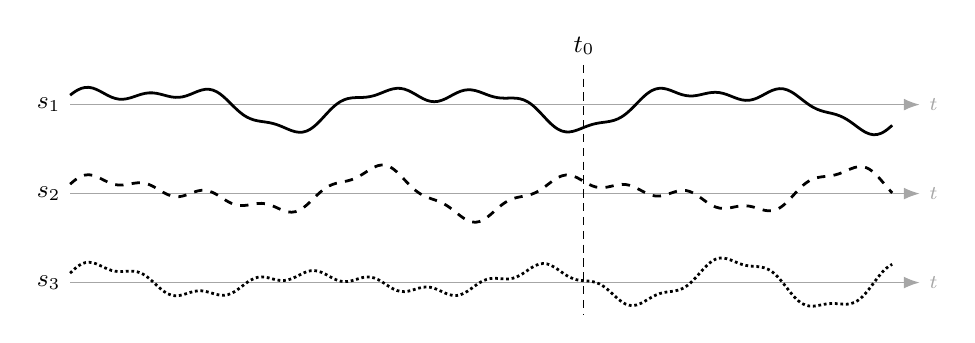
\begin{tikzpicture}[x=.87cm,y=.92cm]
  \foreach \k/\style in {0/solid,1/dashed,2/densely dotted}{
    \begin{scope}[yshift=-1.13*\k cm]
      \draw[-{Latex[length=2mm]},gray!70] (0,0)--(12.4,0) node[right,font=\scriptsize] {$t$};
      \draw[black,\style,line width=1pt,samples=220,domain=0:12,smooth]
        plot (\x,{.23*sin((85+19*\k)*\x)+.13*cos((169-12*\k)*\x)+.06*sin((390+20*\k)*\x)});
      \node[left,font=\small] at (0,0) {$s_{\the\numexpr\k+1\relax}$};
    \end{scope}}
  \draw[black,densely dashed] (7.5,.55)--(7.5,-2.9);
  \node[above,font=\small] at (7.5,.55) {$t_0$};
\end{tikzpicture}
\caption{Each trace fixes an experimental outcome $s_i$ and varies time. The vertical dashed line fixes time $t_0$ and compares outcomes.}
\label{fig:realizations}\end{figure}}

\newcommand{\MarginalFigure}{%
\begin{figure}[htbp]\centering
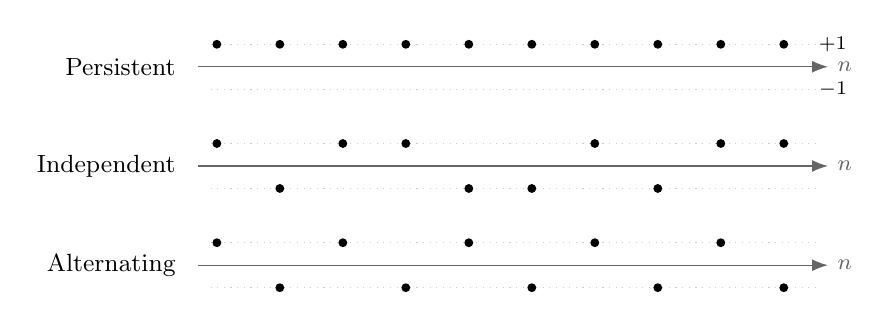
\begin{tikzpicture}[x=.8cm,y=.84cm]
  \foreach \y/\label in {3/Persistent,1.5/Independent,0/Alternating}{
    \draw[-{Latex[length=2mm]},black!60] (.7,\y)--(10.7,\y) node[right,font=\footnotesize] {$n$};
    \node[left,font=\small] at (.5,\y) {\label};
    \draw[black!20,dotted] (.9,{\y+.34})--(10.5,{\y+.34}) (.9,{\y-.34})--(10.5,{\y-.34});}
  \foreach \n in {1,...,10} {\fill[black] (\n,3.34) circle (1.6pt);}
  \foreach \n/\v in {1/1,2/-1,3/1,4/1,5/-1,6/-1,7/1,8/-1,9/1,10/1}
    {\fill[black] (\n,{1.5+.34*\v}) circle (1.6pt);}
  \foreach \n/\v in {1/1,2/-1,3/1,4/-1,5/1,6/-1,7/1,8/-1,9/1,10/-1}
    {\fill[black] (\n,{.34*\v}) circle (1.6pt);}
  \node[right,font=\scriptsize] at (10.4,3.34) {$+1$};
  \node[right,font=\scriptsize] at (10.4,2.66) {$-1$};
\end{tikzpicture}
\caption{Illustrative realizations of three processes with the same $50$--$50$ distribution at every time. Their temporal correlations and responses to averaging differ.}
\label{fig:marginals}\end{figure}}

\newcommand{\WindowOverlapFigure}{%
\begin{figure}[!ht]\centering
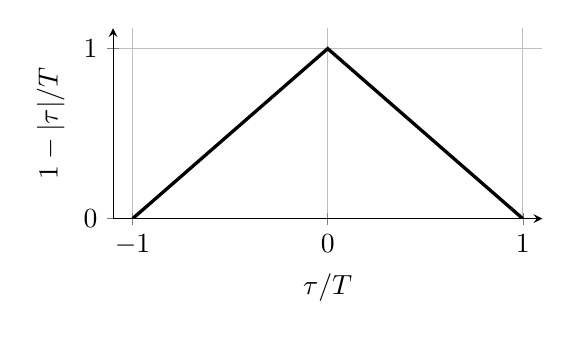
\begin{tikzpicture}
\begin{axis}[width=.58\linewidth,height=4cm,axis lines=left,
  xlabel={$\tau/T$},ylabel={$1-|\tau|/T$},
  xmin=-1.1,xmax=1.1,ymin=0,ymax=1.12,
  xtick={-1,0,1},ytick={0,1},grid=major]
  \addplot[black,very thick] coordinates {(-1,0) (0,1) (1,0)};
\end{axis}\end{tikzpicture}
\caption{The fraction of a length-$T$ observation interval shared with a copy shifted by $|\tau|$. Large lags have fewer pairs of observed samples.}
\label{fig:overlap}\end{figure}}

\newcommand{\LorentzianFigure}{%
\begin{figure}[htbp]\centering
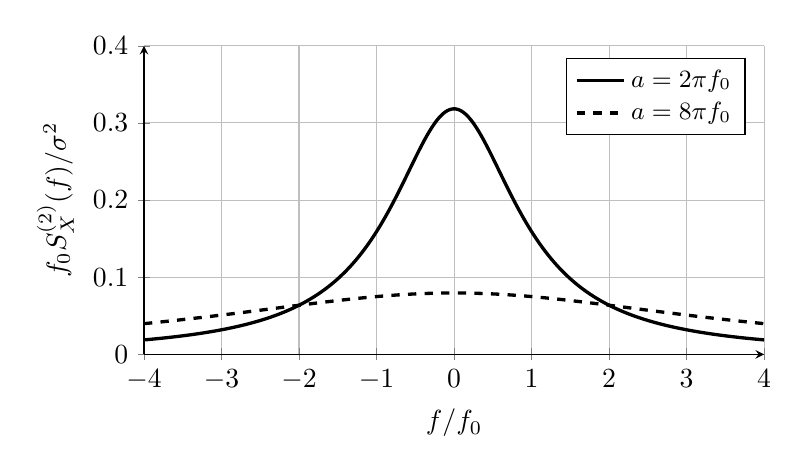
\begin{tikzpicture}
\begin{axis}[width=.78\linewidth,height=5.5cm,axis lines=left,
  xlabel={$f/f_0$},ylabel={$f_0S_X^{(2)}(f)/\sigma^2$},
  xmin=-4,xmax=4,ymin=0,ymax=.4,grid=major,
  legend style={at={(.97,.96)},anchor=north east,font=\small},samples=240]
  \addplot[black,very thick,domain=-4:4] {1/(pi*(1+x^2))};
  \addlegendentry{$a=2\pi f_0$}
  \addplot[black,very thick,dashed,domain=-4:4] {4/(pi*(16+x^2))};
  \addlegendentry{$a=8\pi f_0$}
\end{axis}
\end{tikzpicture}
\caption{Exponential correlations with the same variance $\sigma^2$, plotted using an arbitrary reference frequency $f_0>0$. Faster decorrelation ($a$ four times larger) spreads the same spectral area over a wider range of frequencies.}
\label{fig:lorentzian}\end{figure}}

\newcommand{\MatchedResistorFigure}{%
\begin{figure}[htbp]\centering
\begin{tikzpicture}[x=1cm,y=1cm,>=Latex]
  \draw (0,0)--(5.9,0);
  \draw (0,0)--(0,1.1);
  \draw (0,1.55) circle (.45);\node at (0,1.55) {$v_n$};
  \draw (0,2)--(0,2.45)--(1.82,2.45);
  \draw[decorate,decoration={zigzag,segment length=4pt,amplitude=1.7pt}]
    (1.82,2.45)--(2.38,2.45);
  \node[above] at (2.1,2.6) {$R$};
  \draw (2.38,2.45)--(5.9,2.45)--(5.9,1.55);
  \draw[decorate,decoration={zigzag,segment length=4pt,amplitude=1.7pt}]
    (5.9,1.55)--(5.9,.99);
  \draw (5.9,.99)--(5.9,0);
  \node[right] at (5.9,1.2) {$R_L=R$};
  \draw[<->,teal] (4.7,.12)--(4.7,2.32);
  \node[left,text=teal] at (4.7,1.22) {$v_L$};
\end{tikzpicture}
\caption{Matched load: half the source voltage and one quarter of its voltage-noise PSD.}
\label{fig:match}\end{figure}}

\newcommand{\NoiseBandwidthFigure}{%
\begin{figure}[htbp]\centering
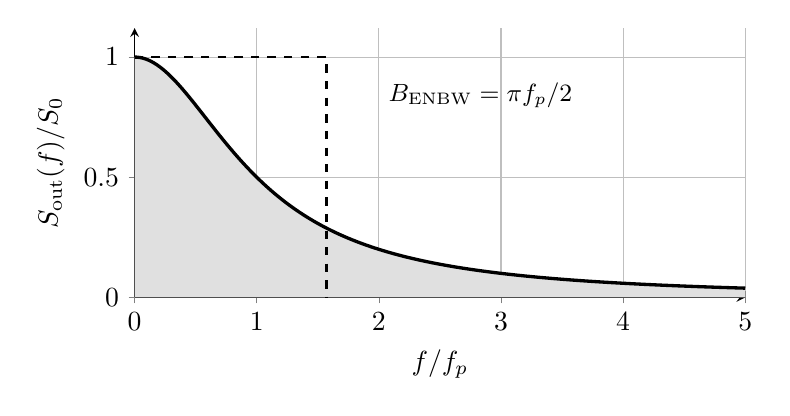
\begin{tikzpicture}
\begin{axis}[width=.77\linewidth,height=5cm,axis lines=left,
  xlabel={$f/f_p$},ylabel={$S_{\mathrm{out}}(f)/S_0$},
  xmin=0,xmax=5,ymin=0,ymax=1.12,grid=major,samples=220]
  \addplot[draw=none,fill=black!12,domain=0:5] {1/(1+x^2)} \closedcycle;
  \addplot[black,very thick,domain=0:5] {1/(1+x^2)};
  \addplot[black,dashed,thick] coordinates {(0,1) (1.5708,1) (1.5708,0)};
  \node[anchor=west,font=\small] at (axis cs:2.0,.84) {$B_{\enbw}=\pi f_p/2$};
\end{axis}\end{tikzpicture}
\caption{For unity DC gain, the one-pole PSD and the rectangle of height $S_0$ and width $B_{\enbw}=\pi f_p/2$ have equal total area. The response continues beyond the plotted range.}
\label{fig:enbw}\end{figure}}

\newcommand{\MultiPoleFigure}{%
\begin{figure}[htbp]\centering
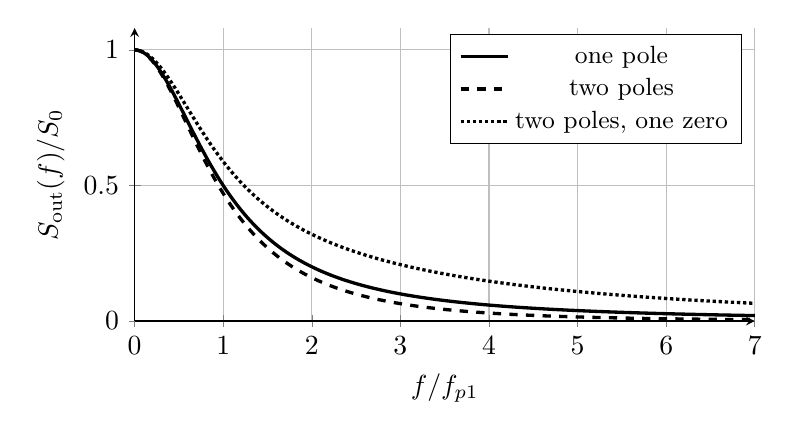
\begin{tikzpicture}
\begin{axis}[width=.78\linewidth,height=5.3cm,axis lines=left,
  xlabel={$f/f_{p1}$},ylabel={$S_{\mathrm{out}}(f)/S_0$},
  xmin=0,xmax=7,ymin=0,ymax=1.08,grid=major,samples=220,
  legend style={at={(.98,.98)},anchor=north east,font=\small}]
  \addplot[black,very thick,domain=0:7] {1/(1+x^2)};
  \addlegendentry{one pole}
  \addplot[black,very thick,dashed,domain=0:7] {1/((1+x^2)*(1+(x/4)^2))};
  \addlegendentry{two poles}
  \addplot[black,very thick,densely dotted,domain=0:7] {(1+(x/2)^2)/((1+x^2)*(1+(x/4)^2))};
  \addlegendentry{two poles, one zero}
\end{axis}\end{tikzpicture}
\caption{Normalized white-noise output spectra for $f_{p2}=4f_{p1}$ and $f_z=2f_{p1}$. A second pole reduces high-frequency area; a zero between the poles increases it.}
\label{fig:multipole}\end{figure}}


\newcommand{\FIRFigure}{%
\begin{figure}[htbp]\centering
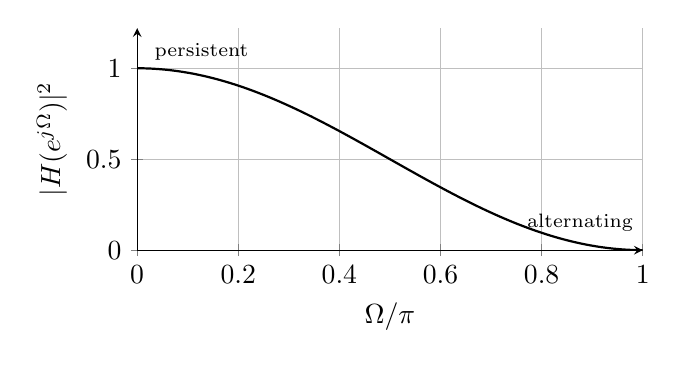
\begin{tikzpicture}
\begin{axis}[width=.66\linewidth,height=4.4cm,xmin=0,xmax=1,ymin=0,ymax=1.22,
 axis lines=left,xlabel={$\Omega/\pi$},ylabel={$|H(e^{j\Omega})|^2$},grid=major]
\addplot[black,thick,domain=0:1,samples=100]{cos(90*x)^2};
\node[font=\scriptsize,anchor=north west] at (axis cs:.015,1.19){persistent};
\node[font=\scriptsize,anchor=south east] at (axis cs:1,.05){alternating};
\end{axis}\end{tikzpicture}
\caption{The two-tap averager has unity gain at DC and a zero at Nyquist. For independent samples, the output variance is half the input variance.}
\end{figure}}

\newcommand{\EnsembleFigure}{%
\begin{figure}[htbp]\centering
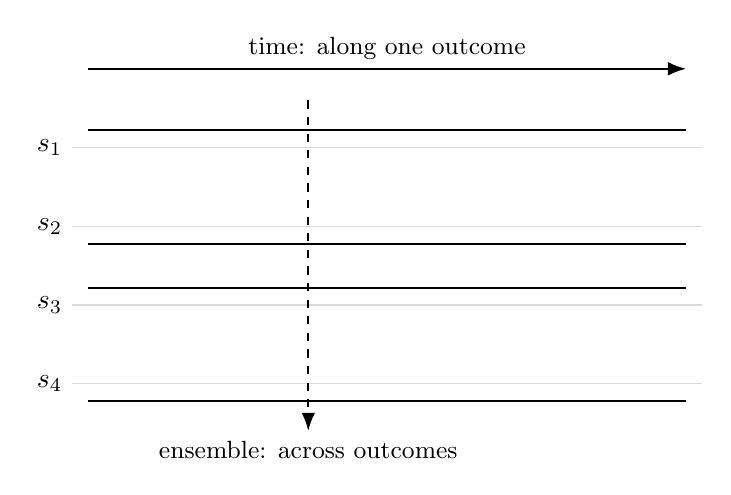
\begin{tikzpicture}[x=1cm,y=1cm,>=Latex]
\foreach \y/\lab/\v in {0/s_4/-1,1/s_3/1,2/s_2/-1,3/s_1/1}{
\draw[gray!30] (0,\y)--(8,\y);
\node[left] at (0,\y){$\lab$};
\draw[thick] (.2,{\y+.22*\v})--(7.8,{\y+.22*\v});}
\draw[->,dashed,thick] (3,3.6)--(3,-.6);
\node[below,font=\small] at (3,-.6){ensemble: across outcomes};
\draw[->,thick] (.2,4)--(7.8,4);
\node[above,font=\small] at (4,4){time: along one outcome};
\end{tikzpicture}
\caption{The persistent coin process: every row is a constant $+1$ or $-1$ relative to its own baseline. Averaging many independent records estimates the zero ensemble mean; extending one record leaves its time average unchanged.}
\end{figure}}

\newcommand{\OverlapIntervalsFigure}{%
\begin{figure}[htbp]\centering
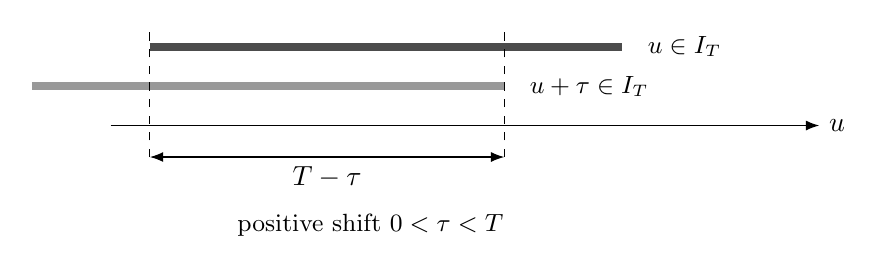
\begin{tikzpicture}[x=1cm,y=1cm,>=Latex]
\draw[->](-.5,0)--(8.5,0) node[right]{$u$};
\draw[line width=3pt,black!70] (0,1)--(6,1);
\draw[line width=3pt,black!40] (-1.5,.5)--(4.5,.5);
\draw[<->] (0,-.4)--(4.5,-.4) node[midway,below]{$T-\tau$};
\draw[dashed] (0,-.4)--(0,1.2) (4.5,-.4)--(4.5,1.2);
\node[right,font=\small] at (6.2,1){$u\in I_T$};
\node[right,font=\small] at (4.7,.5){$u+\tau\in I_T$};
\node[below,font=\small] at (2.8,-1){positive shift $0<\tau<T$};
\end{tikzpicture}
\caption{Only the shared interval contains pairs with both $t_2=u$ and $t_1=u+\tau$ inside the recorded window. For a negative shift the same argument gives $T-|\tau|$.}
\end{figure}}


\newcommand{\SpectrumConventionFigure}{%
\begin{figure}[htbp]\centering
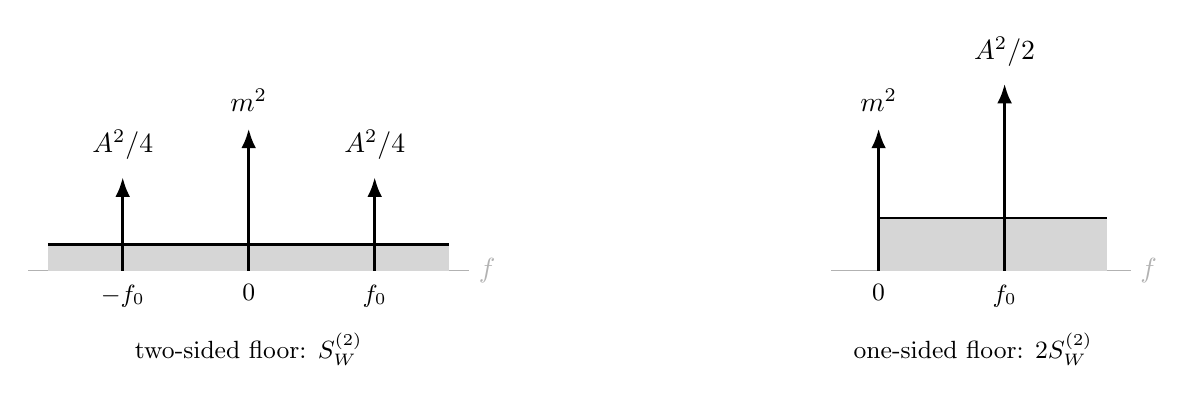
\begin{tikzpicture}[x=1cm,y=.95cm]
\begin{scope}
\draw[gray!60](-2.8,0)--(2.8,0) node[right]{$f$};
\fill[black!16](-2.55,0)rectangle(2.55,.35);
\draw[black,thick](-2.55,.35)--(2.55,.35);
\draw[-{Latex[length=2.5mm]},black,very thick](-1.6,0)--(-1.6,1.25);
\draw[-{Latex[length=2.5mm]},black,very thick](1.6,0)--(1.6,1.25);
\draw[-{Latex[length=2.5mm]},black,very thick](0,0)--(0,1.9);
\node[above] at (-1.6,1.35){$A^2/4$};\node[above] at (1.6,1.35){$A^2/4$};
\node[above] at (0,2){$m^2$};
\foreach \x/\lab in {-1.6/-f_0,0/0,1.6/f_0}{\node[below,font=\small]at(\x,-.06){$\lab$};}
\node[font=\small]at(0,-1.05){two-sided floor: $S_W^{(2)}$};
\end{scope}
\begin{scope}[xshift=8cm]
\draw[gray!60](-.6,0)--(3.2,0) node[right]{$f$};
\fill[black!16](0,0)rectangle(2.9,.7);
\draw[black,thick](0,.7)--(2.9,.7);
\draw[-{Latex[length=2.5mm]},black,very thick](0,0)--(0,1.9);
\draw[-{Latex[length=2.5mm]},black,very thick](1.6,0)--(1.6,2.5);
\node[above]at(0,2){$m^2$};\node[above]at(1.6,2.6){$A^2/2$};
\node[below,font=\small]at(0,-.06){$0$};\node[below,font=\small]at(1.6,-.06){$f_0$};
\node[font=\small]at(1.2,-1.05){one-sided floor: $2S_W^{(2)}$};
\end{scope}
\end{tikzpicture}
\caption{Two-sided and one-sided spectra. Shading denotes continuous noise density; arrows denote spectral masses, labeled by their values.}
\label{fig:spectral-masses}\end{figure}}

\newcommand{\RCFigure}{%
\begin{figure}[htbp]\centering
\begin{tikzpicture}[>=Latex]
\draw (0,0)--(5,0); \draw (0,0)--(0,.8);
\draw (0,1.2) circle (.4); \node at (0,1.2){$e_R$};
\draw (0,1.6)--(0,2)--(1.5,2);
\draw[decorate,decoration={zigzag,segment length=4pt,amplitude=1.7pt}](1.5,2)--(2.06,2);
\node[above] at (1.78,2.1){$R$};
\draw (2.06,2)--(5,2);\fill (4,2) circle(1.5pt);
\draw (4,2)--(4,1.18) (3.65,1.18)--(4.35,1.18) (3.65,1.02)--(4.35,1.02) (4,1.02)--(4,0);
\node[right] at (4.4,1.1){$C$}; \node[right] at (5,2){$v_C$};
\end{tikzpicture}
\caption{Resistor noise drives an ideal capacitor through the RC low-pass response.}
\end{figure}}

\newcommand{\NoiseCirclesFigure}{%
\begin{figure}[htbp]\centering
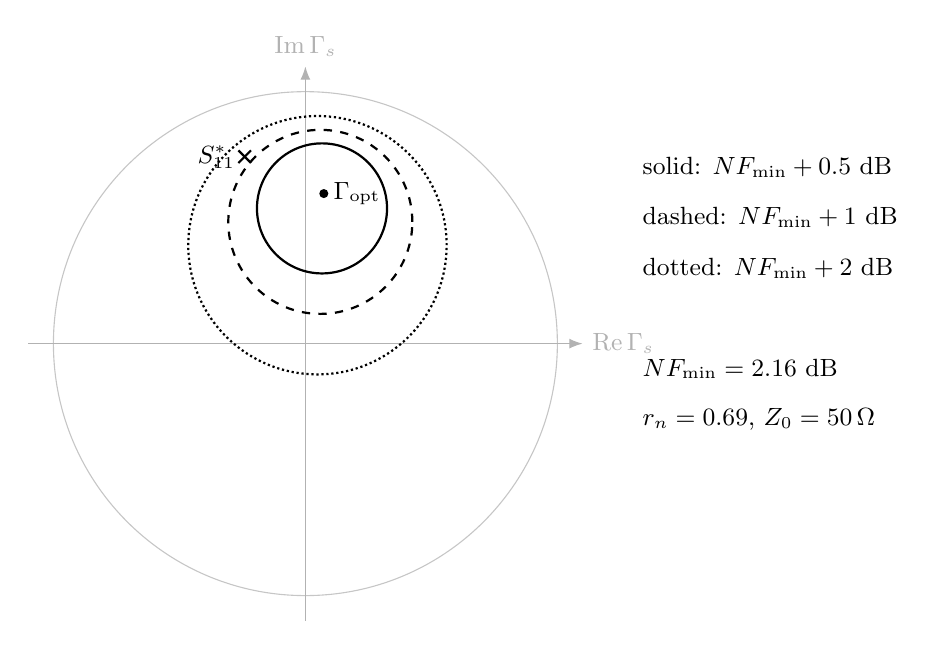
\begin{tikzpicture}[x=3.2cm,y=3.2cm,>=Latex]
\draw[gray!45] (0,0) circle(1);\draw[->,gray!60](-1.1,0)--(1.1,0) node[right,font=\small]{$\operatorname{Re}\Gamma_s$};
\draw[->,gray!60](0,-1.1)--(0,1.1) node[above,font=\small]{$\operatorname{Im}\Gamma_s$};
\foreach \d/\style in {.5/solid,1/dashed,2/densely dotted}{
\pgfmathsetmacro{\Nn}{(pow(10,(2.16+\d)/10)-pow(10,2.16/10))*(1+.36+1.2*cos(83))/(4*.69)}
\pgfmathsetmacro{\cx}{.60*cos(83)/(1+\Nn)}
\pgfmathsetmacro{\cy}{.60*sin(83)/(1+\Nn)}
\pgfmathsetmacro{\rr}{sqrt(\Nn*(1+\Nn-.36))/(1+\Nn)}
\draw[thick,\style] (\cx,\cy) circle(\rr);}
\fill ({.6*cos(83)},{.6*sin(83)}) circle(.018) node[right,font=\small]{$\Gamma_{\mathrm{opt}}$};
\draw[thick] ({.78*cos(108)-.025},{.78*sin(108)-.025})--({.78*cos(108)+.025},{.78*sin(108)+.025});
\draw[thick] ({.78*cos(108)-.025},{.78*sin(108)+.025})--({.78*cos(108)+.025},{.78*sin(108)-.025});
\node[left,font=\small] at ({.78*cos(108)},{.78*sin(108)}){$S_{11}^*$};
\node[font=\small,anchor=west] at (1.3,.7){solid: $NF_{\min}+0.5$ dB};
\node[font=\small,anchor=west] at (1.3,.5){dashed: $NF_{\min}+1$ dB};
\node[font=\small,anchor=west] at (1.3,.3){dotted: $NF_{\min}+2$ dB};
\node[font=\small,anchor=west] at (1.3,-.1){$NF_{\min}=2.16$ dB};
\node[font=\small,anchor=west] at (1.3,-.3){$r_n=0.69$, $Z_0=50\,\Omega$};
\end{tikzpicture}
\caption{Constant noise-figure circles in the reflection-coefficient plane for the illustrative noise parameters. The unit circle bounds passive source impedances. The noise optimum (dot) differs from the unilateral gain optimum (cross).}
\label{fig:noise-circles}\end{figure}}

\newcommand{\CorrelationPairFigure}{%
\begin{figure}[htbp]\centering
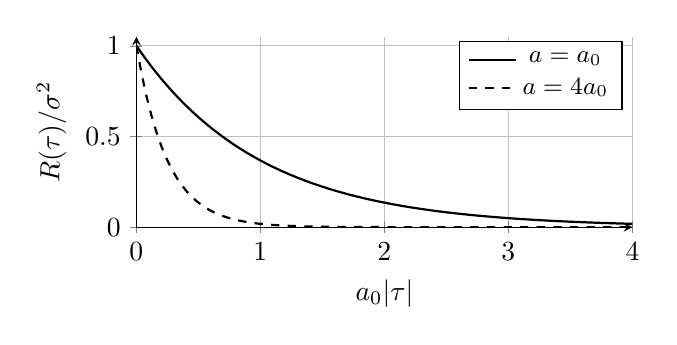
\begin{tikzpicture}
\begin{axis}[width=.65\linewidth,height=4cm,axis lines=left,xlabel={$a_0|\tau|$},ylabel={$R(\tau)/\sigma^2$},xmin=0,xmax=4,ymin=0,ymax=1.05,grid=major,
legend style={font=\small},samples=100]
\addplot[black,thick,domain=0:4]{exp(-x)};\addlegendentry{$a=a_0$}
\addplot[black,thick,dashed,domain=0:4]{exp(-4*x)};\addlegendentry{$a=4a_0$}
\end{axis}\end{tikzpicture}
\caption{The time-domain partner of Figure~\ref{fig:lorentzian}, with $a_0=2\pi f_0$. Shorter correlation time gives a wider PSD while leaving zero-lag variance fixed.}
\end{figure}}


\newcommand{\WKRegionsFigure}{%
\begin{figure}[!ht]\centering
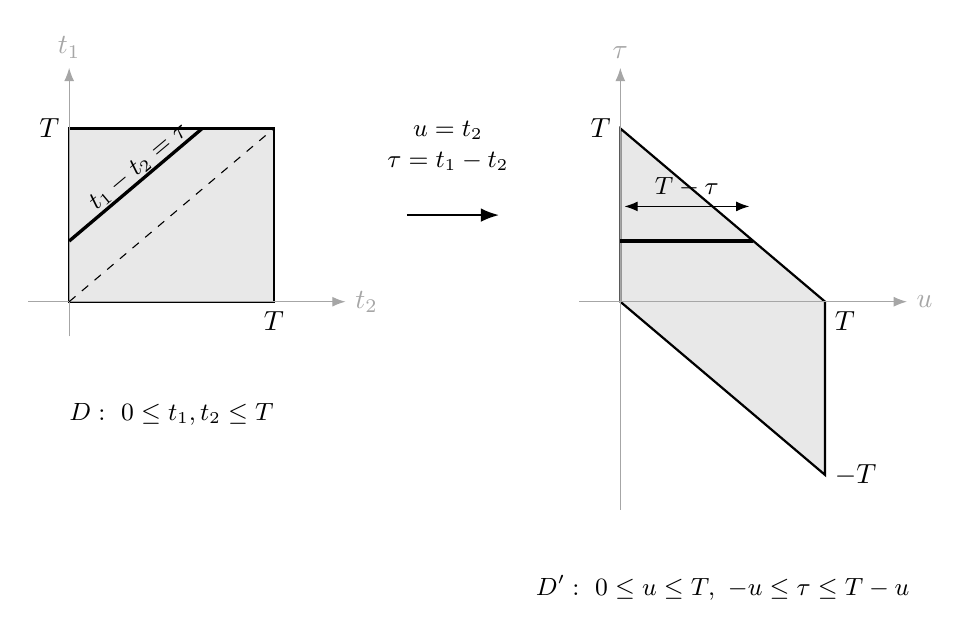
\begin{tikzpicture}[x=2.6cm,y=2.2cm,>=Latex]
\begin{scope}
\fill[black!9](0,0)rectangle(1,1);
\draw[thick](0,0)rectangle(1,1);
\draw[->,gray!70](-.2,0)--(1.35,0)node[right]{$t_2$};
\draw[->,gray!70](0,-.2)--(0,1.35)node[above]{$t_1$};
\draw[dashed](0,0)--(1,1);
\draw[very thick](0,.35)--(.65,1);
\node[font=\small,rotate=40]at(.34,.78){$t_1-t_2=\tau$};
\node[below]at(1,0){$T$};\node[left]at(0,1){$T$};
\node[font=\small]at(.5,-.65){$D:\ 0\leq t_1,t_2\leq T$};
\end{scope}
\draw[->,thick](1.65,.5)--(2.1,.5);
\node[font=\small,align=center]at(1.85,.9){$u=t_2$\\$\tau=t_1-t_2$};
\begin{scope}[xshift=7cm]
\fill[black!9](0,0)--(0,1)--(1,0)--(1,-1)--cycle;
\draw[thick](0,0)--(0,1)--(1,0)--(1,-1)--cycle;
\draw[->,gray!70](-.2,0)--(1.4,0)node[right]{$u$};
\draw[->,gray!70](0,-1.2)--(0,1.35)node[above]{$\tau$};
\draw[very thick](0,.35)--(.65,.35);
\draw[<->] (.02,.55)--(.63,.55)node[midway,above,font=\small]{$T-\tau$};
\node[left]at(0,1){$T$};\node[below right]at(1,0){$T$};
\node[right]at(1,-1){$-T$};
\node[font=\small]at(.5,-1.65){$D':\ 0\leq u\leq T,\ -u\leq\tau\leq T-u$};
\end{scope}
\end{tikzpicture}
\caption{The square of recorded time pairs and its image under the linear change of variables. The bold segment on the left becomes a fixed-$\tau$ horizontal slice on the right. For $\tau>0$ its length is $T-\tau$; for $\tau<0$ it is $T+\tau$.}
\label{fig:wk-regions}\end{figure}}

\newcommand{\InputReferralFigure}{%
\begin{figure}[htbp]\centering
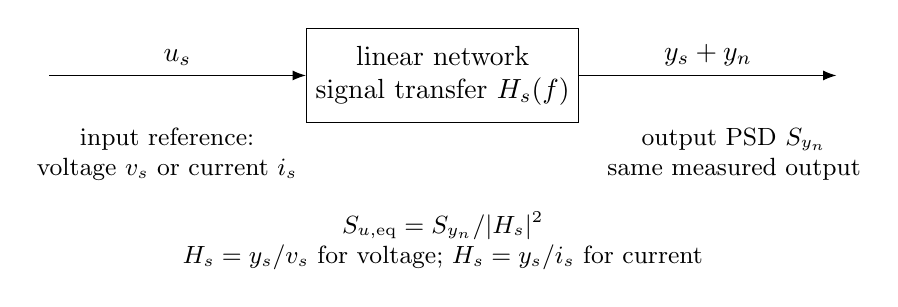
\begin{tikzpicture}[>=Latex]
\node[draw,minimum width=3.2cm,minimum height=1.2cm,align=center](net)at(5,0){linear network\\signal transfer $H_s(f)$};
\draw[->](0,0)--(net.west)node[midway,above]{$u_s$};
\draw[->](net.east)--(10,0)node[midway,above]{$y_s+y_n$};
\node[font=\small,align=center]at(1.5,-1){input reference:\\voltage $v_s$ or current $i_s$};
\node[font=\small,align=center]at(8.7,-1){output PSD $S_{y_n}$\\same measured output};
\node[font=\small,align=center]at(5,-2.1){$S_{u,\mathrm{eq}}=S_{y_n}/|H_s|^2$\\$H_s=y_s/v_s$ for voltage; $H_s=y_s/i_s$ for current};
\end{tikzpicture}
\caption{Input-referred noise reproduces the output PSD through the specified voltage or current signal transfer.}
\label{fig:input-referral}\end{figure}}

\newcommand{\TwoPortFigure}{%
\begin{figure}[!ht]\centering
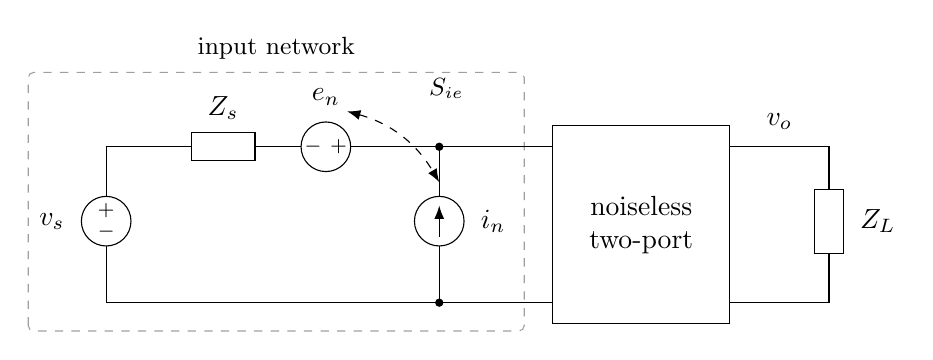
\begin{tikzpicture}[x=.9cm,y=.9cm,>=Latex]
\draw[dashed,gray!75,rounded corners=2pt](-1.1,-.4)rectangle(5.9,3.25);
\node[font=\small,above]at(2.4,3.3){input network};
\draw (0,0)--(6.3,0);\draw (0,0)--(0,.8);
\draw (0,1.15)circle(.35);\node[left]at(-.45,1.15){$v_s$};
\node[font=\scriptsize]at(0,1.3){$+$};\node[font=\scriptsize]at(0,1){$-$};
\draw (0,1.5)--(0,2.2)--(1.2,2.2);
\draw (1.2,2)rectangle(2.1,2.4);\node[above]at(1.65,2.45){$Z_s$};
\draw (2.1,2.2)--(2.75,2.2);
\draw (3.1,2.2)circle(.35);\node[above]at(3.1,2.65){$e_n$};
\node[font=\scriptsize]at(2.92,2.2){$-$};\node[font=\scriptsize]at(3.28,2.2){$+$};
\draw (3.45,2.2)--(6.3,2.2);
\draw (4.7,0)--(4.7,.8);\draw (4.7,1.15)circle(.35);
\draw[->](4.7,.93)--(4.7,1.37);\draw (4.7,1.5)--(4.7,2.2);
\node[right]at(5.15,1.15){$i_n$};
\fill(4.7,2.2)circle(1.5pt);\fill(4.7,0)circle(1.5pt);
\draw[dashed,<->](3.4,2.7)to[bend left=22](4.7,1.7);
\node[font=\small,above]at(4.8,2.75){$S_{ie}$};
\draw (6.3,-.3)rectangle(8.8,2.5);
\node[align=center]at(7.55,1.1){noiseless\\two-port};
\draw (8.8,2.2)--(10.2,2.2)--(10.2,1.6);
\draw (10,.7)rectangle(10.4,1.6);\draw (10.2,.7)--(10.2,0)--(8.8,0);
\node[right]at(10.5,1.15){$Z_L$};\node[above]at(9.5,2.3){$v_o$};

\end{tikzpicture}
\caption{Equivalent input voltage and current noise; the dashed network is converted to Norton form below.}
\label{fig:two-port}\end{figure}}

\newcommand{\NortonNoiseFigure}{%
\begin{figure}[!ht]\centering
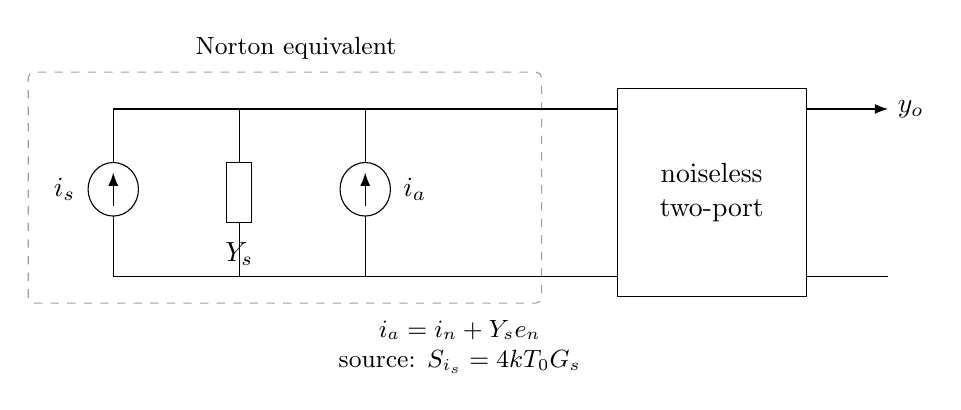
\begin{tikzpicture}[x=.8cm,y=.85cm,>=Latex]
\draw[dashed,gray!75,rounded corners=2pt](-1.35,-.4)rectangle(6.8,3.05);
\node[font=\small,above]at(2.9,3.1){Norton equivalent};
\draw (0,0)--(8,0);\draw (0,2.5)--(8,2.5);
\foreach \x/\lab in {0/i_s,4/i_a}{
\draw (\x,0)--(\x,.9);\draw (\x,1.3)circle(.4);\draw[->](\x,1.05)--(\x,1.55);\draw (\x,1.7)--(\x,2.5);
}\node[left]at(-.45,1.3){$i_s$};\node[right]at(4.45,1.3){$i_a$};
\draw (2,0)--(2,.8);\draw (1.8,.8)rectangle(2.2,1.7);\draw (2,1.7)--(2,2.5);
\node[below]at(2,.65){$Y_s$};
\draw (8,-.3)rectangle(11,2.8);\node[align=center]at(9.5,1.25){noiseless\\two-port};
\draw[->](11,2.5)--(12.3,2.5)node[right]{$y_o$};\draw (11,0)--(12.3,0);
\node[font=\small,align=center]at(5.5,-1.05){$i_a=i_n+Y_se_n$\\source: $S_{i_s}=4kT_0G_s$};
\end{tikzpicture}
\caption{Input Norton equivalent: source noise $i_s$ and added noise $i_a$ drive the same node.}
\label{fig:norton-noise}\end{figure}}

\newcommand{\ProjectionFigure}{%
\begin{figure}[htbp]\centering
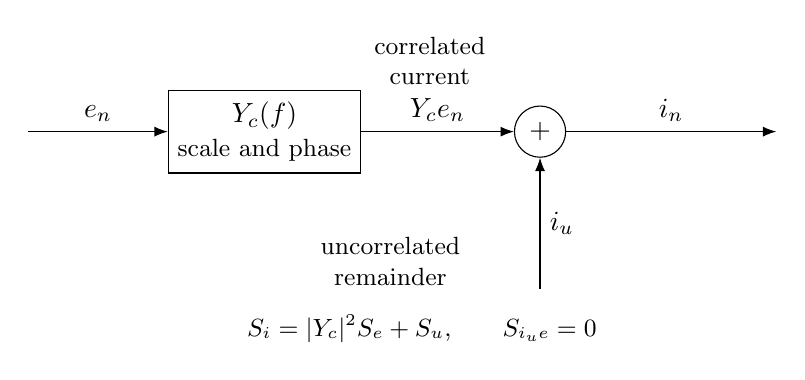
\begin{tikzpicture}[>=Latex]
\node[draw,minimum width=2.1cm,minimum height=1.05cm,align=center](yc)at(3,1){$Y_c(f)$\\\small scale and phase};
\node[draw,circle,minimum size=.65cm,inner sep=0pt](add)at(6.5,1){$+$};
\draw[->](0,1)--(yc.west)node[midway,above]{$e_n$};
\draw[->](yc.east)--(add.west)node[midway,above]{$Y_ce_n$};
\node[font=\small,align=center]at(5.1,1.9){correlated\\current};
\draw[->](6.5,-1)--(add.south)node[midway,right]{$i_u$};
\node[font=\small,align=center]at(4.6,-.65){uncorrelated\\remainder};
\draw[->](add.east)--(9.5,1)node[midway,above]{$i_n$};
\node[font=\small]at(5,-1.5){$S_i=|Y_c|^2S_e+S_u$,\qquad $S_{i_ue}=0$};
\end{tikzpicture}
\caption{The current noise is a voltage-correlated component plus an uncorrelated remainder.}
\label{fig:projection}\end{figure}}

\newcommand{\AdmittanceCancellationFigure}{%
\begin{figure}[htbp]\centering
\begin{tikzpicture}[x=2.5cm,y=1.5cm,>=Latex]
\draw[->,gray!70](-.4,0)--(2,0)node[right]{$G$ (mS)};
\draw[->,gray!70](0,-1.5)--(0,1.6)node[above]{$B$ (mS)};
\draw[->,thick](0,0)--(0,1)node[left]{$Y_c=j1$};
\draw[->,thick](0,0)--(1,-1)node[below right]{$Y_s=1-j1$};
\draw[->,very thick](0,0)--(1,0)node[midway,above]{$Y_s+Y_c=1$};
\draw[->,dashed](1,-1)--(1,0)node[midway,right,font=\small]{$+Y_c$};
\node[below left,font=\small]at(0,0){$0$};
\end{tikzpicture}
\caption{Source susceptance cancels the imaginary part of $Y_s+Y_c$ in the numerical example.}
\label{fig:admittance-cancellation}\end{figure}}

\newcommand{\FriisFigure}{%
\begin{figure}[htbp]\centering
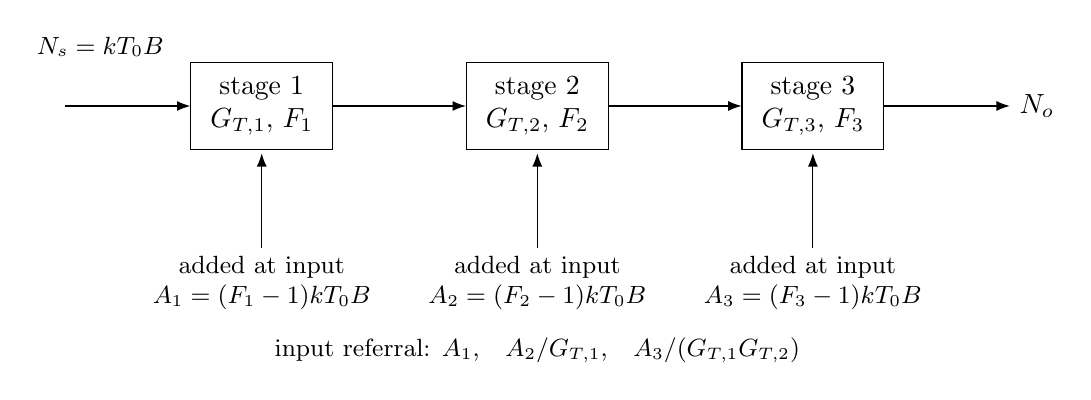
\begin{tikzpicture}[>=Latex]
\foreach \x/\j in {2.5/1,6/2,9.5/3}{
\node[draw,minimum width=1.8cm,minimum height=1.1cm,align=center](g\j)at(\x,0){stage $\j$\\$G_{T,\j}$, $F_\j$};
\draw[->](\x,-1.8)--(\x,-.6);
\node[font=\small,align=center]at(\x,-2.25){added at input\\$A_\j=(F_\j-1)kT_0B$};}
\draw[->](0,0)--(g1.west);\node[font=\small]at(.45,.75){$N_s=kT_0B$};
\draw[->](g1.east)--(g2.west);\draw[->](g2.east)--(g3.west);
\draw[->](g3.east)--(12,0)node[right]{$N_o$};
\node[font=\small]at(6,-3.1){input referral: $A_1$,\quad $A_2/G_{T,1}$,\quad $A_3/(G_{T,1}G_{T,2})$};
\end{tikzpicture}
\caption{Matched cascade with independent stage-added noise. Each $A_j$ is referred to its own stage input, before the gain.}
\label{fig:friis}\end{figure}}

\newcommand{\PhaseNoiseFigure}{%
\begin{figure}[htbp]\centering
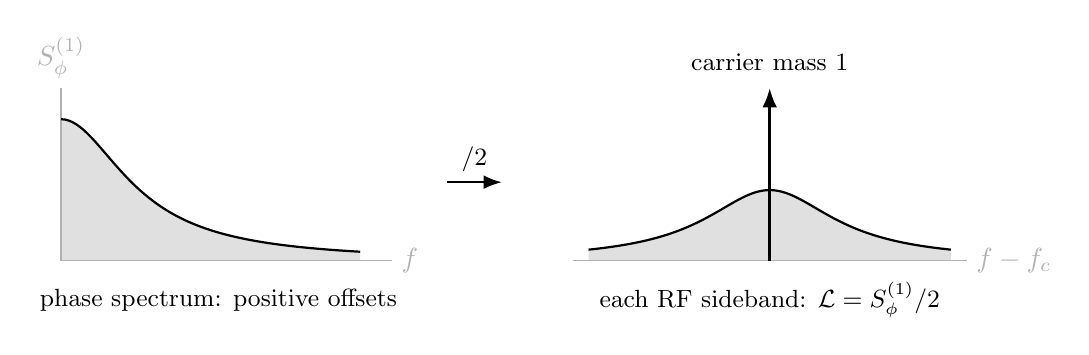
\begin{tikzpicture}[x=1cm,y=1cm,>=Latex]
\begin{scope}
\fill[black!12] (0,0) -- plot[domain=0:3.8,samples=80] (\x,{1.8/(1+\x*\x)}) -- (3.8,0) -- cycle;
\draw[gray!60](0,0)--(4.2,0)node[right]{$f$};
\draw[gray!60](0,0)--(0,2.2)node[above]{$S_\phi^{(1)}$};
\draw[thick,domain=0:3.8,samples=80]plot(\x,{1.8/(1+\x*\x)});
\node[font=\small]at(2,-.5){phase spectrum: positive offsets};
\end{scope}
\draw[->,thick](4.9,1)--(5.6,1)node[midway,above,font=\small]{$/2$};
\begin{scope}[xshift=9cm]
\fill[black!12] (-2.3,0) -- plot[domain=-2.3:2.3,samples=100] (\x,{.9/(1+\x*\x)}) -- (2.3,0) -- cycle;
\draw[gray!60](-2.5,0)--(2.5,0)node[right]{$f-f_c$};
\draw[thick,domain=-2.3:2.3,samples=100]plot(\x,{.9/(1+\x*\x)});
\draw[-{Latex[length=2.5mm]},very thick](0,0)--(0,2.2);
\node[above,font=\small]at(0,2.3){carrier mass $1$};
\node[font=\small]at(0,-.5){each RF sideband: $\mathcal L=S_\phi^{(1)}/2$};
\end{scope}
\end{tikzpicture}
\caption{Small phase fluctuations produce two RF noise sidebands. The right plot shows one-sided RF noise normalized to carrier power, with frequency measured relative to the positive carrier.}
\label{fig:phase-noise}\end{figure}}

\newcommand{\MeanErrorRegionsFigure}{%
\begin{figure}[htbp]\centering
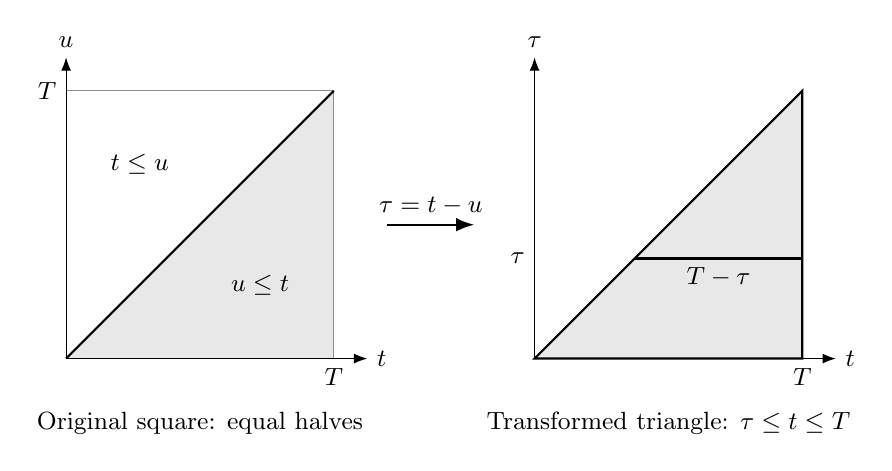
\begin{tikzpicture}[scale=.85,font=\small]
\begin{scope}
\fill[black!9] (0,0)--(4,0)--(4,4)--cycle;
\draw[black!45] (0,0) rectangle (4,4);
\draw[thick] (0,0)--(4,4);
\draw[-{Latex}] (0,0)--(4.5,0) node[right] {$t$};
\draw[-{Latex}] (0,0)--(0,4.5) node[above] {$u$};
\node[below] at (4,0) {$T$};\node[left] at (0,4) {$T$};
\node at (2.9,1.1) {$u\leq t$};\node at (1.1,2.9) {$t\leq u$};
\node[below] at (2,-.65) {Original square: equal halves};
\end{scope}
\draw[-{Latex},thick] (4.8,2)--(6.1,2) node[midway,above] {$\tau=t-u$};
\begin{scope}[xshift=7cm]
\fill[black!9] (0,0)--(4,0)--(4,4)--cycle;
\draw[thick] (0,0)--(4,0)--(4,4)--cycle;
\draw[-{Latex}] (0,0)--(4.5,0) node[right] {$t$};
\draw[-{Latex}] (0,0)--(0,4.5) node[above] {$\tau$};
\draw[very thick] (1.5,1.5)--(4,1.5);
\node[below] at (2.75,1.5) {$T-\tau$};
\node[left] at (0,1.5) {$\tau$};\node[below] at (4,0) {$T$};
\node[below] at (2,-.65) {Transformed triangle: $\tau\leq t\leq T$};
\end{scope}
\end{tikzpicture}
\caption{Even covariance gives equal contributions from the two halves of the original square. Transforming the lower half to $(t,\tau)$ gives a triangle. At fixed lag $\tau$, the horizontal interval has length $T-\tau$.}
\label{fig:mean-regions}\end{figure}}

\newcommand{\CorrelationAveragingFigure}{%
\begin{figure}[htbp]\centering
\begin{tikzpicture}
\begin{axis}[width=.47\linewidth,height=4cm,xmin=0,xmax=12,ymin=-3.5,ymax=3.5,
title={Short correlation: $\tau_c=0.4t_0$},title style={font=\small},
xlabel={$t/t_0$},ylabel={$X(t)/\sigma$},tick label style={font=\scriptsize},label style={font=\small}]
\addplot[black,thin] table[x=t,y=fast]{figures/correlation_averaging_data.dat};
\addplot[black!45,dashed,domain=0:12]{0};
\end{axis}
\begin{scope}[xshift=7.9cm]
\begin{axis}[width=.47\linewidth,height=4cm,xmin=0,xmax=12,ymin=-3.5,ymax=3.5,
title={Long correlation: $\tau_c=4t_0$},title style={font=\small},
xlabel={$t/t_0$},tick label style={font=\scriptsize},label style={font=\small}]
\addplot[black,thin] table[x=t,y=slow]{figures/correlation_averaging_data.dat};
\addplot[black!45,dashed,domain=0:12]{0};
\end{axis}\end{scope}
\begin{scope}[yshift=-4.7cm]
\begin{axis}[width=.47\linewidth,height=4.2cm,xmin=0,xmax=12,ymin=0,ymax=1.1,
title={Model autocovariance},title style={font=\small},xlabel={$\tau/t_0$},
ylabel={$C_X(\tau)/\sigma^2$},tick label style={font=\scriptsize},label style={font=\small},
legend style={font=\scriptsize,at={(.5,-.53)},anchor=north,legend columns=3,draw=none,fill=none}]
\addplot[black,thick,domain=0:12,samples=120]{exp(-x/.4)};\addlegendentry{Short}
\addplot[black,thick,dashed,domain=0:12,samples=120]{exp(-x/4)};\addlegendentry{Long}
\addplot[black,densely dotted,thick,domain=0:12]{1};\addlegendentry{Persistent}
\end{axis}\end{scope}
\begin{scope}[xshift=7.9cm,yshift=-4.7cm]
\begin{axis}[width=.47\linewidth,height=4.2cm,xmin=0,xmax=12,ymin=0,ymax=1.1,
title={Mean-estimation error},title style={font=\small},xlabel={$T/t_0$},
ylabel={$\operatorname{MSE}(T)/\sigma^2$},tick label style={font=\scriptsize},label style={font=\small}]
\addplot[black,thick,domain=.005:12,samples=150]{2*.4/x*(1-.4/x*(1-exp(-x/.4)))};
\addplot[black,thick,dashed,domain=.005:12,samples=150]{2*4/x*(1-4/x*(1-exp(-x/4)))};
\addplot[black,densely dotted,thick,domain=0:12]{1};
\end{axis}\end{scope}
\end{tikzpicture}
\caption{Stationary Gaussian records with equal variance and different correlation times. The lower panels compare their model covariances and exact mean-estimation MSEs with those of a persistent random offset. Time is normalized by $t_0$.}
\label{fig:correlation-averaging}\end{figure}}

\newcommand{\PeriodogramScatterFigure}{%
\begin{figure}[!htbp]\centering
\begin{tikzpicture}
\begin{axis}[width=.88\linewidth,height=3.0cm,xmin=0,xmax=.125,ymin=0,ymax=10,
title={One record: $N=256$},title style={font=\small},
ylabel={$I/S_0$},xticklabels=\empty,tick label style={font=\scriptsize},label style={font=\small}]
\addplot[black,thin] table[x=f,y=psd]{figures/periodogram_short.dat};
\addplot[black!55,dashed,domain=0:.125]{1};
\end{axis}
\begin{scope}[yshift=-3.25cm]
\begin{axis}[width=.88\linewidth,height=3.0cm,xmin=0,xmax=.125,ymin=0,ymax=10,
title={One record: $N=4096$},title style={font=\small},
ylabel={$I/S_0$},xticklabels=\empty,tick label style={font=\scriptsize},label style={font=\small}]
\addplot[black,thin] table[x=f,y=psd]{figures/periodogram_long.dat};
\addplot[black!55,dashed,domain=0:.125]{1};
\end{axis}\end{scope}
\begin{scope}[yshift=-6.5cm]
\begin{axis}[width=.88\linewidth,height=3.0cm,xmin=0,xmax=.125,ymin=0,ymax=10,
title={Average of 32 independent records: $N=4096$ each},title style={font=\small},
xlabel={$f\Delta t$},ylabel={$I/S_0$},xtick={0,.025,.05,.075,.1,.125},xticklabels={0,0.025,0.05,0.075,0.10,0.125},scaled x ticks=false,tick label style={font=\scriptsize},label style={font=\small}]
\addplot[black,thin] table[x=f,y=psd]{figures/periodogram_averaged.dat};
\addplot[black!55,dashed,domain=0:.125]{1};
\end{axis}\end{scope}
\end{tikzpicture}
\caption{FFT periodograms of independent, unit-variance Gaussian samples on common axes. The dashed line is the true normalized PSD. A longer record narrows bin spacing; averaging 32 independent records reduces scatter. The flat source spectrum has no window bias at these FFT bins.}
\label{fig:periodogram-scatter}\end{figure}}

\newcommand{\MixerImageNoiseFigure}{%
\begin{figure}[!htbp]\centering
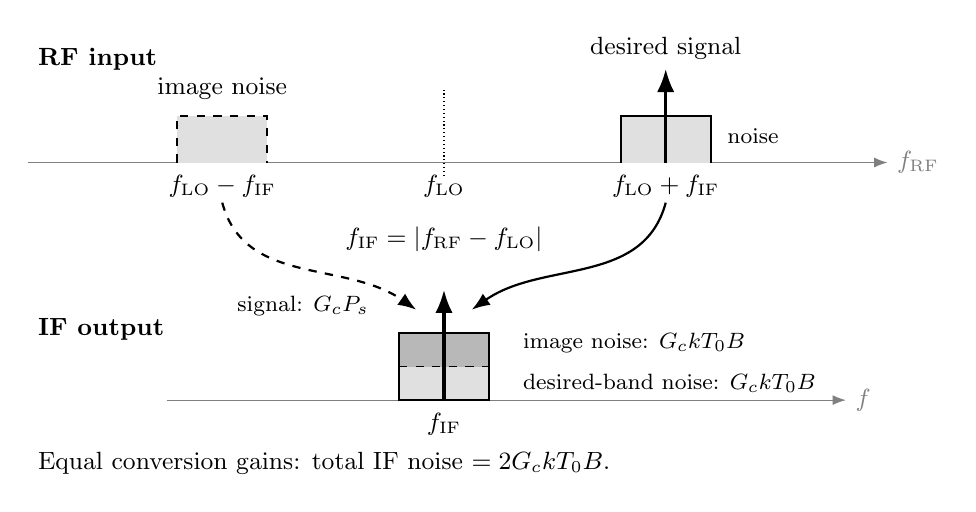
\begin{tikzpicture}[x=.88cm,y=.85cm,>=Latex,font=\small]
  \node[anchor=west,font=\bfseries\small] at (0,4.8) {RF input};
  \draw[->,gray] (0,3.25)--(12.4,3.25) node[right] {$f_{\mathrm{RF}}$};
  \fill[black!12] (2.15,3.25) rectangle (3.45,3.95);
  \draw[dashed,thick] (2.15,3.25)--(2.15,3.95)--(3.45,3.95)--(3.45,3.25);
  \fill[black!12] (8.55,3.25) rectangle (9.85,3.95);
  \draw[thick] (8.55,3.25)--(8.55,3.95)--(9.85,3.95)--(9.85,3.25);
  \draw[->,very thick] (9.2,3.25)--(9.2,4.65);
  \node[above] at (2.8,4.05) {image noise};
  \node[above] at (9.2,4.65) {desired signal};
  \node[anchor=west,font=\footnotesize] at (9.95,3.65) {noise};
  \draw[densely dotted] (6,3.05)--(6,4.35);
  \node[below] at (6,3.2) {$f_{\mathrm{LO}}$};
  \node[below] at (2.8,3.2) {$f_{\mathrm{LO}}-f_{\mathrm{IF}}$};
  \node[below] at (9.2,3.2) {$f_{\mathrm{LO}}+f_{\mathrm{IF}}$};
  \draw[->,thick,dashed] (2.8,2.65) to[out=-75,in=145] (5.6,1.05);
  \draw[->,thick] (9.2,2.65) to[out=-105,in=35] (6.4,1.05);
  \node[fill=white,inner sep=2pt] at (6,2.1) {$f_{\mathrm{IF}}=|f_{\mathrm{RF}}-f_{\mathrm{LO}}|$};
  \node[anchor=west,font=\bfseries\small] at (0,.75) {IF output};
  \draw[->,gray] (2,-.3)--(11.8,-.3) node[right] {$f$};
  \fill[black!12] (5.35,-.3) rectangle (6.65,.2);
  \fill[black!28] (5.35,.2) rectangle (6.65,.7);
  \draw[thick] (5.35,-.3) rectangle (6.65,.7);
  \draw[dashed] (5.35,.2)--(6.65,.2);
  \draw[->,very thick] (6,-.3)--(6,1.35);
  \node[below] at (6,-.35) {$f_{\mathrm{IF}}$};
  \node[anchor=west,font=\footnotesize] at (7,.55) {image noise: $G_c kT_0B$};
  \node[anchor=west,font=\footnotesize] at (7,-.05) {desired-band noise: $G_c kT_0B$};
  \node[anchor=east,font=\footnotesize] at (5.05,1.1) {signal: $G_cP_s$};
  \node[anchor=west] at (0,-1.25) {Equal conversion gains: total IF noise $=2G_ckT_0B$.};
\end{tikzpicture}
\caption{Noise from the desired and image bands adds at IF; shading shows the two contributions.}
\label{fig:mixer-image-noise}
\end{figure}}

\newcommand{\CorrelationSpectrumFigure}{%
\begin{figure}[htbp]\centering
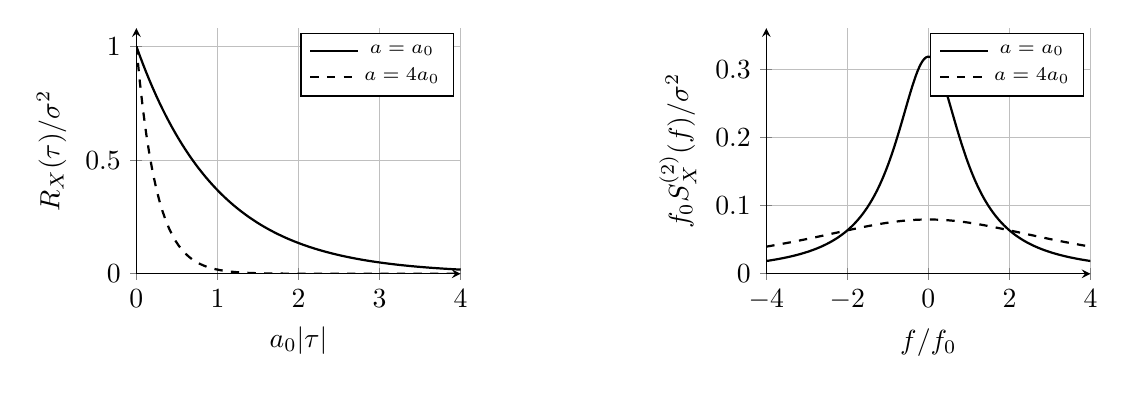
\begin{tikzpicture}
\begin{axis}[width=.47\linewidth,height=4.7cm,axis lines=left,
xlabel={$a_0|\tau|$},ylabel={$R_X(\tau)/\sigma^2$},
xmin=0,xmax=4,ymin=0,ymax=1.08,grid=major,
legend style={font=\scriptsize,at={(.98,.98)},anchor=north east},samples=100]
\addplot[black,thick,domain=0:4]{exp(-x)};\addlegendentry{$a=a_0$}
\addplot[black,thick,dashed,domain=0:4]{exp(-4*x)};\addlegendentry{$a=4a_0$}
\end{axis}
\begin{scope}[xshift=8.0cm]
\begin{axis}[width=.47\linewidth,height=4.7cm,axis lines=left,
xlabel={$f/f_0$},ylabel={$f_0S_X^{(2)}(f)/\sigma^2$},
xmin=-4,xmax=4,ymin=0,ymax=.36,grid=major,samples=200,
legend style={font=\scriptsize,at={(.98,.98)},anchor=north east}]
\addplot[black,thick,domain=-4:4]{1/(pi*(1+x^2))};\addlegendentry{$a=a_0$}
\addplot[black,thick,dashed,domain=-4:4]{4/(pi*(16+x^2))};\addlegendentry{$a=4a_0$}
\end{axis}\end{scope}
\end{tikzpicture}
\caption{Correlation and its Lorentzian spectrum, with $a_0=2\pi f_0$. Faster decorrelation broadens the spectrum while preserving the variance.}
\label{fig:lorentzian}\end{figure}}


\begin{document}
\hypersetup{pageanchor=false}
\begin{titlepage}
\thispagestyle{empty}
\vspace*{32mm}
{\sffamily\large ANALOG AND RF INTEGRATED CIRCUITS}\par
\vspace{9mm}\rule{\linewidth}{1.2pt}\par
\vspace{19mm}
{\sffamily\bfseries\fontsize{34}{41}\selectfont The Nature of Noise}\par
\vspace{8mm}
{\sffamily\fontsize{18}{26}\selectfont From random motion to spectral density,\par
 thermal equilibrium, and circuit analysis}\par
\vspace{18mm}
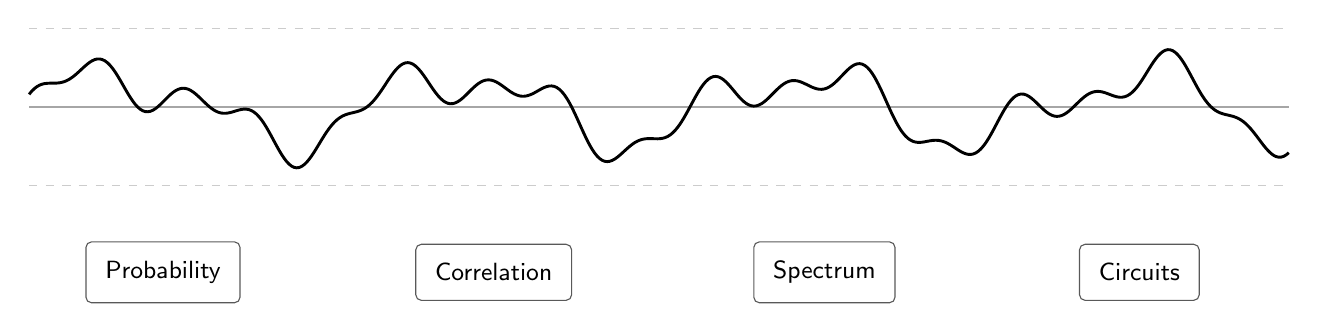
\begin{tikzpicture}[x=1cm,y=1cm]
  \draw[black!35] (0,0)--(16,0);
  \draw[black!20,dashed] (0,1)--(16,1) (0,-1)--(16,-1);
  \draw[black,line width=1.05pt,samples=500,domain=0:16,smooth]
    plot (\x,{.40*sin(83*\x)+.24*sin(179*\x)+.16*cos(373*\x)});
  \foreach \x/\label in {1.7/Probability,5.9/Correlation,10.1/Spectrum,14.1/Circuits}
    \node[draw=black!65,rounded corners=2pt,fill=white,
      text=black,font=\sffamily\small,inner sep=7pt] at (\x,-2.1) {\label};
\end{tikzpicture}
\vfill
{\sffamily\large Mingyang Zhang}\par
\vspace{3mm}{\sffamily\small October 2026}\par
\vspace{5mm}
{\sffamily\small For readers of analog electronics, integrated circuits, and RF systems}\par
\vspace{13mm}\rule{\linewidth}{.5pt}
\end{titlepage}
\thispagestyle{empty}
\vspace*{16mm}

{\sffamily\bfseries\large The Nature of Noise}\par
\vspace{2mm}
{\sffamily From Random Motion to Spectral Density,\par
Thermal Equilibrium, and Circuit Analysis}\par
\vspace{8mm}

Copyright \textcopyright\ 2026 Mingyang Zhang.

\vspace{5mm}
\begin{tabular}{@{}ll@{}}
\textbf{Author:} & Mingyang Zhang\\[2pt]
\textbf{Version:} & 1.0\\[2pt]
\textbf{First Public Release:} & October 18, 2026
\end{tabular}

\vspace{7mm}
This work is licensed under the\newline
\textbf{Creative Commons Attribution--\allowbreak NonCommercial--\allowbreak NoDerivatives 4.0 International License (CC BY-NC-ND 4.0)}.

You are free to copy and redistribute the unmodified work in any medium or format for noncommercial purposes, provided that appropriate credit is given to the author, a link to the license is included, and any other applicable license conditions are satisfied.

Adapted versions, including modified or translated editions, may not be shared without separate permission from the copyright holder, except as permitted by applicable law.

\textbf{License:} \url{https://creativecommons.org/licenses/by-nc-nd/4.0/}

\vspace{6mm}
{\sffamily\bfseries Citation}\par
\vspace{2mm}
Zhang, M. (2026). \emph{The Nature of Noise: From Random Motion to Spectral Density, Thermal Equilibrium, and Circuit Analysis}. Version 1.0.

\clearpage
\setcounter{page}{1}

\hypersetup{pageanchor=true}

\section*{Preface}
\addcontentsline{toc}{section}{Preface}
Record the same noise twice, and you will never get the same waveform. Yet its statistics can be strikingly reproducible: a fluctuating voltage may have a well-defined spectrum and a precise dependence on temperature. This raises some questions. How can a voltage with zero mean still deliver energy? Why do processes with identical voltage distributions respond so differently to averaging? And when can a single measured record reveal the statistics of an entire ensemble?

Correlation is the thread that ties random waveforms to their spectra. It determines which fluctuations survive averaging, and how a circuit reshapes their mean-square contribution. It also exposes a distinction at the heart of measurement: ensemble statistics describe a process, whereas statistics computed from one finite record are only estimates. Stationarity, ergodicity, and estimation error decide what a measured trace can, and cannot, tell us. They also explain why simply recording for longer does not guarantee a smoother or more accurate spectrum.

Thermal equilibrium gives these statistics a physical scale. The energy stored in a capacitor fixes the variance of its equilibrium voltage. The resistance connected to it sets the pace of relaxation and supplies the fluctuations that balance dissipation. From this picture follow $kT/C$ noise, resistor noise, and the available noise power $kTB$. Linear network analysis then carries noise from its physical sources to a measurable output, keeping track of the correlations that may reinforce or partially cancel one another.

The circuit viewpoint leads naturally to input-referred noise, noise factor, and the role of source impedance in RF design. Noise matching and power matching solve different optimization problems, and the noise of a cascade depends on where loss and gain are placed. Phase noise brings the story back to the time domain: fluctuations in a carrier's phase appear as spectral sidebands and timing jitter, and accumulated phase diffusion broadens the carrier line. Throughout, the aim stays the same: to trace a path from a physical source of randomness to the fluctuations that a measurement actually records.

\clearpage
\begingroup\small\setlength{\parskip}{0pt}\tableofcontents\endgroup
\clearpage

\section{Probability and random processes}
\subsection{Random variables, processes, and realizations}
For a sinusoid $x(t)=A\cos(2\pi f_0t+\phi)$, fixing $A$, $f_0$, and $\phi$ determines the voltage at every time. Repeating a thermal-noise measurement under unchanged macroscopic conditions gives a different trace each time. We therefore describe a family of possible waveforms together with their probabilities, rather than one predetermined waveform.

\paragraph{Outcomes, events, and probability.}
An \emph{outcome} $s$ is one complete possible result of the experiment. In a noise model, it specifies enough information to determine an entire voltage record, not just the voltage at one time. The \emph{sample space} $\Omega$ is the set of all possible outcomes.

An \emph{event} $A$ is a collection of outcomes to which the model assigns a probability $P(A)$. For example, ``the voltage at $t_0$ is positive'' selects every outcome whose record meets that condition. Formally, events are measurable subsets of $\Omega$; not every subset must be an event in a general model. In a finite model, we can take every subset as an event. The probability of the whole sample space is one, and probabilities of disjoint events add. Appendix~\ref{app:probability} states the general framework.

\paragraph{Random variables and random processes.}
A real \emph{random variable} is a function $Z:\Omega\to\mathbb R$: it assigns a number $Z(s)$ to each outcome. Its value becomes definite once the outcome is fixed. Its probabilities come from the outcomes, rather than from a separate assignment:
\[
P\{Z\leq z\}=P\bigl(\{s\in\Omega:Z(s)\leq z\}\bigr).
\]
The function must be measurable, meaning that each such set is an event. An outcome and the numerical value of a random variable are different objects; several outcomes can give the same value.

A real \emph{random process} is a family of random variables indexed by time, defined on the same probability space. We write
\begin{equation}
X(t,s),\qquad t\in\mathbb R,\quad s\in\Omega.
\label{eq:process}
\end{equation}
Its two arguments keep separate the time of observation and the outcome being observed:
\begin{itemize}
\item Fixing $s=s_i$ gives a \emph{realization} $x_i(t)=X(t,s_i)$: one waveform as time varies.
\item Fixing $t=t_0$ gives the random variable $X(t_0,\cdot)$: one voltage value for each possible outcome. Its probability distribution compares records at that same time.
\end{itemize}
The \emph{ensemble} is the family of possible realizations with the probability weighting inherited from the model. It is not a finite collection of measured traces; repeated experiments sample this ensemble. Different outcomes may produce the same realization.

\RealizationFigure

For example, let two independent fair coin tosses set voltages at $t_0$ and $t_1$: heads means $+1$ mV and tails means $-1$ mV. The complete outcomes are
\[
\Omega=\{HH,HT,TH,TT\},\qquad P(\{s\})=1/4.
\]
The event $A=\{s:X(t_0,s)>0\}=\{HH,HT\}$ contains two outcomes, so $P(A)=1/4+1/4=1/2$.
\begin{center}
\begin{tabular}{cccc}\toprule
Outcome $s$ & $P(\{s\})$ & $X(t_0,s)$ & $X(t_1,s)$\\\midrule
$HH$ & $1/4$ & $+1$ & $+1$\\
$HT$ & $1/4$ & $+1$ & $-1$\\
$TH$ & $1/4$ & $-1$ & $+1$\\
$TT$ & $1/4$ & $-1$ & $-1$\\\bottomrule
\end{tabular}\par\vspace{2mm}
{\small Voltages are in millivolts. A column fixes time; a row fixes an outcome.}
\end{center}
A column fixes time and lists the random variable's values across outcomes. A row fixes an outcome and gives two samples from its realization. Throughout the text, $\E$ denotes an average over outcomes, weighted by their probabilities.

\subsection{Ensemble mean, variance, and root-mean-square value}
An expectation is a probability-weighted average. If a random variable $Z$ takes values $z_i$ with probabilities $p_i$, then
\[
\E[Z]=\sum_i p_i z_i.
\]
If its values have a probability density $p_Z(z)$, the sum becomes
\[
\E[Z]=\int_{-\infty}^{\infty}z\,p_Z(z)\dd z.
\]
A density is probability per unit value: $p_Z(z)\dd z$ is the probability of a value in a small interval near $z$. Neither expression averages along time.

At each fixed time $t$, the process has a voltage distribution. Its ensemble mean is
\begin{equation}
\boxed{\mu_X(t)=\E[X(t)]=\int_{-\infty}^{\infty}x\,p_X(x;t)\dd x,}
\end{equation}
when a density exists; a discrete distribution uses the weighted sum instead. The semicolon in $p_X(x;t)$ emphasizes that $x$ is the integration variable and $t$ is held fixed.
The ensemble variance and RMS are
\begin{align}
\sigma_X^2(t)&=\E[(X(t)-\mu_X(t))^2],\\
X_{\rms}(t)&=\sqrt{\E[X(t)^2]}.
\end{align}
At fixed $t$, $\mu_X(t)$ is a number, so it can be taken outside the expectation. Expanding the square and using $\E[X(t)]=\mu_X(t)$ gives
\begin{align}
\sigma_X^2(t)&=\E[X(t)^2]-2\mu_X(t)\E[X(t)]+\mu_X(t)^2\notag\\
&=\E[X(t)^2]-\mu_X(t)^2.
\label{eq:variance}
\end{align}

The RMS includes the mean; standard deviation measures fluctuations about it. Neither is a time average by definition. In the coin example, at either fixed time $\E[X(t)]=0$ but $\E[X(t)^2]=(1\,\mathrm{mV})^2$. For a voltage across a resistor, the ensemble-average power is $\E[X(t)^2]/R>0$ despite the zero mean. Whether a measured time-average power equals this number is a separate question.

\begin{insight}[title={A Gaussian model describes the voltage distribution}]
A Gaussian random variable has the bell-shaped density
\[
p_X(x)=\frac{1}{\sqrt{2\pi}\sigma}
\exp\!\left[-\frac{(x-\mu)^2}{2\sigma^2}\right].
\]
Its mean $\mu$ locates the center and its standard deviation $\sigma$ sets the width. A histogram of repeated fixed-time measurements estimates this distribution. A histogram formed along one trace estimates it only under suitable averaging conditions.

A \emph{jointly Gaussian process} has Gaussian joint distributions for every finite collection of samples. This is stronger than requiring a Gaussian histogram at each time: it also specifies how samples depend on one another. Its mean and covariance determine all those joint distributions.
\end{insight}

\subsection{Temporal dependence and correlation}
\label{sec:temporal-dependence}
Consider samples $X_n(s)=X(nT_s,s)$ at sample interval $T_s$. At every fixed $n$, the following processes have probabilities $1/2$ for $+1$ and $-1$ V:
\begin{enumerate}
\item Persistent: select one fair random sign $A$ and set $X_n=A$ for all $n$.
\item Independent: select a fresh fair sign at each $n$.
\item Alternating: select one fair sign $A$ and set $X_n=(-1)^nA$.
\end{enumerate}
All three have ensemble mean zero and variance $1\,\mathrm{V}^2$ at every time. Now \emph{operate across two times within each realization}:
\[
Y_n(s)=\frac{X_n(s)+X_{n-1}(s)}{2}.
\]
This finite temporal filter is not an ensemble average. After filtering each waveform, we compute the ensemble output variance by fixing $n$ and averaging $Y_n(s)^2$ across outcomes:
\begin{align*}
\E[Y_n^2]
&=\frac14\E[(X_n+X_{n-1})^2]\\
&=\frac14\{\E[X_n^2]+\E[X_{n-1}^2]+2\E[X_nX_{n-1}]\}.
\end{align*}
For the persistent process $X_nX_{n-1}=A^2=1$; for independent signs its expectation factors as $\E[X_n]\E[X_{n-1}]=0$; for alternating signs $X_nX_{n-1}=-A^2=-1$. Since $\E[Y_n]=0$, the respective variances are $1$, $1/2$, and $0\,\mathrm{V}^2$. A fixed-time histogram cannot supply this cross-time information.
\MarginalFigure

The cross term distinguishes the three processes: adjacent fluctuations reinforce, cancel on average, or cancel exactly. The same product average applies to two voltages $U,V$ at different circuit nodes. Each pair must come from the same experimental outcome; pairing unrelated experiments would discard the dependence of interest.

\paragraph{Removing the mean: covariance.}
The sign examples have zero mean, so their voltages are already deviations about the mean. A practical voltage may also contain a DC bias. The product $\E[UV]$ then includes both the bias and the relation between the fluctuations. For example, let
\[
U=V_0+u,\qquad V=V_0+v,
\]
where $u$ and $v$ are independent zero-mean fluctuations. Expanding before taking the expectation gives
\[
\E[UV]=V_0^2+V_0\E[u]+V_0\E[v]+\E[uv]=V_0^2.
\]
The product average is positive even though the fluctuations are independent. To isolate the fluctuations, subtract the mean of each voltage before multiplying.

Define $\mu_U=\E[U]$, $\mu_V=\E[V]$, and the centered variables $U_c=U-\mu_U$, $V_c=V-\mu_V$. Their product average is the \emph{covariance}:
\begin{align}
\Cov(U,V)&=\E[U_cV_c]
=\E[(U-\mu_U)(V-\mu_V)]\\
&=\E[UV]-\mu_U\mu_V.
\end{align}
Covariance is the two-variable counterpart of variance: $\Cov(U,U)=\Var(U)$. Positive covariance means that deviations with the same sign dominate the product average; negative covariance means that deviations with opposite signs dominate. Neither statement requires every observed pair to have the corresponding signs.

For the sign examples, the adjacent-sample covariances are $+1$, $0$, and $-1\,\mathrm{V}^2$. For general means, center the two inputs first. Expanding $\E[(U_c+V_c)^2]/4$ gives

\[
\boxed{\Var\left(\frac{U+V}{2}\right)
=\frac14\{\Var(U)+\Var(V)+2\Cov(U,V)\}.}
\]
Positive covariance increases the output variance; negative covariance reduces it. Covariance describes exactly the additional information needed to calculate the noise of this temporal filter.

\paragraph{Removing the scale: the correlation coefficient.}
Covariance has units equal to the product of the units of $U$ and $V$. Doubling the amplitude of one voltage doubles their covariance, even if their pattern of dependence is unchanged. Dividing by the two standard deviations removes this scale dependence. For positive variances, the \emph{Pearson correlation coefficient} is
\[
\rho_{UV}=\frac{\Cov(U,V)}{\sigma_U\sigma_V},
\qquad \sigma_U=\sqrt{\Var(U)},\quad \sigma_V=\sqrt{\Var(V)}.
\]
It lies between $-1$ and $1$. To see the bound, normalize the centered variables: $u=U_c/\sigma_U$, $v=V_c/\sigma_V$. Then $\E[u^2]=\E[v^2]=1$ and $\E[uv]=\rho_{UV}$. Nonnegative squared deviations give
\[
0\leq\E[(u-v)^2]=2-2\rho_{UV},\qquad
0\leq\E[(u+v)^2]=2+2\rho_{UV},
\]
so $-1\leq\rho_{UV}\leq1$. The adjacent-sample coefficients of the persistent, independent, and alternating examples are respectively $+1$, $0$, and $-1$.

Zero covariance means that the centered product averages to zero. Independence guarantees this cancellation, but cancellation alone does not guarantee independence. For example, if $U$ takes $-1$, $0$, and $1$ with equal probability and $V=U^2$, then $\E[U]=\E[U^3]=0$ and
\[
\Cov(U,V)=\E[U^3]-\E[U]\E[U^2]=0.
\]
Nevertheless, $U$ determines $V$ exactly. For jointly Gaussian variables, zero covariance does imply independence.

\paragraph{Applying the definitions across time.}
For a random process, the two variables can be samples at fixed times:
$U(s)=X(t_1,s)$ and $V(s)=X(t_2,s)$. Their product average is called \emph{autocorrelation}; their covariance is called \emph{autocovariance}:
\begin{align}
R_X(t_1,t_2)&=\E[X(t_1)X(t_2)],\label{eq:autocorr}\\
C_X(t_1,t_2)&=\E[(X(t_1)-\mu_X(t_1))(X(t_2)-\mu_X(t_2))]\notag\\
&=R_X(t_1,t_2)-\mu_X(t_1)\mu_X(t_2).
\label{eq:covariance}
\end{align}
The prefix \emph{auto} indicates that both samples belong to the same process. The \emph{lag} $\tau=t_2-t_1$ is their time separation. These are functions of the chosen times; their expectation still averages over outcomes, not over time. Autocorrelation retains the mean contribution, whereas autocovariance isolates the fluctuations. In particular,
\[
R_X(t,t)=\E[X(t)^2],\qquad C_X(t,t)=\Var(X(t)).
\]
For a zero-mean process they coincide at every pair of times.

Unlike the Pearson coefficient $\rho$, the autocorrelation $R_X$ is unnormalized and retains units of voltage squared.

\begin{derivation}[title={Further connection: covariance and linear prediction}]
Suppose the centered voltage $U_c$ is used to predict $V_c$ by $bU_c$. Its mean-square prediction error is
\[
\E[(V_c-bU_c)^2]
=\Var(V)-2b\Cov(U,V)+b^2\Var(U).
\]
For $\Var(U)>0$, differentiation with respect to $b$ gives
\[
b_{\mathrm{opt}}=\frac{\Cov(U,V)}{\Var(U)},\qquad
\E[(V_c-b_{\mathrm{opt}}U_c)^2]
=\Var(V)-\frac{\Cov(U,V)^2}{\Var(U)}.
\]
The covariance determines how much a linear predictor can reduce the error. When it is zero, the best centered linear prediction is zero, even though nonlinear dependence may remain. The correlated voltage--current noise model in Chapter~5 uses the same idea at each frequency.
\end{derivation}

The two-tap average illustrates the time-domain role of correlation. After introducing spectra, we will revisit its frequency response in Section~\ref{sec:two-tap-spectrum}.

\subsection{Stationarity and ergodicity}
Two different questions arise in a noise measurement. Do the statistical properties change during the experiment? Can one sufficiently long record recover those properties? Stationarity addresses the first question; ergodicity addresses the second.
\label{sec:ergodicity}
\begin{concept}[title={Wide-sense stationarity}]
A real process with finite second moments is wide-sense stationary (WSS) if, for every time $t$ and lag $\tau$,
\[
\mu_X(t)=\mu,\qquad R_X(t,t+\tau)=R_X(\tau).
\]
Its autocovariance is $C_X(\tau)=R_X(\tau)-\mu^2$.
\end{concept}
WSS is a statement about \emph{ensemble} first and second moments. It does not make different times independent. Strict stationarity requires all joint distributions, rather than only the mean and autocorrelation, to be unchanged by a common time shift. Neither form of stationarity guarantees that a single record represents the ensemble.

For each fixed duration $T>0$, define the time-average \emph{estimator}
\begin{equation}
\overline X_T(s)=\frac1T\int_0^T X(t,s)\dd t.
\label{eq:time-estimator}
\end{equation}
Once a record is observed, $\overline x_T(s_i)$ is a number computed along that record. Before the outcome is observed, $\overline X_T$ is itself a random variable: different records give different estimates. Consequently $\E[\overline X_T]$ is an ensemble average of many possible time-average estimates. It must not be confused with the temporal integration inside each estimate.
\EnsembleFigure

\paragraph{Using a time average to estimate the ensemble mean.}
The ensemble mean $\mu$ is a property of the process, but a measurement usually supplies only one record. The time average $\overline X_T(s)$ is therefore used as an \emph{estimate} of $\mu$. For a particular record $s_i$, its estimation error is
\[
e_T(s_i)=\overline X_T(s_i)-\mu.
\]
Another possible record generally gives another error. Reliability cannot be judged from the signed average of those errors alone: positive and negative errors may cancel even when individual estimates are inaccurate. Squaring each error before averaging avoids that cancellation.

The \emph{mean-square error} (MSE) is the probability-weighted average of the squared estimation errors over all possible records:
\begin{equation}
\boxed{\operatorname{MSE}(T)=\E[|e_T|^2]
=\E[|\overline X_T-\mu|^2].}
\label{eq:mean-mse}
\end{equation}
The integral in $\overline X_T$ averages \emph{within one record}; the expectation in the MSE averages \emph{across possible records}. MSE measures error in the estimated mean, not the voltage's own variance. Its square root is the RMS estimation error, in volts.

Mean ergodicity asks whether a longer observation can make this error arbitrarily small.

\begin{concept}[title={Mean ergodicity}]
A WSS process is \emph{mean ergodic in mean square} if its time-average estimate of the ensemble mean has vanishing MSE:
\begin{equation}
\lim_{T\to\infty}\E[|\overline X_T-\mu|^2]=0.
\label{eq:mean-ergodic}
\end{equation}
This is a statement about estimation accuracy across the ensemble as record duration grows. It does not require any finite record to have exactly the ensemble mean, nor does stationarity alone guarantee it.
\end{concept}

\paragraph{Error probability.}
An EE measurement often specifies an allowed error $\epsilon$, such as $10\,\mu$V. The probability
$P\{|\overline X_T-\mu|\geq\epsilon\}$ is the fraction of possible records, weighted by their probabilities, whose mean estimates miss the target by at least that tolerance. For any fixed $\epsilon>0$,
\[
\boxed{P\{|\overline X_T-\mu|\geq\epsilon\}
\leq\frac{\operatorname{MSE}(T)}{\epsilon^2}.}
\]
The bound follows because every such record contributes at least $\epsilon^2$ to the squared error. Consequently, if MSE tends to zero, the probability of exceeding any fixed tolerance also tends to zero. For example, an RMS estimation error of $1\,\mu$V bounds the probability of an error of at least $10\,\mu$V by $(1/10)^2=0.01$.

This is a Chebyshev-type bound; Appendix~\ref{app:chebyshev} proves it from the nonnegative squared error. Mean-square convergence implies convergence in probability, but is distinct from convergence along almost every individual record. The latter, stronger pathwise question is discussed in Appendix~\ref{app:convergence}.

The persistent process $X(t,s)=A(s)$ is stationary, with ensemble mean zero and $C_X(\tau)=1\,\mathrm{V}^2$. Yet $\overline X_T(s)=A(s)$ for every $T$ and
$\E[|\overline X_T|^2]=1\,\mathrm{V}^2$. It is not mean ergodic: observing the same sign for longer cannot reveal the equally probable opposite sign in other outcomes.

\subsection{Estimating the ensemble mean from a time average}
\label{sec:mean-proof}
We now express the estimation error in terms of the covariance. First, the WSS time average is unbiased:
\begin{align*}
\E[\overline X_T]
&=\frac1T\int_0^T\E[X(t)]\dd t
=\frac1T\int_0^T\mu\dd t=\mu.
\end{align*}
The expectation and time integral can be exchanged because finite mean-square voltage implies $\E|X(t)|\leq\sqrt{\E[X(t)^2]}$, a finite constant on this interval (Appendix~\ref{app:integration}). Unbiasedness means that estimates average to $\mu$ across repeated records, not that each estimate equals $\mu$.

Set $Z(t)=X(t)-\mu$, so $\E[Z(t)]=0$. The estimation error is the time average of $Z$. Expanding its square gives
\begin{align*}
\operatorname{MSE}(T)
&=\E[|\overline X_T-\mu|^2]\\
&=\frac1{T^2}\E\left[\int_0^T\!\int_0^T Z(t)Z(u)\dd u\dd t\right]\\
&=\frac1{T^2}\int_0^T\!\int_0^T C_X(t-u)\dd u\dd t.
\end{align*}
The expectation and time integrals can be exchanged because
$\E|Z(t)Z(u)|\leq C_X(0)$, giving a finite absolute integral on the square.

\paragraph{Integrating over lag.}
For real WSS noise, shifting both sample times and reversing their order gives
\[
C_X(-\tau)=\E[Z(t)Z(t-\tau)]
=\E[Z(t+\tau)Z(t)]=C_X(\tau).
\]
The covariance is therefore even, so the two halves of the square $0\leq t,u\leq T$ contribute equally. On the lower half, set $\tau=t-u$:
\[
0\leq u\leq t\leq T
\quad\longrightarrow\quad
0\leq\tau\leq t\leq T.
\]
At fixed lag $\tau$, $t$ ranges from $\tau$ to $T$, as shown in Figure~\ref{fig:mean-regions}. Thus
\begin{align}
\operatorname{MSE}(T)
&=\frac2{T^2}\int_0^T\int_0^t C_X(t-u)\dd u\dd t\notag\\
&=\frac2{T^2}\int_0^T\int_0^t C_X(\tau)\dd\tau\dd t\notag\\
&=\frac2{T^2}\int_0^T\int_\tau^T C_X(\tau)\dd t\dd\tau\notag\\
&=\boxed{\frac2{T^2}\int_0^T(T-\tau)C_X(\tau)\dd\tau.}
\label{eq:mean-var}
\end{align}
The weight $T-\tau$ is the available interval for sample pairs separated by lag $\tau$.
\MeanErrorRegionsFigure

\paragraph{Why temporal correlation determines averaging accuracy.}
For noise with short correlation time, widely separated parts of a record contribute weakly related fluctuations. A longer record then averages over more such fluctuations, reducing the estimation error. If the noise remains strongly correlated throughout the observation, extending the record mostly repeats information already present. The relevant quantity is the autocovariance, not how jagged or smooth one waveform appears.

A useful sufficient condition is finite absolute covariance area:
\[
\int_0^\infty|C_X(\tau)|\dd\tau<\infty.
\]
In Eq.~\eqref{eq:mean-var}, replace $C_X$ by its absolute value and use $T-\tau\leq T$. Then
\[
0\leq\operatorname{MSE}(T)
\leq\frac2T\int_0^T|C_X(\tau)|\dd\tau
\leq\frac2T\int_0^\infty|C_X(\tau)|\dd\tau\longrightarrow0.
\]
The final area is fixed, so the bound decreases as $1/T$. This condition is sufficient, not necessary: positive and negative correlations can also cancel. The exact criterion is the limit of Eq.~\eqref{eq:mean-var}. Figure~\ref{fig:correlation-averaging} compares short correlation, long correlation, and a persistent random offset.

\CorrelationAveragingFigure

\paragraph{Exponential covariance: the role of correlation time.}
For $C_X(\tau)=\sigma^2e^{-a|\tau|}$, $a>0$, use integration by parts with $u=T-\tau$ and $\dd v=e^{-a\tau}\dd\tau$:
\begin{align*}
\int_0^T(T-\tau)e^{-a\tau}\dd\tau
&=\left[-\frac{T-\tau}{a}e^{-a\tau}\right]_0^T
-\frac1a\int_0^T e^{-a\tau}\dd\tau\\
&=\frac{T}{a}-\frac{1-e^{-aT}}{a^2}.
\end{align*}

Substitution into Eq.~\eqref{eq:mean-var} yields
\begin{equation}
\operatorname{MSE}(T)=\frac{2\sigma^2}{aT}
\left[1-\frac{1-e^{-aT}}{aT}\right].
\end{equation}
For $aT\ll1$, $e^{-aT}=1-aT+(aT)^2/2+O((aT)^3)$, so the MSE tends to $\sigma^2$: a short record contains strongly correlated samples. For $aT\gg1$ the MSE is approximately $2\sigma^2/(aT)$. Equating this to the variance $\sigma^2/N$ of $N$ independent observations defines a variance-equivalent sample count $N_{\mathrm{eff}}\simeq aT/2$. It is a comparison of estimation errors, not a claim that correlated samples become literally independent.

\begin{example}[title={How long must a record be to estimate the mean?}]
Suppose a zero-mean voltage has RMS fluctuation $\sigma=1$ mV and correlation time $1/a=1\,\mu$s. For a $1$-ms record, $aT=1000$, so
\[
\sqrt{\operatorname{MSE}(T)}
\simeq\sigma\sqrt{\frac{2}{aT}}
=44.7\,\mu\mathrm V.
\]
The mean of an individual trace need not be zero; its typical estimation error is about $45\,\mu$V. Making the record ten times longer reduces this RMS error by $\sqrt{10}$, rather than by ten. Sampling the same record more densely does not supply the same benefit, because nearby samples remain correlated.
\end{example}

For $X(t)=A+W(t)$, where $A$ is an independent random offset of variance $\sigma_A^2$ and $W$ has mean zero and integrable covariance,
$C_X(\tau)=\sigma_A^2+C_W(\tau)$. Equation~\eqref{eq:mean-var} then gives
$\operatorname{MSE}(T)=\sigma_A^2+\operatorname{MSE}_W(T)\to\sigma_A^2$.
A longer record cannot average away the outcome-specific offset. Subtracting each record's mean intentionally removes this information from a spectral estimate.

\subsection{Correlation ergodicity}
\label{sec:corr-ergodicity}
A PSD is determined by second-order statistics, so consistent estimation of the mean alone is insufficient. For fixed $\tau\geq0$, define
\[
\widehat R_T(\tau,s)=\frac1T\int_0^T X(t,s)X(t+\tau,s)\dd t.
\]
The estimator requires a record on $[0,T+\tau]$. The process is \emph{correlation ergodic in mean square at lag $\tau$} when
\begin{equation}
\E[|\widehat R_T(\tau)-R_X(\tau)|^2]\longrightarrow0.
\end{equation}
For covariance, the mean is subtracted before forming products. If the mean is estimated from the record, that estimation error must also be accounted for.

To estimate correlation at lag $\tau$, average products of samples separated by that lag. The product $X(t)X(t+\tau)$ fluctuates from one time pair to another, just as $X(t)$ itself fluctuates. Correlation averaging succeeds when these product fluctuations lose their dependence over sufficiently long time separations. Decay of the original voltage covariance alone is not enough: the error of a product average involves products of four voltage samples.

\paragraph{A sufficient condition.}
Treat the sample product as a new random process:
\[
Q_\tau(t)=X(t)X(t+\tau),\qquad
K_\tau(u)=\Cov(Q_\tau(t),Q_\tau(t+u)).
\]
Here $\tau$ separates the samples within a pair; $u$ separates two pairs. For a stationary process with finite fourth moment, $Q_\tau$ has stationary, finite-variance statistics. Its mean is $R_X(\tau)$, so estimating correlation is the mean-estimation problem applied to $Q_\tau$. Equation~\eqref{eq:mean-var} therefore gives
\[
\E|\widehat R_T(\tau)-R_X(\tau)|^2
\leq\frac2T\int_0^\infty|K_\tau(u)|\dd u.
\]
Thus finite absolute product-covariance area ensures correlation ergodicity at that lag. Gaussianity is not required. It is enough for $X$ to be WSS and $Q_\tau$ to have the stationary statistics used here; full stationarity is a convenient stronger assumption. Appendix~\ref{app:correlation-proof} develops the fourth-order and sampled-data details.

The test concerns the measured, bandwidth-limited output, including correlations among sources. Thermal noise, filtered shot noise, and random-telegraph noise can satisfy it under suitable models. Drift, random offsets, and persistent noise-intensity variations can prevent product-covariance decay. An ideal $1/f$ law extending to zero lacks finite variance; ideal white noise needs filtering before this finite-moment test applies.

\paragraph{The Gaussian RC model as an example.}
For a zero-mean stationary Gaussian process with exponential covariance
$C_X(\tau)=\sigma^2e^{-a|\tau|}$, both kinds of fluctuations decay. The correlation estimate satisfies
\[
\E[|\widehat R_T(\tau)-R_X(\tau)|^2]\leq\frac{2\sigma^4}{aT}.
\]
The error vanishes for every fixed lag. For Gaussian noise, voltage covariance determines product covariance; more generally, $\int_{\mathbb R}C_X(u)^2\dd u<\infty$ is sufficient. Appendix~\ref{app:correlation-proof} derives the bound, and Appendix~\ref{app:almost-sure} gives an optional almost-sure proof for sampled Gaussian RC noise.

To see why voltage-covariance decay alone is insufficient, let $X_n=B W_n$, where $W_n$ are independent fair signs and $B$ is independently selected once as $1$ or $2$ V with equal probability. Then $\E X_n=0$ and
$\Var(N^{-1}\sum X_n)=\E[B^2]/N\to0$.
But $N^{-1}\sum X_n^2=B^2$ for every record, whereas $R_X[0]=\E[B^2]=2.5\,\mathrm{V}^2$. The process is mean ergodic but not correlation ergodic: a single record retains a random noise intensity. Correlation ergodicity alone does not make the raw periodogram consistent (Section~\ref{sec:psd-measurement}).




\section{From correlation to spectral density}
\subsection{Fourier representation and finite observation}
For a finite pulse, the Fourier transform describes how its energy is distributed over frequency. Noise persists throughout an observation, so its accumulated energy increases with record duration. A noise PSD instead describes mean-square voltage per unit bandwidth. The normalization by record duration makes that distinction precise.
For a deterministic waveform, Fourier transformation separates temporal dependence into sinusoidal components. With $f$ in hertz and $j^2=-1$, our transform convention is
\begin{equation}
\widehat x(f)=\int_{\mathbb R}x(t)e^{-j2\pi ft}\dd t,\qquad
x(t)=\int_{\mathbb R}\widehat x(f)e^{j2\pi ft}\dd f.
\label{eq:fourier}
\end{equation}
The inverse formula applies when the waveform satisfies the usual Fourier inversion conditions; finite-energy signals also admit a mean-square interpretation. The factor $2\pi$ converts cycles per second to radians per second.

\begin{concept}[title={Parseval--Plancherel theorem}]
For a finite-energy waveform, $\int_{\mathbb R}|x(t)|^2\dd t<\infty$, its Fourier transform satisfies
\begin{equation}
\boxed{\int_{\mathbb R}|x(t)|^2\dd t
=\int_{\mathbb R}|\widehat x(f)|^2\dd f.}
\label{eq:parseval}
\end{equation}
There is no $2\pi$ factor with the hertz convention in Eq.~\eqref{eq:fourier}. The two integrals measure the same signal energy in different coordinates. For a voltage waveform, this signal-energy quantity has units V$^2\cdot$s; division by a resistance converts it to physical energy in joules.
\end{concept}
For a smooth finite-support waveform, substitute the inverse transform for the second factor:
\begin{align*}
\int x(t)^*x(t)\dd t
&=\int x(t)^*\left[\int\widehat x(f)e^{j2\pi ft}\dd f\right]\dd t\\
&=\int\widehat x(f)\left[\int x(t)^*e^{j2\pi ft}\dd t\right]\dd f\\
&=\int|\widehat x(f)|^2\dd f.
\end{align*}
The middle step exchanges the integration order; the bracket is $\widehat x(f)^*$. Approximation extends this argument to all finite-energy waveforms.

For WSS noise with finite mean square $R_X(0)=\E[X(t)^2]$, a duration-$T$ record has expected squared-voltage integral
\[
\E\left[\int_0^T X(t)^2\dd t\right]
=\int_0^T\E[X(t)^2]\dd t=T R_X(0).
\]
The expectation can pass through the integral because the squared voltage is nonnegative. When $R_X(0)>0$, the expected squared-voltage integral grows with $T$; an infinite noise record is not generally a finite-energy signal. However, its windowed transform is well defined:
\begin{equation}
X_T(f,s)=\int_0^T X(t,s)e^{-j2\pi ft}\dd t.
\end{equation}
\paragraph{From spectral energy to spectral density per unit time.}
Parseval applied to a particular windowed record gives
\[
\int_{-\infty}^{\infty}|X_T(f,s)|^2\dd f
=\int_0^T X(t,s)^2\dd t.
\]
Thus $|X_T(f,s)|^2$ distributes the record's squared-voltage integral over frequency. Its area grows with observation duration. Dividing by $T$ instead gives a density whose area is the record's \emph{time-average mean-square voltage}. This defines the two-sided periodogram:
\begin{equation}
I_T(f,s)=\frac{|X_T(f,s)|^2}{T},\qquad
\boxed{\int_{-\infty}^{\infty}I_T(f,s)\dd f
=\frac1T\int_0^T X(t,s)^2\dd t.}
\label{eq:periodogram-area}
\end{equation}
The voltage periodogram has units V$^2$/Hz. Dividing it by a resistance converts it to a power density in W/Hz.

\paragraph{Why average across the ensemble?}
Different records have different periodograms. Their ensemble average,
\[
\overline I_T(f)=\E[I_T(f,\cdot)],
\]
describes the spectral distribution of the process at observation duration $T$. The square is taken before averaging: opposite-sign records have opposite Fourier transforms but identical spectral energies. Averaging the transforms first would cancel them.

Taking the ensemble expectation of Eq.~\eqref{eq:periodogram-area} gives
\begin{align}
\int_{-\infty}^{\infty}\overline I_T(f)\dd f
&=\E\left[\int_{-\infty}^{\infty}I_T(f)\dd f\right]\notag\\
&=\frac1T\int_0^T\E[X(t)^2]\dd t\notag\\
&=\boxed{R_X(0).}
\label{eq:finite-spectrum-area}
\end{align}
The exchanges are valid because the squared quantities are nonnegative; WSS makes $\E[X(t)^2]=R_X(0)$ independent of time. For \emph{every finite $T$}, the ensemble-averaged periodogram therefore has the correct total mean-square voltage. Finite observation changes how that area is distributed over frequency, not its total.

\paragraph{The PSD as the long-record limit.}
Increasing $T$ improves frequency resolution. When an ordinary limiting density exists, define
\begin{equation}
\boxed{S_X^{(2)}(f)=\lim_{T\to\infty}\overline I_T(f)
=\lim_{T\to\infty}\frac1T\E[|X_T(f)|^2].}
\label{eq:psd}
\end{equation}
The PSD is nonnegative and describes the ensemble rather than a particular record. Its integral over a band gives the mean-square voltage passed by ideal band selection; Chapter~4 includes general circuit weighting.

The finite-record area identity does not, by itself, justify exchanging the limit and the frequency integral. Under the Wiener--Khinchin and inversion conditions established next, the limiting PSD also satisfies
$\int S_X^{(2)}(f)\dd f=R_X(0)$. DC and tones contribute spectral masses rather than ordinary finite densities (Section~\ref{sec:spectral-lines}).

The expectation defining PSD remains an ensemble average. Ergodicity is not required to define it; conditions for estimating it from one record are developed in Section~\ref{sec:psd-measurement}.

\Needspace{5\baselineskip}
\subsection{The Wiener--Khinchin theorem}
\begin{concept}[title={Wiener--Khinchin theorem for integrable autocorrelation}]
Let $X$ be real, zero-mean, WSS, with finite second moment, and assume $R_X$ is absolutely integrable. Then the density defined in Eq.~\eqref{eq:psd} is
\begin{equation}
\boxed{S_X^{(2)}(f)=\int_{\mathbb R}R_X(\tau)e^{-j2\pi f\tau}\dd\tau.}
\label{eq:wk}
\end{equation}
For the inverse formula below, assume also that the total spectral area is finite and the autocorrelation is continuous at the lag considered. Exponential correlation satisfies these conditions. DC and tones require spectral lines in addition to an ordinary density.
\end{concept}

\paragraph{Expanding the squared transform.}
Multiplying the windowed transform by its conjugate and taking the ensemble expectation gives
\begin{align}
\E[|X_T(f)|^2]
&=\E\left[\int_0^T\!\int_0^T X(t_1)X(t_2)e^{-j2\pi f(t_1-t_2)}\dd t_1\dd t_2\right]\notag\\
&=\int_0^T\!\int_0^T R_X(t_1-t_2)e^{-j2\pi f(t_1-t_2)}\dd t_1\dd t_2.
\label{eq:wk-square}
\end{align}
The exchange is valid because $\E|X(t_1)X(t_2)|\leq R_X(0)$ on the finite square. For a real WSS process, shifting both times and reversing the product gives $R_X(-\tau)=R_X(\tau)$.

\paragraph{Changing variables and the integration region.}
Set $u=t_2$ and $\tau=t_1-t_2$, so $t_1=u+\tau$. The area element is unchanged. The square $0\leq t_1,t_2\leq T$ becomes
\[
0\leq u\leq T,\qquad -u\leq\tau\leq T-u.
\]
Figure~\ref{fig:wk-regions} shows this region. At fixed lag, the allowed interval for $u$ is
\[
\begin{cases}
-\tau\leq u\leq T,&-T\leq\tau\leq0,\\
0\leq u\leq T-\tau,&0\leq\tau\leq T.
\end{cases}
\]
Both intervals have length $T-|\tau|$. Integrating over $u$ therefore gives
\begin{equation}
\E[|X_T(f)|^2]
=\int_{-T}^T(T-|\tau|)R_X(\tau)e^{-j2\pi f\tau}\dd\tau.
\label{eq:triangle}
\end{equation}
The weight counts the observation interval available to pairs separated by lag $\tau$, just as in the mean-error calculation.

\WKRegionsFigure
\paragraph{Taking the long-record limit.}
Divide by $T$ and write $w_T(\tau)=1-|\tau|/T$ for $|\tau|\leq T$, zero otherwise:
\[
\overline I_T(f)=\int_{\mathbb R}w_T(\tau)R_X(\tau)e^{-j2\pi f\tau}\dd\tau.
\]
For each fixed lag, $w_T(\tau)\to1$, while $|w_T(\tau)R_X(\tau)|\leq|R_X(\tau)|$. Since $\int|R_X(\tau)|\dd\tau<\infty$, this single integrable bound permits taking the limit through the integral (dominated convergence, Appendix~\ref{app:integration}). The result is Eq.~\eqref{eq:wk}.



Under the additional inversion conditions stated with the theorem,
\[
R_X(\tau)=\int_{\mathbb R}S_X^{(2)}(f)e^{j2\pi f\tau}\dd f.
\]
Set $\tau=0$ to obtain
\begin{equation}
\boxed{\E[X(t)^2]=R_X(0)=\int_{\mathbb R}S_X^{(2)}(f)\dd f.}
\label{eq:area}
\end{equation}
The area under a voltage PSD is ensemble mean-square voltage. Nonzero means add DC spectral mass; stationary tones add line masses. Their correlations do not decay to zero, so their spectral masses are kept separately from the continuous density.

\Needspace{5\baselineskip}
\Needspace{5\baselineskip}
\subsection{Spectral estimation from a single record}
\label{sec:psd-measurement}
For one measured record, the periodogram $I_T(f)=|X_T(f)|^2/T$ is a natural estimate of the ensemble PSD. Its accuracy depends on two distinct effects: finite-window bias and random scatter. We examine both, then show how averaging reduces the scatter.

\paragraph{Finite-window bias.}
The rectangular observation window has transform
\[
W_T(\nu)=\int_0^T e^{-j2\pi\nu t}\dd t
=e^{-j\pi\nu T}T\operatorname{sinc}(T\nu),
\]
where $\operatorname{sinc}(x)=\sin(\pi x)/(\pi x)$ and $\operatorname{sinc}(0)=1$. To find its effect, insert
$R_X(\tau)=\int S_X^{(2)}(\lambda)e^{j2\pi\lambda\tau}\dd\lambda$
into Eq.~\eqref{eq:wk-square}. The time factors separate:
\[
\int_0^T\!\int_0^T e^{-j2\pi(f-\lambda)(t_1-t_2)}\dd t_1\dd t_2
=W_T(f-\lambda)W_T(f-\lambda)^*.
\]
Finite spectral area permits exchanging the integrals. Dividing by $T$ gives
\begin{align*}
\overline I_T(f)
&=\int_{\mathbb R}S_X^{(2)}(\lambda)
\frac{|W_T(f-\lambda)|^2}{T}\dd\lambda\\
&=(S_X^{(2)}*K_T)(f),\qquad K_T(\nu)=T\operatorname{sinc}^2(T\nu).
\end{align*}
Here $*$ denotes convolution: nearby spectral values are mixed by the window kernel. Parseval for the unit-height window gives $\int K_T(\nu)\dd\nu=T^{-1}\int_0^T1\dd t=1$. Thus total area is preserved, but spectral features are blurred. The main-lobe width is of order $1/T$, and sidelobes cause leakage. A longer record narrows this kernel; it does not necessarily reduce random scatter.

\paragraph{Periodogram error.}
As with mean estimation, assess the error across possible records:

\[
\operatorname{MSE}_T(f)
=\E[|I_T(f)-S_X^{(2)}(f)|^2].
\]
Write the error as $(I_T-\overline I_T)+(\overline I_T-S_X^{(2)})$. The first term has zero ensemble mean, so the cross term vanishes when its square is averaged:
\[
\boxed{\operatorname{MSE}_T(f)
=\underbrace{\Var[I_T(f)]}_{\text{record-to-record scatter}}
+\underbrace{|\overline I_T(f)-S_X^{(2)}(f)|^2}_{\text{squared window bias}}.}
\]
The preceding convolution calculation determines the bias. Even if that bias tends to zero, a reliable estimate also requires the variance to vanish. A longer record alone need not achieve this, as the following example shows.

\paragraph{A white-noise example with zero bias.}
Take $N$ independent Gaussian samples $X_n$ of mean zero and variance $\sigma^2$, spaced by $\Delta t$, with record duration $T=N\Delta t$. Their two-sided sampled PSD is
$S_0=\sigma^2\Delta t$ within the Nyquist band. At an interior FFT bin $f_m=m/(N\Delta t)$, excluding DC and Nyquist when present, define
\[
D_m=\sum_{n=0}^{N-1}X_ne^{-j2\pi mn/N},\qquad
I_{N,m}=\frac{\Delta t}{N}|D_m|^2.
\]
This normalization is the sampled version of $|X_T|^2/T$: the transform sum approximates $X_T$ with a factor $\Delta t$.

To find the estimation error, first separate the FFT coefficient into real and imaginary parts:
\[
D_m=U_m-jV_m,\qquad
U_m=\sum_nX_n\cos\frac{2\pi mn}{N},\quad
V_m=\sum_nX_n\sin\frac{2\pi mn}{N}.
\]
Independence of the samples removes cross terms between distinct $n$. Discrete sine and cosine orthogonality then gives
\begin{align*}
\Var(U_m)&=\sigma^2\sum_n\cos^2\frac{2\pi mn}{N}=\frac{N\sigma^2}{2},\\
\Var(V_m)&=\sigma^2\sum_n\sin^2\frac{2\pi mn}{N}=\frac{N\sigma^2}{2},\\
\Cov(U_m,V_m)&=\sigma^2\sum_n
\cos\frac{2\pi mn}{N}\sin\frac{2\pi mn}{N}=0.
\end{align*}
Since $U_m,V_m$ are jointly Gaussian, they are independent. Thus
$U_m=\sqrt{N\sigma^2/2}\,Z_1$ and $V_m=\sqrt{N\sigma^2/2}\,Z_2$ for independent unit normal variables, giving
\[
I_{N,m}=\frac{S_0}{2}(Z_1^2+Z_2^2).
\]
Using $\E[Z_j^2]=1$ and $\Var(Z_j^2)=2$,
\[
\E[I_{N,m}]=S_0,\qquad
\Var(I_{N,m})=\frac{S_0^2}{4}(2+2)=S_0^2.
\]
The bias is exactly zero, yet
\[
\boxed{\E[(I_{N,m}-S_0)^2]=S_0^2,\qquad
\frac{\sqrt{\operatorname{MSE}(I_{N,m})}}{S_0}=1.}
\]
The RMS estimation error equals the true PSD, regardless of $N$. Increasing record duration adds more closely spaced frequency bins, but does not reduce the relative error of each raw bin. Eliminating bias therefore does not make the raw periodogram consistent.

\paragraph{Reducing the error by averaging.}
Average $M$ independent periodograms at the same frequency:
\[
\widehat S_M=\frac1M\sum_{r=1}^M I_{N,m}^{(r)}.
\]
For this white Gaussian model, independence gives
\[
\E[\widehat S_M]=S_0,\qquad
\operatorname{MSE}(\widehat S_M)
=\Var(\widehat S_M)=\frac{S_0^2}{M}.
\]
The relative RMS error is now $1/\sqrt M$. Figure~\ref{fig:periodogram-scatter} compares short and long single records with an average of 32 independent records.
\PeriodogramScatterFigure

Independent neighboring bins from one nonredundant half of this white-noise spectrum can also be averaged. For a colored spectrum, however, a wide averaging band can blur real frequency dependence. Increasing the number of averaged bins while shrinking their physical frequency span balances variance reduction against smoothing bias; at fixed sample interval, a typical regime is $M\to\infty$ with $M/N\to0$. Dependence between bins must also be accounted for outside the white Gaussian example.

\subsection{Exponential correlation and the Lorentzian spectrum}\label{sec:lorentzian}
For the zero-mean correlation $R_X(\tau)=\sigma^2e^{-a|\tau|}$, symmetry gives
\begin{align}
S_X^{(2)}(f)
&=2\sigma^2\int_0^\infty e^{-a\tau}\cos(2\pi f\tau)\,\dd\tau\\
&=\boxed{\frac{2a\sigma^2}{a^2+(2\pi f)^2}}.\label{eq:lorentzian}
\end{align}
The elementary integral follows by taking the real part of $\int_0^\infty e^{-(a+j2\pi f)\tau}\dd\tau=1/(a+j2\pi f)$. The spectrum is a Lorentzian. Its value falls to half its peak at $|f|=a/(2\pi)$, making the inverse relation between correlation time $1/a$ and spectral width explicit. To check the area, substitute $u=2\pi f/a$:
\[
\int_{-\infty}^{\infty}S_X^{(2)}(f)\,\dd f
=\frac{\sigma^2}{\pi}\int_{-\infty}^{\infty}\frac{\dd u}{1+u^2}
=\sigma^2.
\]
Increasing $a$ lowers the peak and widens the curve while leaving the area fixed. Figure~\ref{fig:lorentzian} shows this tradeoff on common axes.
\CorrelationSpectrumFigure

\subsection{Spectral conventions and noise models}
For a real WSS process, $R_X(\tau)$ is even, so its two-sided PSD is even. Engineers often use a \emph{one-sided} continuous PSD for $f>0$:
\begin{equation}
S_X^{(1)}(f)=2S_X^{(2)}(f),\qquad
\E[X^2]=\int_0^\infty S_X^{(1)}(f)\,\dd f.\label{eq:onesided}
\end{equation}
The doubling accounts for the equal negative-frequency contribution. A DC impulse is counted once, and nonzero-mean or line components should be stated separately. In this text, resistor and MOS noise formulas use \emph{one-sided} PSDs. An amplitude spectral density (ASD) is $\sqrt{S_v}$, with units V/$\sqrt{\mathrm{Hz}}$; it must not be confused with $S_v$ in V$^2$/Hz.

\begin{concept}[title={Whiteness and Gaussianity}]
\textbf{White} means that the PSD is flat over the frequency range under discussion. \textbf{Gaussian} means that every finite vector $(X(t_1),\ldots,X(t_n))$ has a joint Gaussian distribution. A process may have either property without the other. Ideal white noise extending to infinite frequency has an impulse-shaped autocorrelation and infinite pointwise variance; it is a mathematical generalized process. A physical resistor's spectrum is approximately white only over a finite classical-frequency range.
\end{concept}

\subsection{Spectral lines and noise integration}
\label{sec:spectral-lines}
\begin{example}[title={A constant mean, a tone, and broadband noise}]
Let $X(t)=m+A\cos(2\pi f_0t+\Phi)+W(t)$, where $\Phi$ is uniform on $[0,2\pi)$ and independent of zero-mean WSS noise $W$. Write $U(t)=A\cos(2\pi f_0t+\Phi)$. Averaging over the random phase gives
\[
\E[U(t)]=\frac{A}{2\pi}\int_0^{2\pi}\cos(2\pi f_0t+\phi)\dd\phi=0.
\]
The cross terms vanish by zero means and independence, leaving
\[
R_X(\tau)=m^2+\E[U(t)U(t+\tau)]+R_W(\tau).
\]
Using $\cos\alpha\cos\beta=\tfrac12[\cos(\alpha-\beta)+\cos(\alpha+\beta)]$,
\begin{align*}
\E[U(t)U(t+\tau)]
&=\frac{A^2}{2}\cos(2\pi f_0\tau)
+\frac{A^2}{4\pi}\int_0^{2\pi}\cos(4\pi f_0t+2\pi f_0\tau+2\phi)\dd\phi\\
&=\frac{A^2}{2}\cos(2\pi f_0\tau).
\end{align*}
The oscillating term averages to zero over the uniform phase. Hence
\begin{align*}
R_X(\tau)&=m^2+\frac{A^2}{2}\cos(2\pi f_0\tau)+R_W(\tau),\\
S_X^{(2)}(f)&=m^2\delta(f)+\frac{A^2}{4}[\delta(f-f_0)+\delta(f+f_0)]+S_W^{(2)}(f).
\end{align*}
In a one-sided spectral \emph{measure}, the DC mass remains $m^2$, the positive-frequency tone mass becomes $A^2/2$, and the continuous positive-frequency density doubles. The total mean square is $m^2+A^2/2+\sigma_W^2$. A spectral line is represented by a mass. The DC mass is counted once, independently of endpoint conventions for integrals of ordinary densities.
\end{example}
\SpectrumConventionFigure
Complex baseband processes can have asymmetric spectra. Cross spectra also retain relative phase, which matters when correlated sources combine in a circuit.

\Needspace{5\baselineskip}
\begin{example}[title={Noise integration from amplitude spectral density}]
A flat one-sided voltage ASD of $5\,\mathrm{nV}/\sqrt{\mathrm{Hz}}$ corresponds to $25\times10^{-18}\,\mathrm{V^2/Hz}$. In an ideal rectangular band from $10\,\mathrm{kHz}$ to $110\,\mathrm{kHz}$,
\[
v_{n,\rms}=\sqrt{\int_{10^4}^{11\times10^4} (5\times10^{-9})^2\dd f}
=1.58\,\mu\mathrm V.
\]
For $S_v(f)=S_w+K/f$ over $0<f_L\leq f\leq f_H$, integrate each term:
\[
\sigma_v^2=\int_{f_L}^{f_H}\left(S_w+\frac Kf\right)\dd f
=S_w(f_H-f_L)+K\ln(f_H/f_L).
\]
Here $K$ has units V$^2$.
At $f_c=K/S_w$, flicker and white densities are equal. Increasing bandwidth by a decade multiplies white variance by ten for a zero-based rectangular band, while each decade of $1/f$ adds $K\ln 10$.
\end{example}
A measured noise spectrum must specify the quantity reported (PSD, ASD, or power within a resolution bandwidth), the one-sided or two-sided convention, and the treatment of DC. A spectrum analyzer\textquotesingle s resolution bandwidth is the ENBW of its analysis filter. Section~\ref{sec:psd-measurement} gives the mathematical distinction between the ensemble spectrum and its finite-record estimate.
Doubling an ASD quadruples its integrated variance at fixed bandwidth. Doubling observation duration narrows a stationary tone\textquotesingle s displayed peak while preserving its spectral mass; it does not by itself eliminate periodogram scatter.

\paragraph{Revisiting the two-tap averager.}
\label{sec:two-tap-spectrum}
The filter from Section~\ref{sec:temporal-dependence} adds a sample and its delayed copy. A delay of one sample multiplies a sinusoid by $e^{-j\Omega}$, where $\Omega=2\pi fT_s$ is radians per sample. Hence
\[
H(e^{j\Omega})=\frac{1+e^{-j\Omega}}2
=e^{-j\Omega/2}\cos(\Omega/2).
\]
Its squared gain is $\cos^2(\Omega/2)$: a persistent DC offset passes, whereas Nyquist alternation is rejected. For independent samples, the flat spectrum is weighted by this response; its average over $-\pi\leq\Omega\leq\pi$ is $1/2$, reproducing the variance reduction derived directly in Chapter~1.
\FIRFigure

\clearpage
\section{Thermal noise: fluctuations and dissipation}
\subsection{Thermal equilibrium and equipartition}
Thermal equilibrium means that macroscopic averages no longer drift, not that microscopic charges stop moving. A voltage can have zero ensemble mean and nonzero mean square even after the circuit has fully settled. The equilibrium voltage distribution is determined by the stored energy and temperature.\footnote{Here $T$ is absolute temperature; observation duration is denoted $T_{\mathrm{obs}}$ when needed.}

\paragraph{From stored energy to voltage probability.}
A capacitor in thermal contact with its surroundings continually gains and loses small amounts of energy. At equilibrium, the statistical weight of a state with energy $U$ is proportional to
\[
e^{-U/(kT)}.
\]
This is the \emph{Boltzmann factor}. It compares the energy cost $U$ with the thermal energy scale $kT$, where $k=1.380649\times10^{-23}\,\mathrm{J/K}$ is Boltzmann's constant. We use this statistical-mechanical result without deriving it here.

For an unbiased linear capacitor, $U_C=\tfrac12 Cv^2$. Substitution gives
\[
p(v)\propto e^{-Cv^2/(2kT)}.
\]
Compare this with the zero-mean Gaussian density,
\[
p(v)=\frac1{\sqrt{2\pi\sigma_v^2}}e^{-v^2/(2\sigma_v^2)}.
\]
Matching the Gaussian exponent gives
\begin{equation}
\boxed{\sigma_v^2=\E[v^2]=\frac{kT}{C},\qquad
\E[U_C]=\frac12 C\E[v^2]=\frac12 kT.}
\label{eq:ktc-equip}
\end{equation}
The quadratic energy gives a Gaussian voltage distribution: a larger $C$ makes a given fluctuation more costly, whereas higher temperature makes it more likely. Equation~\eqref{eq:ktc-equip} is an instance of classical \emph{equipartition}: each independent quadratic energy term has mean energy $kT/2$.

A resistor permits charge and energy exchange. It controls the rate of relaxation, but not the final $kT/C$ variance. For a biased linear capacitor, $v$ denotes the fluctuation about its mean. These classical results assume effectively continuous charge; a Gaussian voltage distribution alone does not determine temporal correlation.

\subsection{Johnson--Nyquist noise from equipartition}
Connect a resistor $R$ to a capacitor $C$ at temperature $T$. Represent the resistor's noise by a series voltage $e_R$ with an unknown, constant one-sided PSD $S_0$. The voltage transfer function is
\[
H(f)=\frac1{1+j2\pi fRC},\qquad
S_{v_C}^{(1)}(f)=S_0|H(f)|^2=\frac{S_0}{1+(2\pi fRC)^2}.
\]
\RCFigure

In the ideal white-noise model, its equilibrium variance is
\begin{align*}
\E[v_C^2]
&=\int_0^\infty S_0|H(f)|^2\dd f
=\frac{S_0}{2\pi RC}\int_0^\infty\frac{\dd u}{1+u^2}\\
&=\frac{S_0}{2\pi RC}\frac\pi2
=\frac{S_0}{4RC},\qquad u=2\pi fRC.
\end{align*}
Equipartition requires this to equal $kT/C$. Therefore
\[
\frac{S_0}{4RC}=\frac{kT}{C}
\quad\Longrightarrow\quad
\boxed{S_0=4kTR.}
\]
Any other white-noise level would give the wrong equilibrium capacitor energy. This argument fixes the level \emph{assuming whiteness}; it does not prove that the noise is white or establish the general impedance formula. For a real resistor, the RC corner must lie well below the frequencies where its resistance or thermal-noise density changes appreciably. Extending the flat spectrum to infinity is then an approximation for evaluating the low-frequency result.

The open-circuit density is therefore $4kTR$ V$^2$/Hz. In a flat band of width $B$,
\begin{equation}
v_{n,\rms}=\sqrt{\int_{\mathrm{band}}S_{v,\mathrm{oc}}^{(1)}(f)\,\dd f}
=\sqrt{4kTRB}.\label{eq:resistor-rms}
\end{equation}
The equivalent parallel short-circuit current PSD is $S_{i,\mathrm{sc}}^{(1)}=4kT/R$ A$^2$/Hz. These are two descriptions of the same noisy resistor, not two independent sources to add simultaneously.

The general fluctuation--dissipation relation extends this result. In the classical regime $hf\ll kT$, a passive linear impedance in equilibrium has one-sided open-circuit PSD
\begin{equation}
\boxed{S_{v,\mathrm{oc}}^{(1)}(f)=4kT\operatorname{Re}Z(f),\qquad f>0.}
\label{eq:fdt}
\end{equation}
Here $h$ is Planck's constant. Only the dissipative part contributes. Its general derivation is beyond our scope; the RC argument establishes the resistor level under the stated white-noise approximation.

\subsection{RC noise: correlation and settling}
\label{sec:rc-chain}
The RC calculation above fixes the total equilibrium variance. The circuit dynamics tell us how that variance is distributed in time and frequency. With $S_{e_R}^{(1)}=4kTR$, the capacitor spectrum is Lorentzian: its corner is $f_p=1/(2\pi RC)$, and its area is the $kT/C$ already calculated.

\paragraph{Equilibrium correlation.}
The circuit equation and impulse response are
\[
RC\frac{\dd v_C}{\dd t}+v_C=e_R(t),\qquad
h(t)=\frac{e^{-t/(RC)}}{RC}\,u(t).
\]
Here $u(t)$ is the unit step. The two-sided driving PSD is $2kTR$, so $R_{e_R}(\tau)=2kTR\delta(\tau)$. In equilibrium, the filter acts on the entire past:
\[
v_C(t)=\int_0^\infty h(s)e_R(t-s)\dd s.
\]
Substitute this convolution at both times into the ensemble correlation:
\begin{align*}
R_{v_C}(\tau)
&=\E[v_C(t)v_C(t+\tau)]\\
&=\int_0^\infty\!\int_0^\infty h(s)h(r)
\E[e_R(t-s)e_R(t+\tau-r)]\dd r\dd s\\
&=2kTR\int_0^\infty\!\int_0^\infty h(s)h(r)
\delta(\tau+s-r)\dd r\dd s.
\end{align*}
For $\tau\geq0$, the delta function selects $r=s+\tau\geq0$, giving
\begin{align*}
R_{v_C}(\tau)
&=2kTR\int_0^\infty h(s)h(s+\tau)\dd s\\
&=\frac{2kTR}{(RC)^2}e^{-\tau/(RC)}\frac{RC}{2}
=\frac{kT}{C}e^{-\tau/(RC)}.
\end{align*}
Even symmetry gives
\begin{equation}
\boxed{R_{v_C}(\tau)=\frac{kT}{C}e^{-|\tau|/(RC)}.}
\end{equation}
Thus $RC$ is both the relaxation time and the correlation time. Increasing $R$ slows the fluctuations and narrows the spectrum without changing the equilibrium variance.

If the drive is jointly Gaussian and the circuit is initialized in equilibrium, the output is a stationary Gaussian process. Its exponential covariance satisfies the mean- and correlation-ergodicity conditions in Sections~\ref{sec:mean-proof} and~\ref{sec:corr-ergodicity}. Whiteness alone does not establish Gaussianity; a raw periodogram still needs averaging to reduce its scatter (Section~\ref{sec:psd-measurement}).

\paragraph{Settling and sampled noise.}
If $v_C(0)=0$ in every outcome, the response instead begins at zero:
\[
v_C(t)=\int_0^t h(t-u)e_R(u)\dd u.
\]
Using the delta correlation of the drive gives
\begin{align*}
\Var[v_C(t)]
&=2kTR\int_0^t h(t-u)^2\dd u\\
&=\frac{2kTR}{(RC)^2}\int_0^t e^{-2(t-u)/(RC)}\dd u\\
&=\boxed{\frac{kT}{C}\left(1-e^{-2t/(RC)}\right).}
\end{align*}
This transient is not stationary. The variance approaches $kT/C$ only after settling. If an ideal switch then isolates the capacitor, its sampled charge is retained; the capacitor does not generate a new independent noise sample at every instant. Leakage permits further relaxation.

An ideal capacitor has no dissipative noise source of its own. Its equilibrium uncertainty comes from energy exchange with its surroundings. Taking $R\to\infty$ before allowing the circuit to settle isolates its initial charge; allowing equilibrium first and then disconnecting retains a random equilibrium sample. The order describes different experiments.

\begin{example}[title={Changing resistance at fixed capacitance}]
At $T=290\,\mathrm K$, $C=1\,\mathrm{pF}$, and $R=1\,\mathrm{k\Omega}$,
\[
\sqrt{4kTR}=4.00\,\mathrm{nV}/\sqrt{\mathrm{Hz}},\qquad
f_p=159.2\,\mathrm{MHz},\qquad
v_{C,\rms}=63.3\,\mu\mathrm V.
\]
Replacing $R$ by $10\,\mathrm{k\Omega}$ increases the resistor ASD by $\sqrt{10}$, reduces $f_p$ to $15.92\,\mathrm{MHz}$, and increases the settling time tenfold. The equilibrium RMS voltage remains $63.3\,\mu\mathrm V$: the higher source density is offset by the narrower bandwidth.
\end{example}

\subsection{Available noise power}
Represent a resistor by an ideal noiseless resistor $R$ in series with its open-circuit noise voltage $v_n$. Attach an otherwise noiseless matched load $R_L=R$, as in Figure~\ref{fig:match}. The voltage divider gives $v_L=v_n/2$, so
\begin{align}
S_{v_L}^{(1)}&=\left|\frac{R}{R+R}\right|^2(4kTR)=kTR,\\
P_{n,L}&=\frac{\E[v_L^2]}{R}
=\frac{kTRB}{R}=\boxed{kTB}.\label{eq:ktb}
\end{align}
The divider ratio is squared because PSD tracks mean square. Thus $4kTR$ is an open-circuit voltage PSD, whereas $kT$ is the available power PSD delivered to a matched load. This calculation includes only source noise. Equal-temperature resistors also exchange noise in the reverse direction, so their net equilibrium heat flow is zero.
\MatchedResistorFigure

\Needspace{5\baselineskip}
\begin{example}[title={Thermal noise density at 290 K}]
At $T_0=290\,\mathrm K$, $kT_0=4.0039\times10^{-21}\,\mathrm{W/Hz}$. Decibel-milliwatts are defined by $P_{\mathrm{dBm}}=10\log_{10}(P/1\,\mathrm{mW})$, with $P$ in watts. In a $1\,\mathrm{Hz}$ band,
\[
10\log_{10}\!\left(\frac{kT_0(1\,\mathrm{Hz})}{1\,\mathrm{mW}}\right)
=-173.98\,\mathrm{dBm}.
\]
Thus the conventional available noise-power density is $-173.98\,\mathrm{dBm/Hz}$. Increasing a flat integration band from $1\,\mathrm{MHz}$ to $10\,\mathrm{MHz}$ raises integrated power by $10$ dB and RMS voltage, at fixed resistance, by $\sqrt{10}$.
\end{example}

\subsection{Beyond the classical limit}
A white spectrum cannot extend to arbitrarily high frequency. For one matched traveling-wave mode, the emitted thermal power density is
\[
S_{P,\mathrm{emit}}(f)=\frac{hf}{e^{hf/(kT)}-1},\qquad f>0.
\]
It approaches $kT$ when $hf\ll kT$ and rolls off when $f$ approaches $kT/h$ (about $6.04\,\mathrm{THz}$ at $290\,\mathrm K$). Substituting $x=hf/(kT)$ yields
\[
P_{\mathrm{emit}}=\frac{(kT)^2}{h}\int_0^\infty\frac{x}{e^x-1}\dd x
=\frac{\pi^2(kT)^2}{6h}\simeq39.8\,\mathrm{nW}.
\]
The integral uses the standard identity $\int_0^\infty x/(e^x-1)\dd x=\pi^2/6$. One route is to expand $(e^x-1)^{-1}=\sum_{n\geq1}e^{-nx}$ and integrate term by term: $\int_0^\infty xe^{-nx}\dd x=1/n^2$, whose sum is $\pi^2/6$.

This emitted power applies to a single matched traveling-wave mode. Equal-temperature terminations exchange equal powers. The symmetrized quantum noise spectrum includes a zero-point term and differs from emitted power; a detector's ordering convention must be specified before extending a classical formula into the quantum regime. Parasitic inductance, capacitance, frequency-dependent loss, and the measurement network also constrain real circuit bandwidth.

\section{Noise sources and linear networks}
\subsection{Shot noise, channel noise, and flicker noise}
In addition to resistor thermal noise, electronic devices exhibit shot noise, channel thermal noise, and flicker noise. Their physical origins determine the appropriate stochastic models and spectra.

\emph{Shot noise} comes from discrete charges crossing a barrier independently. Let $N$ be the number of crossings in a short interval $\Delta t$. In an ideal Poisson model, $\E[N]=\Var(N)=\lambda\Delta t$, where $\lambda$ is the average crossings per second. The transported charge is $Q=qN$ and the mean current is $I=q\lambda$. Therefore
\[
\Var(Q)=q^2\lambda\Delta t=qI\Delta t.
\]
The variance grows with observation time just as it would for a white current-noise process. More explicitly, a white two-sided current PSD $S_i^{(2)}$ gives charge variance $S_i^{(2)}\Delta t$ when current is integrated for $\Delta t$. The fluctuation charge is $Q_n=\int_0^{\Delta t}i_n(t)\dd t$ and ideal white-current correlation is $R_i(\tau)=S_i^{(2)}\delta(\tau)$, so
\[
\E[Q_n^2]=\int_0^{\Delta t}\!\int_0^{\Delta t}
S_i^{(2)}\delta(t-u)\dd u\dd t=S_i^{(2)}\Delta t.
\]
This is a generalized-noise integral, not a finite-variance instantaneous white current.
Comparing this with $qI\Delta t$ gives $S_i^{(2)}=qI$ and hence the one-sided PSD $S_i^{(1)}=2qI$ A$^2$/Hz. This is the \emph{full-shot-noise} limit: correlations between carriers, recombination, and device operating conditions can modify it. The counting model explains why the strength depends on the average current and elementary charge $q$.

\emph{MOS channel thermal noise} is associated with dissipative carrier motion along a conducting channel. For an ideal long-channel MOSFET in strong inversion and saturation, a common low-frequency approximation is
\begin{equation}
S_{i_d}^{(1)}\simeq4kT\gamma g_{d0},\quad g_{d0}=g_m\ \text{in the ideal long-channel model},
\qquad \gamma\simeq\frac23,\label{eq:mos}
\end{equation}
where $g_{d0}$ is the channel conductance evaluated at zero drain bias for the same gate overdrive, and $g_m=\partial I_D/\partial V_{GS}$ is the small-signal transconductance at the bias point. The coefficient $\gamma$ depends on the device model and operating regime; $2/3$ is not a universal measured constant. Short-channel designs require the process model.

\emph{Flicker noise}, often described approximately by a spectrum proportional to $1/f^\alpha$ with $\alpha$ near one over a specified range, grows in importance at low frequency. Its magnitude depends on device physics, geometry, and bias, so a numerical prediction needs a device model. An ideal $1/f$ law cannot continue to $f=0$ while retaining finite integrated variance; the observation time or a physical low-frequency turnover matters.

\begin{concept}[title={Source quantities and units}]
$4kTR$ is an \emph{open-circuit voltage} PSD, while $2qI$ and $4kT\gamma g_{d0}$ are \emph{current} PSDs. They cannot be added until each has been carried to the same output variable. All three expressions above are one-sided and have a limited frequency and operating range.
\end{concept}


\subsection{Noise propagation in LTI networks}
An LTI circuit weights and sums past input values:
\[
Y(t)=\int_{\mathbb R}h(u)X(t-u)\dd u,\qquad
H(f)=\int_{\mathbb R}h(u)e^{-j2\pi fu}\dd u.
\]
Assume real $h$, a real zero-mean WSS input with finite variance and integrable autocorrelation, and $\int|h(u)|\dd u<\infty$. Substituting the convolution at both times gives
\begin{align*}
R_Y(\tau)&=\E[Y(t+\tau)Y(t)]\\
&=\iint h(u)h(v)\E[X(t+\tau-u)X(t-v)]\dd u\dd v\\
&=\iint h(u)h(v)R_X(\tau-u+v)\dd u\dd v.
\end{align*}
Finite input variance and the stated integrability conditions justify exchanging these averages and integrals. To Fourier-transform the last expression, set $w=\tau-u+v$, so $\tau=w+u-v$. The exponential splits into one factor for each variable:
\begin{align*}
S_Y^{(2)}(f)
&=\left[\int h(u)e^{-j2\pi fu}\dd u\right]
\left[\int h(v)e^{j2\pi fv}\dd v\right]S_X^{(2)}(f)\\
&=H(f)H(-f)S_X^{(2)}(f)=|H(f)|^2S_X^{(2)}(f).
\end{align*}
The last equality uses $H(-f)=H(f)^*$ for real $h$. Two input samples enter the correlation, producing two transfer factors. Folding the real spectrum gives the one-sided results
\begin{align}
\boxed{S_Y^{(1)}(f)=|H(f)|^2S_X^{(1)}(f),\quad f>0,}\label{eq:lti}\\
\boxed{\sigma_Y^2=\int_0^\infty|H(f)|^2S_X^{(1)}(f)\dd f.}\label{eq:outvariance}
\end{align}
Ideal white input is a generalized process rather than a finite-variance waveform. The same filtering rule applies in that sense; its output has finite variance when the weighted PSD is integrable. For a flat input, this requires $\int|h(t)|^2\dd t<\infty$.

\subsection{Correlated noise sources}
For two zero-mean voltage contributions, expanding the square gives
\[
\Var(X_1+X_2)=\Var(X_1)+\Var(X_2)+2\Cov(X_1,X_2).
\]
Positive covariance reinforces the sum; negative covariance reduces it. For different circuit paths, the relative phase also matters, so we need a cross spectrum.

Assume $X_1,X_2$ are jointly WSS with integrable correlations. Define
\[
R_{12}(\tau)=\E[X_1(t+\tau)X_2(t)],\qquad
S_{12}(f)=\lim_{T\to\infty}\frac1T\E[X_{1,T}(f)X_{2,T}(f)^*].
\]
Both transforms use the same experimental outcome. Unlike a magnitude square, their product retains relative phase and can be complex. Expanding the transforms as in Wiener--Khinchin gives
\[
\frac1T\E[X_{1,T}X_{2,T}^*]
=\int_{-T}^T\left(1-\frac{|\tau|}{T}\right)R_{12}(\tau)e^{-j2\pi f\tau}\dd\tau.
\]
Taking the limit yields $S_{12}=\int R_{12}(\tau)e^{-j2\pi f\tau}\dd\tau$. Reversing the two real signals reverses the lag, so $S_{21}=S_{12}^*$.

Now let $Y_i=h_i*X_i$ and $Y=Y_1+Y_2$. Expanding $\E[Y(t+\tau)Y(t)]$ produces two auto-correlations and two cross correlations. The first cross correlation is
\[
R_{Y_1Y_2}(\tau)=\iint h_1(u)h_2(v)R_{12}(\tau-u+v)\dd u\dd v.
\]
With real, absolutely integrable $h_1,h_2$, the same substitution $w=\tau-u+v$ gives
\[
S_{Y_1Y_2}=H_1H_2^*S_{12},\qquad S_{Y_2Y_1}=(H_1H_2^*S_{12})^*.
\]
A complex number plus its conjugate equals twice its real part. Adding all four contributions therefore gives
\begin{equation}
\boxed{S_Y=|H_1|^2S_{11}+|H_2|^2S_{22}
+2\operatorname{Re}\{H_1H_2^*S_{12}\}.}
\label{eq:cross}
\end{equation}
The cross term includes both source correlation and the phase difference between circuit paths. Setting $H_1=H_2=1$ recovers direct addition. Zero covariance at lag zero is insufficient to discard this term: the sources must be uncorrelated at all lags, so that $S_{12}=0$. These equations use two-sided spectra; doubling every positive-frequency entry gives the one-sided form.

The finite-record PSD definition gives the same result, but a windowed convolution is not exactly the convolution of windowed signals. Appendix~\ref{app:window-filter} proves that the boundary error vanishes in the normalized mean square.

\subsection{Input-referred voltage and current noise}
Referring noise to the input removes the signal gain, allowing comparison under specified source and load conditions.
\label{sec:input-referred}

Input-referred noise reproduces the output noise through the signal transfer function. For specified source and load terminations, let $u_s$ and $y_s$ be the input and output signal variables. The noiseless signal transfer is $H_s=y_s/u_s$. A fictitious input noise $u_n$ passed through that transfer reproduces the actual output noise PSD $S_{y_n}$ when
\[
|H_s(f)|^2S_{u_n}(f)=S_{y_n}(f).
\]
Thus, wherever $H_s\neq0$,
\begin{equation}
\boxed{S_{u,\mathrm{eq}}(f)=\frac{S_{y_n}(f)}{|H_s(f)|^2}.}
\end{equation}
For voltage excitation, $u_s=v_s$ and $S_{u,\mathrm{eq}}$ has units V$^2$/Hz; for current excitation, $u_s=i_s$ and its units are A$^2$/Hz. If the output is a voltage, the corresponding signal transfers have units V/V and V/A respectively. These are distinct reference choices.
\InputReferralFigure

For example, an output voltage ASD $10$ nV/$\sqrt{\mathrm{Hz}}$ and voltage gain magnitude $5$ imply input-referred voltage ASD $2$ nV/$\sqrt{\mathrm{Hz}}$. A transimpedance magnitude $1$ k$\Omega$ instead gives $10$ pA/$\sqrt{\mathrm{Hz}}$ for a current reference. In both cases the squared transfer restores the same output density. This single-source equivalence applies to the specified drive; changing source impedance generally changes how internal noise reaches the output. The two-port model in Section~\ref{sec:twoport} uses both a series voltage and shunt current, including their cross spectrum, to retain that dependence.

Input-referred spectral density and integrated output variance are distinct quantities. In general,
\[
\int\frac{S_{y_n}(f)}{|H_s(f)|^2}\dd f
\neq\frac{\int S_{y_n}(f)\dd f}{|H_s(0)|^2}.
\]
The latter is an integrated output variance divided by DC gain squared; the former first refers each frequency to its own input. The integration band must be specified, especially near signal-transfer zeros.

\subsection{Equivalent noise bandwidth}
\label{sec:shaping}
Suppose the input has a one-sided white PSD $S_0$ over the frequencies that significantly pass through a low-pass circuit. Factoring out the DC magnitude $|H(0)|^2$ defines the equivalent noise bandwidth (ENBW):
\begin{equation}
B_{\enbw}=\int_0^\infty\frac{|H(f)|^2}{|H(0)|^2}\,\dd f,
\qquad \sigma_Y^2=S_0|H(0)|^2B_{\enbw}.\label{eq:enbw}
\end{equation}
ENBW is an \emph{area}, expressed as the width of a rectangle whose height is the low-frequency output PSD. It is not necessarily the $3$-dB frequency. The definition assumes the source density is approximately flat over the weighted band; colored noise instead requires Eq.~\eqref{eq:outvariance} directly.

For a single real pole,
\[
H(f)=\frac{H_0}{1+jf/f_p},\qquad
\frac{S_Y(f)}{S_0|H_0|^2}=\frac{1}{1+(f/f_p)^2}.
\]
At $f=f_p$, the squared gain is one half its DC value, so $f_p=f_{3\,\mathrm{dB}}$. With $u=f/f_p$ and $\int_0^\infty(1+u^2)^{-1}\dd u=\pi/2$,
\begin{equation}
\boxed{B_{\enbw}=f_p\int_0^\infty\frac{\dd u}{1+u^2}
=\frac{\pi}{2}f_p.}\label{eq:enbw-onepole}
\end{equation}
Figure~\ref{fig:enbw} compares the true spectrum with its equal-area rectangle. A smaller pole frequency narrows the spectral area and lowers output variance for a \emph{fixed} source density $S_0$.
\NoiseBandwidthFigure

\Needspace{5\baselineskip}
\begin{example}[title={Equivalent noise bandwidth of an RC circuit}]
For the RC circuit of Chapter~3, $S_0=4kTR$, $H(0)=1$, and $f_p=1/(2\pi RC)$. Thus
\[
\E[v_C^2]=4kTR\left(\frac\pi2\frac1{2\pi RC}\right)=\frac{kT}{C}.
\]
ENBW reproduces equipartition. Changing $R$ changes both source density and bandwidth, so their product stays fixed.
\end{example}

\subsection{Noise bandwidth for multiple poles and zeros}
A corner frequency specifies one point on a response, whereas noise variance depends on its entire area. A second pole adds high-frequency attenuation; a zero can undo some of it. Figure~\ref{fig:multipole} compares these effects using the \emph{same} white source density $S_0$ and DC gain $H_0=1$.
\MultiPoleFigure

With two distinct positive pole frequencies $f_{p1},f_{p2}$ and no zero, the normalized squared response is $[1+(f/f_{p1})^2]^{-1}[1+(f/f_{p2})^2]^{-1}$. Its integrated area is
\begin{equation}
\boxed{B_{\enbw,2p}=\frac{\pi}{2}\frac{f_{p1}f_{p2}}{f_{p1}+f_{p2}}.}\label{eq:two-pole}
\end{equation}
The fraction $f_{p1}f_{p2}/(f_{p1}+f_{p2})$ is the parallel combination of the two pole frequencies. If $f_{p2}\gg f_{p1}$, the second pole lies well beyond the dominant noise band and the answer approaches $\pi f_{p1}/2$.

Partial fractions express the integral as a combination of two one-pole areas. Set $p_1=f_{p1}$ and $p_2=f_{p2}$. The normalized response equals
\[
\frac{1}{[1+(f/p_1)^2][1+(f/p_2)^2]}
=\frac{p_2^2}{p_2^2-p_1^2}\frac{1}{1+(f/p_1)^2}
-\frac{p_1^2}{p_2^2-p_1^2}\frac{1}{1+(f/p_2)^2}.
\]
Integrating each term gives $(\pi/2)[p_1p_2^2-p_2p_1^2]/(p_2^2-p_1^2)$, which simplifies to Eq.~\eqref{eq:two-pole}. 

Now include a real zero at $f_z>0$ in the transfer function numerator. Its squared magnitude contributes $1+(f/f_z)^2$, giving
\begin{equation}
\boxed{B_{\enbw,2p1z}=\frac{\pi}{2}
\frac{f_{p1}f_{p2}}{f_{p1}+f_{p2}}
\left(1+\frac{f_{p1}f_{p2}}{f_z^2}\right).}\label{eq:two-pole-zero}
\end{equation}
To derive the extra area, retain $p_1=f_{p1}$, $p_2=f_{p2}$. The integrand is the no-zero response plus $f^2/f_z^2$ times that response. The second required integral follows from
\[
\frac{f^2}{[1+(f/p_1)^2][1+(f/p_2)^2]}
=\frac{p_1^2p_2^2}{p_2^2-p_1^2}
\left[\frac1{f^2+p_1^2}-\frac1{f^2+p_2^2}\right].
\]
Using $\int_0^\infty\dd f/(f^2+p^2)=\pi/(2p)$,
\[
\int_0^\infty\frac{f^2\dd f}{[1+(f/p_1)^2][1+(f/p_2)^2]}
=\frac{\pi p_1^2p_2^2}{2(p_2^2-p_1^2)}\left(\frac1{p_1}-\frac1{p_2}\right)
=\frac{\pi p_1^2p_2^2}{2(p_1+p_2)}.
\]
Add this divided by $f_z^2$ to Eq.~\eqref{eq:two-pole} to obtain Eq.~\eqref{eq:two-pole-zero}.
The zero increases area relative to the two-pole response, even though the DC gain is the same. Sending $f_z\to\infty$ removes its effect and recovers Eq.~\eqref{eq:two-pole}. These formulas give output \emph{variance} $S_0|H_0|^2B_{\enbw}$ for a voltage or current PSD; they give power only if $S_0$ is a power PSD or if the output mean square is converted through an appropriate load.

For the frequencies in Figure~\ref{fig:multipole}, choose $f_{p1}=1\,\mathrm{MHz}$, $f_{p2}=4\,\mathrm{MHz}$, and $f_z=2\,\mathrm{MHz}$. The one-pole ENBW is $1.571\,\mathrm{MHz}$; adding the second pole changes it to $1.257\,\mathrm{MHz}$; including the zero changes it to $2.513\,\mathrm{MHz}$. Multiplying each bandwidth by the same $S_0|H_0|^2$ gives the corresponding output mean square. 

The same partial-fraction method extends to multiple poles and zeros. For a transfer function with $n$ distinct real pole frequencies and $n-1$ real zero frequencies,
\[
H(f)=H_0\frac{\prod_{i=1}^{n-1}(1+jf/f_{zi})}
                 {\prod_{i=1}^{n}(1+jf/f_{pi})},
\quad f_{pi},f_{zi}>0,
\]
the normalized squared magnitude is a rational function of $f^2$. It can be decomposed as
\begin{equation}
\frac{|H(f)|^2}{|H_0|^2}
=\frac{\prod_{i=1}^{n-1}[1+(f/f_{zi})^2]}
       {\prod_{i=1}^{n}[1+(f/f_{pi})^2]}
=\sum_{k=1}^{n}\frac{A_k}{1+(f/f_{pk})^2},\label{eq:partial}
\end{equation}
To find $A_k$, set $x=f^2$ in Eq.~\eqref{eq:partial} and multiply by the full denominator. This removes the fractions and gives the polynomial identity
\[
\prod_{i=1}^{n-1}(1+x/f_{zi}^2)
=\sum_{j=1}^{n}A_j\prod_{\substack{i=1\\i\ne j}}^{n}(1+x/f_{pi}^2).
\]
Set $x=-f_{pk}^2$. Every term on the right except $j=k$ contains the zero factor $1+x/f_{pk}^2$. The remaining product therefore determines $A_k$: divide the left-hand side by $\prod_{i\ne k}(1-f_{pk}^2/f_{pi}^2)$ to obtain

\begin{equation}
A_k=\frac{\prod_{i=1}^{n-1}[1-(f_{pk}/f_{zi})^2]}
           {\prod_{\substack{i=1\\i\ne k}}^{n}[1-(f_{pk}/f_{pi})^2]}.
\label{eq:residue}
\end{equation}
The negative $x$ is used only to evaluate the polynomial identity, not as a physical value of $f^2$.

Integrate the finite sum term by term. The substitution $u=f/f_{pk}$ makes each term a one-pole area:
\[
\int_0^\infty\frac{\dd f}{1+(f/f_{pk})^2}
=f_{pk}\int_0^\infty\frac{\dd u}{1+u^2}=\frac\pi2 f_{pk}.
\]
Hence

\begin{equation}
\boxed{B_{\enbw}=\frac{\pi}{2}\sum_{k=1}^{n}A_k f_{pk}.}\label{eq:general-enbw}
\end{equation}
Some $A_k$ can be negative even though the \emph{sum} in Eq.~\eqref{eq:partial} is nonnegative; partial-fraction terms are algebraic pieces, not separate noise sources. The formula assumes distinct poles, a stable response, and a white source over the relevant band. Repeated poles require a limiting calculation or a different partial-fraction form. If there are too many zeros relative to poles, the ideal white-noise integral to infinity may diverge; a physical bandwidth limit must then be included.

\Needspace{5\baselineskip}
\subsection{Diode shot noise and incremental resistance}
\paragraph{Two carrier streams.}
For an ideal diffusion diode,
\[
I_D=I_S(e^{V_D/V_T}-1)=I_+-I_-,\qquad
I_+=I_Se^{V_D/V_T},\quad I_-=I_S,\quad V_T=\frac{kT}{q}.
\]
The two streams represent carriers crossing in opposite directions. In the ideal model their crossing events are independent Poisson processes. Their mean currents subtract, but their noise variances add: reversing the sign of one random current does not change its variance. The one-sided shot-noise PSD is therefore
\begin{equation}
\boxed{S_{i_D}^{(1)}=2qI_++2qI_-=2qI_S(e^{V_D/V_T}+1).}
\end{equation}
At zero bias, $I_+=I_-=I_S$: zero net current does not mean that carriers stop crossing. The resulting PSD is $4qI_S$. Under strong forward bias, $I_+\gg I_-$ and $S_{i_D}^{(1)}\simeq2qI_D$.

\paragraph{Incremental resistance and equilibrium noise.}
The diode's incremental conductance describes its response to a small voltage perturbation:
\[
g_d=\frac{\partial I_D}{\partial V_D}
=\frac{I_+}{V_T},\qquad r_d=\frac1{g_d}.
\]
At equilibrium ($V_D=0$),
\[
4kTg_d=4kT\frac{I_S}{V_T}=4qI_S=S_{i_D}^{(1)}.
\]
The small-signal resistor symbol does not create an additional noise mechanism. It represents a real dissipative response of the junction: a small sinusoidal voltage delivers average power $g_d v_{\mathrm{ac},\rms}^2$. At equilibrium, the fluctuation--dissipation relation links that response to the same random carrier crossings counted above. Thus $4kT/r_d$ and the two-stream shot-noise result describe the \emph{same} junction fluctuations; they must not be added.

A mathematical equivalent resistance is not automatically a thermal-noise source. Its physical origin and operating state matter. In particular, the biased diode is not in thermal equilibrium. At strong forward bias,
\[
S_{i_D}^{(1)}\simeq2qI_D,\qquad 4kTg_d\simeq4qI_D.
\]
Blindly assigning equilibrium resistor noise to $r_d$ would therefore give the wrong answer. Physical contact and bulk series resistances have their own thermal noise, separate from the junction shot noise. Recombination and trapping can introduce additional mechanisms beyond the ideal diffusion-diode model.

\subsection{Physical origins of MOSFET noise}
\label{sec:rf-device}
A MOSFET contains a conducting channel, an insulated gate, defects, and resistive contacts and interconnects. These produce different fluctuations and couple them to different terminals. All PSDs in this section are one-sided.

\paragraph{Channel thermal noise.}
Random carrier motion and scattering in the inversion channel produce local current fluctuations. The terminal drain noise is the combined effect of these distributed fluctuations, weighted by the channel charge and potential profile. For the conventional long-channel model in strong-inversion saturation,
\begin{equation}
S_{i_d}=4kT\gamma g_{d0},\qquad \gamma=\frac23.
\end{equation}
Here $g_{d0}$ is the channel conductance at zero drain bias with the same gate overdrive; it is not the small saturation-region output conductance $g_{ds}$. In the ideal long-channel model $g_{d0}=g_m$, giving the familiar $4kT\gamma g_m$. The factor $\gamma$ accounts for the nonuniform biased channel. Neither $g_m$ nor $g_{ds}$ should be treated as an independent passive resistor with its own $4kTg$ source. Short-channel transport and high-field effects require a more complete model.

\paragraph{Induced gate noise.}
Channel fluctuations also change the channel potential and charge. Capacitive coupling through the gate oxide then changes the gate charge, producing a displacement current $i_g=\dd q_g/\dd t$. No carrier needs to cross the oxide: this mechanism exists even with zero DC gate leakage. Differentiation contributes a factor $j\omega$, so a nearly white channel fluctuation produces a gate-current PSD proportional to $\omega^2$.

In a quasi-static long-channel RF model,
\begin{align}
g_g&=\frac{\omega^2C_{gs}^2}{5g_{d0}},\qquad
S_{i_g}=4kT\delta g_g,\qquad \delta=\frac43,\quad \omega=2\pi f,\\
S_{i_g i_d}&=c\sqrt{S_{i_g}S_{i_d}},\qquad |c|\leq1.
\end{align}
Gate and drain noise are partly correlated because they arise from the same distributed channel fluctuations. They are not identical copies: the two terminals weight those fluctuations differently. The coefficient $c$ carries their relative phase and is approximately imaginary in the ideal model. Its sign depends on current directions and cross-spectrum orientation.

An $\omega^2$ current spectrum does not imply an $\omega^2$ equivalent voltage spectrum. With the intrinsic input impedance
\[
Z_g=\frac1{g_g+j\omega C_{gs}},\qquad
S_{v_g}=|Z_g|^2S_{i_g},
\]
the limit $g_g\ll\omega C_{gs}$ gives
\[
r_g\equiv\operatorname{Re}Z_g\simeq\frac{g_g}{\omega^2C_{gs}^2}
=\frac1{5g_{d0}},\qquad
S_{v_g}\simeq\frac{S_{i_g}}{\omega^2C_{gs}^2}=4kT\delta r_g.
\]
This $r_g$ represents channel charging loss, not the physical gate electrode. Replacing it by a passive resistor with noise $4kTr_g$ would lose both the factor $\delta$ and the correlation with drain noise.

\paragraph{Flicker noise and traps.}
Defects near the oxide--semiconductor interface can capture and release carriers. Their changing charge perturbs the inversion charge and threshold voltage, and can also change carrier mobility through scattering. The resulting drain-current fluctuation is slow compared with ordinary channel thermal noise. A dominant individual trap can produce random-telegraph switching with a Lorentzian spectrum; many traps with a broad range of time constants can produce an approximately $1/f$ spectrum.

A common gate-referred approximation over a finite frequency band is
\[
S_{v_g,1/f}\simeq\frac{K_A}{WLf},\qquad
S_{i_d,1/f}\simeq g_m^2S_{v_g,1/f}.
\]
The equivalent gate voltage represents a fluctuating channel-control voltage; it does not imply that the gate electrode itself generates this noise. $K_A$ has units V$^2\cdot$m$^2$ when $W,L$ are in metres, and depends on process and bias. Larger area usually reduces the average density in this model, but small devices may be dominated by individual traps. Mixers and oscillators can translate these low-frequency fluctuations to frequencies near a carrier.

\paragraph{Physical resistances.}
The gate electrode, source and drain access regions, contacts, and substrate have real dissipative resistance. Their thermal noise is additional to the intrinsic channel mechanisms. Physical gate resistance $R_g$ contributes series voltage PSD $4kTR_g$; it is distinct from the intrinsic $r_g$ above. Source and drain resistance noise reaches the output through the corresponding terminal transfer functions. Substrate resistance produces body-voltage noise, which modulates drain current through $g_{mb}$; a simple unfiltered approximation is
\[
S_{i_d,\mathrm{sub}}\simeq g_{mb}^2\,4kTR_{\mathrm{sub}}.
\]
A distributed substrate RC network shapes this spectrum. Multiple gate fingers and contacts can reduce gate resistance, with accompanying changes in parasitic capacitance.

\paragraph{Leakage and junction shot noise.}
If electrons tunnel through the gate dielectric, the discrete crossing events produce gate-current shot noise, distinct from the displacement-current mechanism above. Independent one-way tunneling gives $S_{i_g,\mathrm{shot}}\simeq2q|I_G|$. Source/body and drain/body junction leakage can likewise contribute shot noise. Their importance depends on bias, temperature, and the device structure.

The long-channel coefficients and quasi-static formulas explain the mechanisms; quantitative RF design requires the process noise model, including its terminal correlations and frequency limits.


\clearpage
\section{RF noise, matching, and cascades}
\label{sec:rf}
The output noise of a linear two-port can be described by equivalent input sources and their spectral covariance. This representation preserves the dependence on source impedance and the correlations between internal fluctuations.

\subsection{Available power and power gain}
For a Thevenin source with RMS open-circuit voltage $V_s$ and impedance $Z_s=R_s+jX_s$, $R_s>0$, conjugate matching gives the available signal power
\[
P_{\mathrm{avs}}=\frac{|V_s|^2}{4R_s}.
\]
A load $Z_L=R_L+jX_L$ receives the fraction
\[
\frac{P_L}{P_{\mathrm{avs}}}=\frac{4R_sR_L}{|Z_s+Z_L|^2},
\]
which equals one at $Z_L=Z_s^*$. A source at temperature $T_s$ has available noise-power density $kT_s$ in the classical limit. At each frequency, source signal and source thermal noise share the same mismatch factor; internally generated noise need not.

Two power gains will be used:
\begin{align*}
G_T&=\frac{P_L}{P_{\mathrm{avs}}} &&\text{transducer power gain},\\
G_A&=\frac{P_{\mathrm{av,out}}}{P_{\mathrm{avs}}} &&\text{available power gain}.
\end{align*}
$G_T$ uses the actual output load. $G_A$ uses the maximum output power obtainable by conjugate output matching for the specified source. Gain and noise factor must use consistent source and load references; a loaded voltage gain cannot replace a power gain.

\subsection{Noise factor and input-referred noise power}
\label{sec:noise-factor}
Use a source at reference temperature $T_0=290$ K and a band over which gain and mismatch are approximately constant. Let $P_s$ and $N_s=kT_0B$ be its maximum available signal and noise powers under conjugate matching. Mismatch effects are already included in the transducer gain $G_T$. Let $N_a$ be network-added noise delivered to the specified noiseless output load, uncorrelated with source noise.

The input SNR is $P_s/(kT_0B)$. Any input mismatch multiplies source signal and source noise by the same power factor, which cancels in their ratio. Network-added noise is included at the output, where it need not share that factor.

Source signal and source noise share the transducer gain, giving
\[
P_o=G_TP_s,\qquad N_o=G_TkT_0B+N_a,\qquad
\mathrm{SNR}_{\mathrm{out}}=\frac{G_TP_s}{G_TkT_0B+N_a}.
\]
Noise factor is the ratio of input SNR to output SNR:
\begin{align}
F&=\frac{\mathrm{SNR}_{\mathrm{in}}}{\mathrm{SNR}_{\mathrm{out}}}
=\frac{P_s/(kT_0B)}{G_TP_s/(G_TkT_0B+N_a)}
=1+\frac{N_a}{G_TkT_0B},\\
NF&=10\log_{10}F\quad\text{in dB}.
\end{align}
For $NF=3.010$ dB, $F=2$: the network adds as much input-referred noise as the reference source. Signal gain need not be reduced. Dividing \emph{total} output noise by $G_T$ gives
\begin{equation}
\boxed{N_{\mathrm{in,eq}}=\frac{N_o}{G_T}
=kT_0B+\frac{N_a}{G_T}=FkT_0B=FN_s.}
\label{eq:input-referred-power}
\end{equation}
It includes source noise; the added input-referred noise alone is $(F-1)kT_0B$. This available-power reference differs from input-referred voltage or current density in Section~\ref{sec:input-referred}.

Using the thermal density derived in Chapter~3 gives
\begin{equation}
\boxed{N_{\mathrm{in,eq}}\ (\mathrm{dBm})
=-173.98+10\log_{10}(B/\mathrm{Hz})+NF.}
\label{eq:opening}
\end{equation}
Use a single $B,F$ only when gain and noise factor are approximately constant over the weighted band; otherwise integrate the actual output spectra.

\subsection{The input noise model of a two-port}
\label{sec:twoport}
Figure~\ref{fig:two-port} replaces the noisy network by the same noiseless signal network plus a series voltage $e_n$ and shunt current $i_n$. The equivalents describe \emph{network-added} noise and exclude the source's thermal noise. A voltage equivalent alone may reproduce one voltage-driven condition but generally fails as source impedance changes; a current equivalent alone has the analogous limitation. Both sources and their correlation are required to preserve arbitrary-source output effects.

\TwoPortFigure


For real zero-mean source processes, define finite-window transforms $E_T,I_T$ as in Chapter~2. At $f>0$, their one-sided cross spectrum is, in the ordinary-density case,
\[
S_{ie}(f)=2\lim_{T\to\infty}\frac1T\E[I_T(f)E_T(f)^*],\qquad S_{ei}=S_{ie}^*.
\]
The corresponding auto-PSDs are $S_e$ and $S_i$. These four real quantities ($S_e$, $S_i$, $\operatorname{Re}S_{ie}$, $\operatorname{Im}S_{ie}$) have units V$^2$/Hz, A$^2$/Hz, and VA/Hz respectively. The complex cross spectrum preserves the phase needed when the source is reactive.

\paragraph{Putting all input noise in Norton form.}
Set the deterministic source voltage to zero and express source and added noise as currents at the same input node (Figure~\ref{fig:norton-noise}).

Write $Y_s=1/Z_s=G_s+jB_s$. With the voltage polarity shown, the series source $e_n$ supplies Norton current $Y_se_n$. Adding the existing shunt current gives the network-added excitation
\[
i_a=i_n+Y_se_n.
\]
The source's own thermal noise, omitted from the first diagram, is represented separately by $i_s$. Its PSD is
\[
S_{i_s}=|Y_s|^2(4kT_0R_s)
=4kT_0\frac{R_s}{R_s^2+X_s^2}=4kT_0G_s.
\]
Only $G_s$ contributes dissipative thermal noise; the susceptance $B_s$ stores and returns energy.

\NortonNoiseFigure

Now expand the magnitude square of $i_a$ to obtain its PSD:
\begin{align}
S_a&=S_i+|Y_s|^2S_e+Y_s^*S_{ie}+Y_sS_{ei}\notag\\
&=S_i+|Y_s|^2S_e+2\operatorname{Re}\{Y_s^*S_{ie}\}.
\label{eq:added-norton}
\end{align}
Let $H_N$ be the common transfer from an injected input current to the measured output. Source and added PSDs at the output are $|H_N|^2(4kT_0G_s)$ and $|H_N|^2S_a$. Their ratio is unchanged by this common nonzero transfer, giving the source-dependent noise factor
\begin{equation}
\boxed{F(Y_s)=1+\frac{S_a}{4kT_0G_s},\qquad G_s>0.}
\label{eq:Ftwo}
\end{equation}
Changing $Y_s$ changes both the voltage-noise conversion and its cross term. Thus $F$ depends on the network \emph{and its source termination}; the common transfer to the specified noiseless output load cancels.

\Needspace{5\baselineskip}
We can minimize this expression directly. Write $S_{ie}=a+jb$ and $Y_s=G_s+jB_s$. Since $\operatorname{Re}\{Y_s^*S_{ie}\}=aG_s+bB_s$, expanding and dividing by $G_s$ gives
\[
F=1+\frac{1}{4kT_0}
\left[S_eG_s+2a+\frac{S_i+S_eB_s^2+2bB_s}{G_s}\right].
\]
For $S_e>0$, first minimize with respect to $B_s$ while holding $G_s$ fixed:
\[
\frac{\partial F}{\partial B_s}
=\frac{S_eB_s+b}{2kT_0G_s}=0
\quad\Longrightarrow\quad B_{\mathrm{opt}}=-\frac{b}{S_e}.
\]
Substituting this value leaves $S_i-b^2/S_e$ in the numerator of the last term. For $S_iS_e>b^2$, differentiating with respect to $G_s>0$ then gives
\[
\frac{\dd F}{\dd G_s}
=\frac{1}{4kT_0}\left[S_e-\frac{S_i-b^2/S_e}{G_s^2}\right]=0
\quad\Longrightarrow\quad
G_{\mathrm{opt}}=\sqrt{\frac{S_i}{S_e}-\frac{b^2}{S_e^2}}.
\]
The remaining conductance terms have the form $AG_s+B/G_s$ with $A,B>0$, so this stationary point is the global minimum. Substitution gives
\[
F_{\min}=1+\frac{a+\sqrt{S_iS_e-b^2}}{2kT_0}.
\]
Direct differentiation finds the optimum, but the algebra does not clearly reveal its physical meaning: which noise contributions does the source impedance reduce, and which remain? Separating the current into a voltage-correlated component and an uncorrelated remainder makes that mechanism explicit. Section~\ref{sec:noise-optimum} then recovers the same minimum in these physically informative variables.

\subsection{Separating correlated and uncorrelated noise}
Work at one positive frequency with $S_e>0$. We seek a coefficient $Y_c$ that accounts for the part of current noise following the voltage noise:
\[
i_n=Y_ce_n+i_u,\qquad S_{i_ue}=0.
\]
The coefficient $Y_c$ has units A/V, or siemens, and scales amplitude and phase at this frequency. The residual is $i_u=i_n-Y_ce_n$. Linearity of the cross spectrum gives
\[
S_{i_ue}=S_{ie}-Y_cS_e=0
\quad\Longrightarrow\quad \boxed{Y_c=S_{ie}/S_e.}
\]
Expanding the residual's magnitude square gives
\begin{align*}
S_u&=S_i+|Y_c|^2S_e-2\operatorname{Re}\{Y_c^*S_{ie}\}\\
&=S_i-\frac{|S_{ie}|^2}{S_e},
\end{align*}
where the second line uses $S_{ie}=Y_cS_e$. Thus
\[
S_i=\underbrace{|Y_c|^2S_e}_{\text{correlated part}}+
\underbrace{S_u}_{\text{uncorrelated remainder}}.
\]

\ProjectionFigure

This is a new description of the same noise sources, not an additional physical noise generator. $Y_c$ need not be a realizable circuit admittance. Uncorrelated means zero cross spectrum; it does not by itself mean statistically independent.

\paragraph{Why this choice is useful.}
Suppose a different coefficient $\lambda$ were used to estimate the current from the voltage. Since $i_n=Y_ce_n+i_u$,
\[
i_n-\lambda e_n=i_u+(Y_c-\lambda)e_n.
\]
The two terms on the right are uncorrelated, so their PSDs add:
\[
S_{i-\lambda e}=S_u+|Y_c-\lambda|^2S_e\geq S_u.
\]
The smallest residual is therefore obtained at $\lambda=Y_c$. A residual PSD cannot be negative, so
\[
S_u\geq0\quad\Longrightarrow\quad |S_{ie}|^2\leq S_iS_e.
\]
A valid cross spectrum cannot exceed this bound. If equality holds, there is no uncorrelated remainder at that frequency.



\paragraph{Connecting the separation to source matching.}
Substitute $i_n=Y_ce_n+i_u$ into the Norton excitation:
\[
i_a=i_n+Y_se_n=i_u+(Y_s+Y_c)e_n.
\]
Now the two terms are uncorrelated. Their total density is therefore
\[
S_a=S_u+|Y_s+Y_c|^2S_e.
\]
The residual contribution $S_u$ is unchanged by $Y_s$. The other contribution depends on how the source conversion $Y_se_n$ combines with the correlated current $Y_ce_n$. Source matching can reduce this sum even though the device noise statistics themselves remain fixed.

Write $Y_s=G_s+jB_s$ and $Y_c=G_c+jB_c$. To express the result in convenient circuit units, define
\[
R_n=\frac{S_e}{4kT_0},\qquad G_u=\frac{S_u}{4kT_0}.
\]
$R_n$ is measured in ohms and $G_u$ in siemens. These are noise parameters normalized to $T_0$, not additional passive resistors. Substitution into Eq.~\eqref{eq:Ftwo} gives
\begin{align}
F&=1+\frac{G_u+R_n|Y_s+Y_c|^2}{G_s}\notag\\
&=1+\frac{G_u+R_n[(G_s+G_c)^2+(B_s+B_c)^2]}{G_s}.
\label{eq:Fadmittance}
\end{align}
At fixed $G_s$, choosing $B_s=-B_c$ removes the imaginary part of $Y_s+Y_c$. It does not remove $S_u$ or the remaining real part. The next section also optimizes $G_s$.

\begin{example}[title={Separating noise and choosing source reactance}]
At one frequency, take $S_e=4\,(\mathrm{nV})^2/\mathrm{Hz}$, $S_i=9\,(\mathrm{pA})^2/\mathrm{Hz}$, and $S_{ie}=j4\,\mathrm{nV\,pA/Hz}$. The separation gives
\[
Y_c=\frac{S_{ie}}{S_e}=j1\,\mathrm{mS},\qquad
S_u=S_i-\frac{|S_{ie}|^2}{S_e}=5\,(\mathrm{pA})^2/\mathrm{Hz}.
\]
Here $1\,\mathrm{pA/nV}=1\,\mathrm{mS}$. The correlated contribution is $|Y_c|^2S_e=4\,(\mathrm{pA})^2/\mathrm{Hz}$. These PSD contributions add, rather than their RMS amplitudes.

Keep $G_s=1$ mS and use $S_a=S_u+|Y_s+Y_c|^2S_e$:
\begin{center}
\begin{tabular}{lcc}\toprule
$Y_s$ (mS) & $|Y_s+Y_c|^2$ (mS$^2$) & $S_a$ ($(\mathrm{pA})^2$/Hz)\\\midrule
$1$ & $2$ & $5+2\times4=13$\\
$1-j1$ & $1$ & $5+1\times4=9$\\\bottomrule
\end{tabular}
\end{center}
Both sources have the same thermal density $4kT_0G_s$, so reducing $S_a$ lowers F. The source susceptance cancels the imaginary part of $Y_c$; it does not remove the uncorrelated remainder.
\end{example}

\AdmittanceCancellationFigure

\paragraph{Optional compact notation.}
The original four spectra can also be stored in the spectral covariance matrix
\[
\bm S_n=\begin{pmatrix}S_e&S_{ei}\\S_{ie}&S_i\end{pmatrix}.
\]
The diagonal entries are PSDs; the off-diagonal entries are conjugate cross spectra. This matrix is simply a compact table, not an additional model requiring matrix calculations. If $S_e=0$, the cross-spectrum bound forces $S_{ie}=0$, leaving only current noise.

\Needspace{5\baselineskip}
\subsection{Optimum source admittance and noise parameters}
\label{sec:noise-optimum}
Source admittance changes how the voltage-noise component becomes input current. Its reactive part can compensate the correlated component, while its conductance trades voltage-noise conversion against current noise and source thermal noise. Minimizing the resulting ratio gives the noise parameters.
Take the nondegenerate case $R_n>0$ and $G_u+R_nG_c^2>0$, with a passive source $G_s>0$. At fixed $G_s$,
\[
\frac{\partial F}{\partial B_s}=\frac{2R_n(B_s+B_c)}{G_s}=0.
\]
The squared susceptance term is minimized at $B_{\mathrm{opt}}=-B_c$. Substituting and expanding the conductance square gives
\[
F=1+2R_nG_c+R_nG_s+\frac{G_u+R_nG_c^2}{G_s}.
\]
Minimize with respect to $G_s$ by setting the first derivative to zero. The positive second derivative confirms upward curvature:
\[
\frac{\dd F}{\dd G_s}=R_n-\frac{G_u+R_nG_c^2}{G_s^2},\qquad
\frac{\dd^2F}{\dd G_s^2}=\frac{2(G_u+R_nG_c^2)}{G_s^3}>0.
\]
As $G_s$ tends to zero or infinity, F diverges. The stationary point is therefore the global minimum:
\begin{align}
G_{\mathrm{opt}}&=\sqrt{G_c^2+G_u/R_n},\qquad B_{\mathrm{opt}}=-B_c,\\
F_{\min}&=1+2R_n(G_c+G_{\mathrm{opt}}).
\end{align}
For a general source, use $G_u+R_nG_c^2=R_nG_{\mathrm{opt}}^2$ and subtract this minimum:
\begin{align*}
F-F_{\min}
&=R_n\left(G_s+\frac{G_{\mathrm{opt}}^2}{G_s}-2G_{\mathrm{opt}}\right)
+\frac{R_n(B_s-B_{\mathrm{opt}})^2}{G_s}\\
&=\frac{R_n}{G_s}[(G_s-G_{\mathrm{opt}})^2+(B_s-B_{\mathrm{opt}})^2].
\end{align*}
Consequently
\begin{equation}
\boxed{F(Y_s)=F_{\min}+\frac{R_n}{G_s}|Y_s-Y_{\mathrm{opt}}|^2.}
\label{eq:Fopt}
\end{equation}
The four real noise parameters are $F_{\min}$, $R_n$, $G_{\mathrm{opt}}$, and $B_{\mathrm{opt}}$. Their roles are respectively best achievable noise factor, sensitivity to source mismatch, and the real and imaginary parts of the optimum source admittance. They are functions of frequency and operating condition. Degenerate cases such as $S_e=0$ or an optimum on a boundary must use the original covariance expression rather than a division by $R_n$.

\begin{example}[title={Source dependence of noise figure}]
At a specified frequency, take illustrative parameters $NF_{\min}=2.16$ dB, $R_n=35\,\Omega$, and $Y_{\mathrm{opt}}=(8.5-j15.8)$ mS. For $Z_s=50\,\Omega$, $G_s=20$ mS and $B_s=0$:
\begin{align*}
\Delta F&=\frac{35}{0.020}[(0.020-0.0085)^2+(0.0158)^2]\simeq0.6683,\\
F&=10^{2.16/10}+\Delta F\simeq2.3127,\qquad NF\simeq3.64\ \mathrm{dB}.
\end{align*}
Inverting $Y_{\mathrm{opt}}$ gives $Z_{\mathrm{opt}}\simeq26.4+j49.1\,\Omega$. Its positive reactance is inductive. This termination minimizes the noise covariance ratio, rather than necessarily maximizing signal power. Even if $NF_{\min}$ is fixed, using another source raises the observed NF through the mismatch penalty.
\end{example}

\subsection{Noise circles and power matching}
Let $Y_0=1/Z_0$ with real $Z_0$, and let $r_n=R_n/Z_0$. The admittance/reflection mapping is
\[
\Gamma_s=\frac{Y_0-Y_s}{Y_0+Y_s},\qquad
Y_s=Y_0\frac{1-\Gamma_s}{1+\Gamma_s}.
\]
Multiplying the admittance fraction by the conjugate of its denominator gives
\[
G_s=Y_0\frac{\operatorname{Re}[(1-\Gamma_s)(1+\Gamma_s^*)]}{|1+\Gamma_s|^2}
=Y_0\frac{1-|\Gamma_s|^2}{|1+\Gamma_s|^2}.
\]
Subtract the corresponding admittance for $\Gamma_{\mathrm{opt}}$. Putting the fractions over a common denominator cancels their constant and product terms, leaving
\[
Y_s-Y_{\mathrm{opt}}
=\frac{2Y_0(\Gamma_{\mathrm{opt}}-\Gamma_s)}{(1+\Gamma_s)(1+\Gamma_{\mathrm{opt}})}.
\]

Taking its squared magnitude and substituting into Eq.~\eqref{eq:Fopt} cancels $|1+\Gamma_s|^2$, yielding
\begin{equation}
\boxed{F=F_{\min}+\frac{4r_n|\Gamma_s-\Gamma_{\mathrm{opt}}|^2}
{(1-|\Gamma_s|^2)|1+\Gamma_{\mathrm{opt}}|^2}.}
\end{equation}
For a chosen $F\geq F_{\min}$ define the nonnegative number
$N=(F-F_{\min})|1+\Gamma_{\mathrm{opt}}|^2/(4r_n)$. The contour equation becomes
\begin{align*}
|\Gamma_s-\Gamma_{\mathrm{opt}}|^2&=N(1-|\Gamma_s|^2),\\
(1+N)|\Gamma_s|^2-2\operatorname{Re}(\Gamma_s\Gamma_{\mathrm{opt}}^*)
+|\Gamma_{\mathrm{opt}}|^2-N&=0,\\
\left|\Gamma_s-\frac{\Gamma_{\mathrm{opt}}}{1+N}\right|^2
&=\frac{N(1+N-|\Gamma_{\mathrm{opt}}|^2)}{(1+N)^2}.
\end{align*}
Thus each constant-noise contour is a circle with
\[
C_F=\frac{\Gamma_{\mathrm{opt}}}{1+N},\qquad
r_F=\frac{\sqrt{N(1+N-|\Gamma_{\mathrm{opt}}|^2)}}{1+N}.
\]
In the admittance plane, let $\Delta F=F-F_{\min}$. Rearranging
$(G_s-G_{\mathrm{opt}})^2+(B_s-B_{\mathrm{opt}})^2=\Delta F G_s/R_n$ and completing the conductance square gives
\[
\left(G_s-G_{\mathrm{opt}}-\frac{\Delta F}{2R_n}\right)^2
+(B_s-B_{\mathrm{opt}})^2
=\left(G_{\mathrm{opt}}+\frac{\Delta F}{2R_n}\right)^2-G_{\mathrm{opt}}^2.
\]
Both circle families move their centers as $F$ changes.

For a unilateral two-port ($S_{12}=0$), the source-matching factor is
\[
G_S(\Gamma_s)=\frac{1-|\Gamma_s|^2}{|1-S_{11}\Gamma_s|^2},\qquad
G_{S,\max}=\frac1{1-|S_{11}|^2}.
\]
The maximum occurs at $\Gamma_s=S_{11}^*$ when $|S_{11}|<1$. For a bilateral two-port, the input conjugate match also depends on the output termination.

Figure~\ref{fig:noise-circles} compares the noise and power optima.
\NoiseCirclesFigure

For illustrative $\Gamma_{\mathrm{opt}}=0.60e^{j83^\circ}$, $S_{11}=0.78e^{-j108^\circ}$, $r_n=0.69$, and $NF_{\min}=2.16$ dB, the formula gives about $3.64$ dB at a matched $50\,\Omega$ source and $3.44$ dB at $\Gamma_s=S_{11}^*$. The source gain at the noise optimum relative to its maximum is
\[
\frac{G_S(\Gamma_{\mathrm{opt}})}{G_{S,\max}}
=\frac{(1-|\Gamma_{\mathrm{opt}}|^2)(1-|S_{11}|^2)}{|1-S_{11}\Gamma_{\mathrm{opt}}|^2},
\]
about $-1.73$ dB as a power-gain ratio. These different optima are a consequence of maximizing signal transfer versus minimizing a covariance-dependent noise ratio. A lossless matching network can relocate the source impedance seen by the two-port but cannot lower its $F_{\min}$; lossy matching adds its own fluctuations.

\subsection{Noise factor of a passive network}
\label{sec:passive-noise}
A passive network generates thermal noise through dissipation. Use its available gain $G_A=P_{\mathrm{av,out}}/P_{\mathrm{avs}}$, with $0<G_A\leq1$, for the specified source. Output conjugate matching defines the available output power; input conjugate matching is not required. Assume uniform temperature $T_p$ and nearly constant gain over $B$.

To find the network's added available output noise $N_{a,\mathrm{av}}$, first put the source, network, and an output load all at $T_p$. Choose the load conjugate to the output impedance. The load then sends $kT_pB$ into the source--network combination and must receive the same power at equilibrium; otherwise bodies at the same temperature would exchange net heat. The noise reaching it consists of transmitted source noise $G_AkT_pB$ and the network's own noise. Hence
\[
G_AkT_pB+N_{a,\mathrm{av}}=kT_pB
\quad\Longrightarrow\quad
N_{a,\mathrm{av}}=(1-G_A)kT_pB.
\]
The load's own noise establishes this balance and is excluded from $N_{a,\mathrm{av}}$. Returning the source to $T_0$, the available output signal is $G_AP_s$ and its total noise is $G_AkT_0B+N_{a,\mathrm{av}}$. Thus
\[
F=\frac{P_s/(kT_0B)}
{G_AP_s/(G_AkT_0B+N_{a,\mathrm{av}})}
=\boxed{1+\left(\frac1{G_A}-1\right)\frac{T_p}{T_0}.}
\]
At $T_p=T_0$, this becomes $F=1/G_A$.

For the specified source impedance, output conjugate matching alone gives $P_L=P_{\mathrm{av,out}}$ and hence $G_T=G_A$; input conjugate matching is not required. Writing $L=1/G_T$, we recover
\[
F=1+(L-1)\frac{T_p}{T_0},
\qquad
\boxed{T_p=T_0:\quad F=L=\frac1{G_T}.}
\]
Thus a matched input network with $1.5$ dB loss at $T_0$ has $G_T=0.70795$ and $F=1.41254$, as used below. Its noise figure in dB equals its loss in dB.

\Needspace{5\baselineskip}
For S parameters referenced to a common real $Z_0$, the required available gain can be calculated from
\[
G_A=\frac{(1-|\Gamma_s|^2)|S_{21}|^2}
{|1-S_{11}\Gamma_s|^2(1-|\Gamma_{\mathrm{out}}|^2)},
\]
\[
\Gamma_{\mathrm{out}}=S_{22}+\frac{S_{12}S_{21}\Gamma_s}{1-S_{11}\Gamma_s}.
\]
Here $\Gamma_{\mathrm{out}}$ is the output reflection coefficient with the source connected, and $|\Gamma_s|,|\Gamma_{\mathrm{out}}|<1$.

\subsection{Cascaded noise factor: Friis' formula}
Assume matched interfaces, independent stage-added noise, a common band $B$, and linear transducer power gains $G_{T,j}$ with consistent reference conditions. Under these matching assumptions, transducer and available gains coincide. Represent stage $j$ by noiseless gain plus equivalent added noise \emph{at its own input}:
\[
A_j=(F_j-1)kT_0B.
\]
Each $F_j$ is defined for a standard source at $T_0$, so noise factors cannot be multiplied as noise gains. Instead, add each $A_j$ and propagate it through the subsequent gains (Figure~\ref{fig:friis}).
\FriisFigure

Starting with $N_0=N_s=kT_0B$, each stage obeys
\[
N_j=G_{T,j}(N_{j-1}+A_j).
\]
For example, substitute $N_1=G_{T,1}(N_s+A_1)$ into the next stage:
\[
N_2=G_{T,1}G_{T,2}(N_s+A_1)+G_{T,2}A_2.
\]
Repeating once more adds $G_{T,3}A_3$ at the output. Each noise term is multiplied by its own stage gain and every subsequent gain.

Divide the final output by total gain $G_{T,1}G_{T,2}G_{T,3}$:
\[
N_{\mathrm{in,eq}}=N_s+A_1+\frac{A_2}{G_{T,1}}+\frac{A_3}{G_{T,1}G_{T,2}}.
\]
Dividing by $N_s$ gives
\begin{align}
F_{\mathrm{tot}}
&=1+(F_1-1)+\frac{F_2-1}{G_{T,1}}+\frac{F_3-1}{G_{T,1}G_{T,2}}\notag\\
&=\boxed{F_1+\frac{F_2-1}{G_{T,1}}+\frac{F_3-1}{G_{T,1}G_{T,2}}+\cdots.}
\end{align}
The same recursion proves the extension to any number of stages. Every later contribution is suppressed by preceding gain, whereas first-stage added noise is not. If interfaces are mismatched, one must use source-dependent noise and a consistent available-gain/noise-wave treatment; arbitrary loaded voltage gains do not belong in this expression. Frequency conversion also requires consistent image/sideband definitions.

\begin{example}[breakable=false,title={Noise figure of a receiver cascade}]
Take a matched input network at $T_0$ with loss $1.5$ dB ($F=L$, Section~\ref{sec:passive-noise}), an LNA with gain $18$ dB and NF $5$ dB, a mixer with conversion gain $0$ dB and NF $12$ dB, and an IF amplifier with NF $15$ dB. Use a common input-noise convention and convert each dB quantity by $10^{(\cdot)/10}$.
\begin{center}\begin{tabular}{lrrr}\toprule
Stage & Linear gain & Linear $F$ & Contribution to $F_{\mathrm{tot}}$\\\midrule
Input loss & $0.70795$ & $1.41254$ & $1.41254$\\
LNA & $63.0957$ & $3.16228$ & $(3.16228-1)/0.70795=3.0543$\\
Mixer & $1$ & $15.8489$ & $(15.8489-1)/44.6684=0.3324$\\
IF amplifier & unspecified & $31.6228$ & $(31.6228-1)/44.6684=0.6856$\\\bottomrule
\end{tabular}\end{center}
The sum is $F_{\mathrm{tot}}\simeq5.4848$, giving $NF_{\mathrm{tot}}=7.392$ dB. The final stage gain is unnecessary for its own input-referred contribution, but is required for predicting output noise or additional stages. Reducing the LNA gain to $10$ dB changes both later denominators and raises total NF to $10.37$ dB. Early gain reduces later-noise penalties but can increase vulnerability to overload; this is a separate signal-handling constraint.
\end{example}

\subsection{Noise temperature and sensitivity}
Equivalent noise temperature expresses added input-referred noise as the power of a thermal source. Define $T_e$ by
\[
\frac{N_a}{G_T}=kT_eB.
\]
Combining with $F-1=N_a/(G_TkT_0B)$ gives
\[
T_e=T_0(F-1),\qquad F=1+T_e/T_0.
\]
For source temperature $T_s$, the actual input-referred total noise is $k(T_s+T_e)B$. $T_e$ is a statistical equivalence, not necessarily the network's physical temperature. The cascade recursion gives
$T_{e,\mathrm{tot}}=T_{e1}+T_{e2}/G_{T,1}+T_{e3}/(G_{T,1}G_{T,2})+\cdots$ by replacing each $A_j$ with $kT_{ej}B$.

For the matched passive network in Section~\ref{sec:passive-noise},
\[
T_{e,\mathrm{loss}}=(L-1)T_p.
\]
At $T_p=T_0$, placing it before a receiver gives, by Friis,
\[
F_{\mathrm{tot}}=L+\frac{F_{\mathrm{receiver}}-1}{1/L}
=L F_{\mathrm{receiver}}.
\]
Its loss in dB therefore adds directly to receiver NF. A cold loss emits less noise, but still magnifies the input-referred effect of following stages.

For required output power SNR $\mathcal R$, output signal $G_TP_s$ and noise $G_Tk(T_s+T_e)B$ give
\[
\frac{G_TP_s}{G_Tk(T_s+T_e)B}\geq\mathcal R
\quad\Longrightarrow\quad P_{\min}=k(T_s+T_e)B\mathcal R.
\]
At $T_s=T_0$, logarithms give the sensitivity estimate
\[
P_{\min}\ (\mathrm{dBm})=-173.98+10\log_{10}(B/\mathrm{Hz})+NF+10\log_{10}\mathcal R.
\]
For $B=1$ MHz, $NF=5$ dB and required SNR $10$ dB, the source floor is $-113.98$ dBm, total input-referred noise $-108.98$ dBm, and sensitivity $-98.98$ dBm. Gain cancels in this SNR ratio, but its effect on downstream noise already appears through Friis.

\paragraph{Y-factor measurement.}
A calibrated hot/cold noise measurement varies $T_s$. Fixed gain and source impedance give
$N_h=G_TkB(T_h+T_e)$ and $N_c=G_TkB(T_c+T_e)$. The measured linear power ratio therefore satisfies
\[
Y=\frac{N_h}{N_c}=\frac{T_h+T_e}{T_c+T_e}
\quad\Longrightarrow\quad
T_e=\frac{T_h-YT_c}{Y-1}.
\]
For $T_c=T_0$ and linear $\mathrm{ENR}=(T_h-T_0)/T_0$, use $F=1+T_e/T_0$ to obtain
\[
F=1+\frac{1+\mathrm{ENR}-Y}{Y-1}
=\frac{\mathrm{ENR}}{Y-1}.
\]

For ENR $15$ dB and $Y=11$, $F=31.6228/10=3.16228$, so NF is $5$ dB. Convert a dB measurement of $Y$ to a linear ratio first. Gain drift, source mismatch changes between hot and cold states, intervening loss, and measurement receiver noise violate the simple cancellation unless calibrated or corrected. An estimated $Y$ close to one makes the inferred temperature particularly uncertain.


\Needspace{5\baselineskip}
\subsection{Frequency conversion and sideband noise}
A mixer, linearized about a periodic local oscillator, is linear periodically time varying rather than LTI. Multiple RF frequencies can contribute to the same IF frequency. Its spectrum has the form
\[
S_{\mathrm{IF}}(f)=\sum_m|H_m(f)|^2S_{\mathrm{RF}}(f+mf_{\mathrm{LO}})+S_{\mathrm{added}}(f),
\]
with cross terms retained if the contributing sidebands are correlated. This is the same second-product rule as Eq.~\eqref{eq:cross}, now with transfer paths that translate frequency as well as scale amplitude.

For a desired signal at $f_{\mathrm{LO}}+f_{\mathrm{IF}}$, the image frequency is $f_{\mathrm{LO}}-f_{\mathrm{IF}}$ (take $f_{\mathrm{LO}}>f_{\mathrm{IF}}>0$). Both bands convert to the same IF band: an IF filter cannot separate their noise after mixing (Figure~\ref{fig:mixer-image-noise}).
\MixerImageNoiseFigure

For an internally noiseless real mixer with equal conversion power gain $G_c$ from upper and lower RF sidebands, thermal source noise in each contributes $G_ckT_0B$ at IF. A desired signal in only one sideband contributes $G_cP_s$. The output SNR is $G_cP_s/(2G_ckT_0B)=P_s/(2kT_0B)$; relative to input SNR $P_s/(kT_0B)$, its SSB noise factor is $2$ or $3.01$ dB. 

If both sidebands contain equal useful signals, the signal powers also add, giving ideal DSB factor one. Ordinary AM illustrates useful signals in both sidebands: a modulation tone at $f_m$ produces sidebands at $f_c-f_m$ and $f_c+f_m$, both carrying the message and usable in demodulation. This $3$-dB distinction assumes equal gains and compatible references. Image rejection or unequal gains changes the comparison. Application of Friis' formula to a conversion stage requires a specified sideband-noise convention.

\subsection{Phase noise}
\label{sec:phase-noise}
Phase noise moves a carrier's zero crossings even when its amplitude is constant. Write
\[
v(t)=A\cos[2\pi f_ct+\Theta+\phi(t)],
\]
where $A$ is peak voltage, $f_c$ is carrier frequency, and $\phi(t)$ is the fluctuating phase in radians. Positive phase advances the waveform; negative phase delays it.

\paragraph{Initial phase and phase differences.}
The initial phase $\Theta$ is uniform on $[0,2\pi)$, independent of the entire process $\phi$, and fixed within each record. It models no preferred carrier phase relative to the observation clock. A fixed-phase deterministic carrier has a time-varying ensemble mean and is not WSS; randomizing its initial phase gives zero mean and lag-only correlation.

\paragraph{Ensemble averaging with two random sources.}
One outcome in this model specifies both an initial phase $\theta$ and a complete phase-fluctuation record $\phi(\cdot)$. An ensemble average must account for both. Averaging over $\Theta$ while holding the fluctuation record fixed generally leaves a result that still depends on that record.

For two scalar random variables $U,V$ with joint density $p_{UV}$, the expectation of a function $g(U,V)$ is
\[
\E[g(U,V)]=\int_{\mathbb R}\!\int_{\mathbb R}
g(u,v)p_{UV}(u,v)\dd u\dd v.
\]
Every pair is weighted by its joint probability, not by separately chosen samples. For finite absolute expectation, write $p_{UV}(u,v)=p_{U\mid V}(u\mid v)p_V(v)$ and integrate in two stages:
\[
\E[g(U,V)]
=\int_{\mathbb R}\left[\int_{\mathbb R}g(u,v)p_{U\mid V}(u\mid v)\dd u\right]p_V(v)\dd v
=\E_V\!\left[\E[g(U,V)\mid V]\right].
\]
The inner average holds $V=v$ fixed; the outer average weights the possible values of $V$. This is the law of total expectation. It does not require independence. Independence permits replacing $p_{U\mid V}$ by $p_U$. Discrete variables use probability-weighted sums; if a joint density does not exist, the same conditional-expectation rule still applies with probability integration.

Here the two random sources are $\Theta$ and the entire process $\phi$. At fixed times $t,t+\tau$, set $U=\phi(t)$ and $V=\phi(t+\tau)$. Independence of $\Theta$ from the process means that, even with $U,V$ held fixed, its density remains $1/(2\pi)$. Thus, for any integrable function $g$ of these three values,
\[
\boxed{\E[g(\Theta,U,V)]
=\E_\phi\!\left[\frac1{2\pi}\int_0^{2\pi}g(\theta,U,V)\dd\theta\right].}
\]
The inner integral varies only the initial phase. The outer expectation averages over the joint distribution of $U,V$, or equivalently over possible fluctuation records. The two phase samples need not be independent: $\Theta$ being independent of $\phi$ does not make $\phi(t)$ independent of $\phi(t+\tau)$. Both operations are ensemble averages; neither is a time average.

\paragraph{Applying the two-stage average to correlation.}
Define $\alpha(t)=2\pi f_ct+\Theta$ and $\Delta\phi_\tau=V-U$. For a fixed pair $U=u,V=v$, the inner average of the voltage product is
\[
\frac{A^2}{2\pi}\int_0^{2\pi}
\cos[2\pi f_c(t+\tau)+\theta+v]\,
\cos(2\pi f_ct+\theta+u)\dd\theta.
\]
Use $\cos a\cos b=\tfrac12\cos(a-b)+\tfrac12\cos(a+b)$. The difference term contains no $\theta$; the sum term contains $2\theta$. With $\beta=4\pi f_ct+2\pi f_c\tau+u+v$, the integral becomes
\[
\frac{A^2}{2}\cos(2\pi f_c\tau+v-u)
+\frac{A^2}{4\pi}\underbrace{\int_0^{2\pi}\cos(\beta+2\theta)\dd\theta}_{0}.
\]
The second term vanishes over the uniform initial phase, but the first still depends on the fluctuation pair. Taking the remaining ensemble expectation gives the exact correlation:
\[
\boxed{R_v(t+\tau,t)=\frac{A^2}{2}
\E_\phi\cos(2\pi f_c\tau+\Delta\phi_\tau).}
\]
A common phase offset cancels. If the distribution of $\Delta\phi_\tau$ depends only on lag, $R_v$ also depends only on lag; together with zero mean, this makes the carrier WSS. The absolute phase itself need not be WSS.

\Needspace{5\baselineskip}
\paragraph{Small-phase sidebands.}
First consider a zero-mean WSS phase process with finite variance
$\sigma_\phi^2=\E[\phi(t)^2]\ll1$ rad$^2$ and offsets much smaller than $f_c$. To first order in phase,
\[
v(t)\simeq
\underbrace{A\cos(2\pi f_ct+\Theta)}_{\text{nominal carrier}}
+\underbrace{[-A\phi(t)\sin(2\pi f_ct+\Theta)]}_{n_\phi(t)}.
\]
The noise term is the phase fluctuation multiplied by a carrier shifted by $90^\circ$. This multiplication translates the low-frequency phase spectrum to frequencies near the RF carrier.

Apply the same two-stage averaging to $n_\phi$. With the fluctuation record held fixed, the two $\phi$ values are constants inside the initial-phase average:
\begin{align*}
R_{n_\phi}(\tau)
&=A^2\E_\phi\!\left[\phi(t+\tau)\phi(t)
\E_\Theta[\sin\alpha(t+\tau)\sin\alpha(t)\mid\phi]\right].
\end{align*}
The inner expectation is
\[
\frac1{2\pi}\int_0^{2\pi}
\sin[2\pi f_c(t+\tau)+\theta]\sin(2\pi f_ct+\theta)\dd\theta
=\frac12\cos(2\pi f_c\tau).
\]
This follows from $\sin a\sin b=\tfrac12[\cos(a-b)-\cos(a+b)]$: the sum term again averages to zero. The result no longer depends on the fluctuation record, so it comes outside the outer expectation:
\begin{align*}
R_{n_\phi}(\tau)
&=\frac{A^2}{2}\cos(2\pi f_c\tau)\E_\phi[\phi(t+\tau)\phi(t)]\\
&=\frac{A^2}{2}C_\phi(\tau)\cos(2\pi f_c\tau).
\end{align*}
The last step uses zero phase mean. The outer expectation retains the temporal dependence of the phase fluctuations; it is not replaced by a product of their individual means.
To Fourier-transform, replace the cosine by $(e^{j2\pi f_c\tau}+e^{-j2\pi f_c\tau})/2$. Multiplying by these exponentials changes the transform's frequency argument from $f$ to $f-f_c$ and $f+f_c$, giving
\begin{equation}
S_{n_\phi}^{(2)}(f)=\frac{A^2}{4}
[S_\phi^{(2)}(f-f_c)+S_\phi^{(2)}(f+f_c)].
\label{eq:phase-sidebands}
\end{equation}
No Gaussian assumption is needed for this small-phase result.

The phase spectrum is copied to both $\pm f_c$. Around the positive carrier, its positive and negative offsets produce the upper and lower noise sidebands.

\Needspace{5\baselineskip}
\paragraph{Single-sideband phase noise.}
Substitute $f=f_c+\Delta f$, $\Delta f>0$, into Eq.~\eqref{eq:phase-sidebands}:
\[
S_{n_\phi}^{(2)}(f_c+\Delta f)
=\frac{A^2}{4}\left[
S_\phi^{(2)}(\Delta f)+S_\phi^{(2)}(2f_c+\Delta f)\right]
\simeq\frac{A^2}{4}S_\phi^{(2)}(\Delta f).
\]
We assumed phase fluctuations are concentrated at frequencies much smaller than $f_c$, so the term at $2f_c+\Delta f$ is negligible. Since $n_\phi$ is real, its one-sided RF PSD is
\[
S_{n_\phi}^{(1)}(f_c+\Delta f)
=2S_{n_\phi}^{(2)}(f_c+\Delta f)
\simeq\frac{A^2}{2}S_\phi^{(2)}(\Delta f).
\]
The nominal carrier has mean square $\E[v_c^2]=A^2/2$, obtained by averaging $\cos^2$ over uniform initial phase.

Single-sideband (SSB) phase noise $\mathcal L$ is the noise-to-carrier power ratio per hertz on one side of the carrier. Divide the RF noise PSD by this carrier mean square; the common resistance cancels in the power ratio:
\begin{equation}
\boxed{\mathcal L(\Delta f)
=\frac{S_{n_\phi}^{(1)}(f_c+\Delta f)}{\E[v_c(t)^2]}
\simeq S_\phi^{(2)}(\Delta f)
=\tfrac12S_\phi^{(1)}(\Delta f),\qquad \Delta f>0.}
\end{equation}
Thus the factor $1/2$ comes directly from $S_\phi^{(1)}=2S_\phi^{(2)}$: the one-sided phase PSD combines both frequency signs, whereas $\mathcal L$ counts one RF sideband. These relations use the small-phase approximation. $S_\phi^{(1)}$ has units rad$^2$/Hz, and $10\log_{10}\mathcal L$ is reported in dBc/Hz.
\PhaseNoiseFigure

\Needspace{5\baselineskip}
\paragraph{From phase noise to timing jitter.}
Integrating over specified positive offsets $f_L$ to $f_H$ gives
\[
\sigma_{\phi,\mathrm{band}}^2
=\int_{f_L}^{f_H}S_\phi^{(1)}(f)\dd f
=2\int_{f_L}^{f_H}\mathcal L(f)\dd f.
\]
The factor two includes the noise on both sides of the carrier. Integrate $\mathcal L$ in linear units, not dBc/Hz.

Let $t_0$ be a zero-crossing time without phase noise. The nominal and perturbed times for the same crossing satisfy
\begin{align*}
2\pi f_ct_0+\Theta&=\frac{\pi}{2}+n\pi,\qquad n\in\mathbb Z,\\
2\pi f_c(t_0+\delta t)+\Theta+\phi(t_0+\delta t)&=\frac{\pi}{2}+n\pi.
\end{align*}
Subtracting gives $2\pi f_c\delta t+\phi(t_0+\delta t)=0$. For small jitter and phase varying slowly over $\delta t$, use $\phi(t_0+\delta t)\simeq\phi(t_0)$:
\[
\boxed{\delta t\simeq-\frac{\phi(t_0)}{2\pi f_c}.}
\]
The sign is consistent: $\phi(t_0)>0$ gives $\delta t<0$, so a positive phase perturbation advances the zero crossing. Taking the ensemble mean square for the zero-mean phase fluctuations in the stated offset band gives
\[
\boxed{\sigma_{t,\mathrm{band}}\simeq
\frac{\sigma_{\phi,\mathrm{band}}}{2\pi f_c}.}
\]
For flat $\mathcal L=-120$ dBc/Hz over a $1$-MHz offset interval, linear density is $10^{-12}/\mathrm{Hz}$, phase variance is $2\times10^{-6}$ rad$^2$, and RMS phase is $1.414$ mrad. At $f_c=1$ GHz this corresponds to $225$ fs RMS timing noise. The stated offset band is part of the result: changing it changes the integrated jitter.

\Needspace{5\baselineskip}
\paragraph{Accumulated phase: diffusion and carrier linewidth.}
An oscillator's phase can wander even while its amplitude stays constant. Think of independent, zero-mean phase steps $\epsilon_k$, each with variance $\sigma_\epsilon^2$, arriving every $\Delta t$. Their variances add:
\[
\phi(N\Delta t)=\sum_{k=1}^N\epsilon_k,
\qquad
\Var[\phi(N\Delta t)]=N\sigma_\epsilon^2=2D(N\Delta t),
\qquad
D=\frac{\sigma_\epsilon^2}{2\Delta t}.
\]
Thus phase uncertainty grows with elapsed time. Model this diffusion using Gaussian increments with
\[
\E[\Delta\phi_\tau]=0,\qquad
\Var(\Delta\phi_\tau)=2D|\tau|,\qquad D>0.
\]
With $\phi(0)=0$, this gives $\Var\phi(t)=2Dt$: $\phi$ is not WSS and does not have an ordinary stationary phase PSD with finite total variance. We must return to the exact carrier-correlation formula, rather than extend the small-phase approximation to arbitrarily long times:
\begin{align*}
R_v(\tau)
&=\frac{A^2}{2}\E_\phi[\cos(2\pi f_c\tau+\Delta\phi_\tau)]\\
&=\frac{A^2}{2}\left(
\cos(2\pi f_c\tau)\E_\phi[\cos\Delta\phi_\tau]
-\sin(2\pi f_c\tau)\E_\phi[\sin\Delta\phi_\tau]\right).
\end{align*}
Symmetry makes the sine average zero. The cosine average is $e^{-D|\tau|}$, as derived below. Although each phasor $e^{j\Delta\phi_\tau}$ has unit magnitude, its angle spreads across the ensemble. Their average loses phase memory with time constant $\tau_c=1/D$; the oscillator's amplitude does not decay.

\begin{derivation}[breakable=false,title={Ensemble average of a Gaussian phase increment}]
For a zero-mean Gaussian variable $U$ with variance $q>0$, let
$F(b)=\E[e^{jbU}]$. Its density obeys $p'(u)=-up(u)/q$. Differentiation and integration by parts give
\[
\begin{aligned}
F'(b)&=j\int up(u)e^{jbu}\dd u
=-jq\int p'(u)e^{jbu}\dd u\\
&=-qbF(b),\qquad F(0)=1.
\end{aligned}
\]
The Gaussian density makes the boundary term vanish. Solving gives
$F(b)=e^{-qb^2/2}$. Its real and imaginary parts are the cosine and sine ensemble averages. With $b=1$ and $q=2D|\tau|$,
\[
\E[\cos\Delta\phi_\tau]=e^{-D|\tau|},
\qquad \E[\sin\Delta\phi_\tau]=0.
\]
\end{derivation}
Consequently,
\begin{equation}
R_v(\tau)=\frac{A^2}{2}e^{-D|\tau|}\cos(2\pi f_c\tau).
\end{equation}
The exponential Fourier transform from Chapter~2, shifted to the two carrier frequencies, gives
\begin{equation}
S_v^{(2)}(f)=\frac{A^2}{4}\left[
\frac{2D}{D^2+[2\pi(f-f_c)]^2}
+\frac{2D}{D^2+[2\pi(f+f_c)]^2}\right].
\end{equation}
Each Lorentzian component falls to half its peak when $[2\pi(f-f_c)]^2=D^2$ (or symmetrically near $-f_c$). Its half-width and full width at half-maximum are
\[
\boxed{\mathrm{HWHM}=\frac{D}{2\pi},\qquad
\mathrm{FWHM}=\frac{D}{\pi}=\frac{1}{\pi\tau_c}
\quad\text{(Hz)}.}
\]
Faster loss of phase memory therefore produces a broader carrier line. The total mean square remains $R_v(0)=A^2/2$: diffusion spreads spectral power without reducing amplitude. Although the absolute phase is nonstationary, the carrier is WSS because its phase-increment statistics depend only on lag.

\clearpage
\appendix
\section{Mathematical supplements}
\label{app:math}
The main chapters use weighted averages, covariance, Fourier transforms, and finite-record error calculations. This appendix gives the underlying probability framework and the longer convergence proofs. The ensemble--time distinction and the RC results in the main text do not require prior study of measure theory.

\subsection{Probability spaces and ensemble integration}
\label{app:probability}
The formal model is a \emph{probability space} $(\Omega,\mathcal F,P)$. Its sample space $\Omega$ contains the complete possible outcomes. The collection $\mathcal F$ of events is a sigma-algebra: it contains $\Omega$ and is closed under complements and countable unions. The probability measure $P$ is nonnegative, satisfies $P(\Omega)=1$, and is countably additive: for pairwise disjoint events $A_n$,
\[
P\!\left(\bigcup_{n=1}^{\infty}A_n\right)=\sum_{n=1}^{\infty}P(A_n).
\]
An outcome $s$ is an element of $\Omega$; an event is an element of $\mathcal F$, hence a subset of $\Omega$. In a continuous model, an individual outcome need not have positive probability.

A real random variable is a measurable function $Z:\Omega\to\mathbb R$: the set $\{s:Z(s)\in B\}$ belongs to $\mathcal F$ for every Borel set $B$ of real numbers. Borel sets include intervals and the sets formed from them by countable unions and complements. It suffices to check $\{s:Z(s)\leq z\}\in\mathcal F$ for every real $z$. This condition makes probabilities involving $Z$ well defined.

A random process is a family of random variables on this same space, one for each time. For the time integrals used in these notes, we assume the stronger regularity of a jointly measurable map
\begin{equation}
X:\mathbb R\times\Omega\longrightarrow\mathbb R,\qquad (t,s)\longmapsto X(t,s).
\label{eq:formal-process}
\end{equation}

Ensemble expectation is probability integration:
\[
\E[Z]=\int_\Omega Z(s)P(\dd s).
\]
Here $P(\dd s)$ denotes probability weighting, not a time increment. On a finite sample space, the integral is $\sum_{s\in\Omega}Z(s)P(\{s\})$; if $Z$ has density $p_Z$ and finite absolute expectation, it is $\int zp_Z(z)\dd z$. Joint measurability makes the time--outcome integrals meaningful; exchanging their order requires the additional conditions stated next.

\subsection{Exchanging averages, integrals, and limits}
\label{app:integration}
Fubini's theorem permits changing the order of two integrations when the integral of the absolute integrand is finite. An ensemble expectation is one such integration. Thus
\[
\int_0^T\E|X(t)|\dd t<\infty
\quad\Longrightarrow\quad
\E\left[\int_0^T X(t)\dd t\right]
=\int_0^T\E[X(t)]\dd t.
\]
For a finite ensemble this is the exchange of a weighted sum and a time integral. Absolute integrability extends that familiar rule to general ensembles. Tonelli's theorem permits the order exchange for a nonnegative integrand even before finiteness is established.

Dominated convergence concerns a different operation: passing a limit through an integral. If $g_T(u)\to g(u)$ pointwise and $|g_T(u)|\leq G(u)$ for a single function with $\int G(u)\dd u<\infty$, then $\lim\int g_T=\int g$. Pointwise convergence alone is insufficient: area can move to increasingly distant values of $u$. The integrable bound excludes that possibility. In the Wiener--Khinchin proof, $G(\tau)=|R_X(\tau)|$.

\subsection{Chebyshev's inequality and estimation error}
\label{app:chebyshev}
Let $\widehat\mu$ be an estimate of a fixed target $\mu$, with finite $\E|\widehat\mu-\mu|^2$. For a tolerance $\epsilon>0$, define the event
$A=\{|\widehat\mu-\mu|\geq\epsilon\}$. Its indicator $\mathbf1_A$ equals one when the error exceeds the tolerance and zero otherwise. For every outcome,
\[
|\widehat\mu-\mu|^2\geq\epsilon^2\mathbf1_A.
\]
On $A$, this is the definition of the event; outside $A$, it follows from nonnegativity of the square. Taking ensemble expectations gives
\[
\E|\widehat\mu-\mu|^2\geq\epsilon^2\E[\mathbf1_A]
=\epsilon^2P(A).
\]
Dividing by $\epsilon^2$ proves
\[
P\{|\widehat\mu-\mu|\geq\epsilon\}
\leq\frac{\E|\widehat\mu-\mu|^2}{\epsilon^2}.
\]
This is Markov's inequality for the nonnegative variable $|\widehat\mu-\mu|^2$. If the estimate is unbiased, $\E[\widehat\mu]=\mu$, its MSE is $\Var(\widehat\mu)$, and the result becomes the usual Chebyshev inequality.

For a biased estimate, center it about its own mean and write $b=\E[\widehat\mu]-\mu$. The centered error has zero expectation, so its cross term with the constant $b$ vanishes. Hence
\[
\E|\widehat\mu-\mu|^2=\Var(\widehat\mu)+b^2.
\]
The MSE bound remains valid when bias is present.

\subsection{Convergence and full ergodicity}
\label{app:convergence}
Mean-square convergence of estimates $Z_T$ to $z$ means $\E|Z_T-z|^2\to0$. Convergence in probability means that, for every $\epsilon>0$, $P\{|Z_T-z|>\epsilon\}\to0$. Mean-square convergence implies convergence in probability by the bound in Section~\ref{sec:ergodicity}.

Almost-sure convergence means
\[
P\{s:\lim_{T\to\infty}Z_T(s)=z\}=1.
\]
It states convergence along individual realizations except for a set of probability zero. Mean-square convergence by itself does not imply almost-sure convergence of the full sequence, and almost-sure convergence by itself does not control mean-square error.

For a strictly stationary process, full ergodicity means that every event invariant under time shifts has probability zero or one. An invariant event represents a persistent distinction between classes of records. In the persistent-sign example, the event that a record has positive sign is invariant and has probability $1/2$.

Birkhoff's ergodic theorem states that, for an ergodic stationary process, time averages of integrable observables converge almost surely to their ensemble expectations. Without ergodicity, their limits can depend on invariant information carried by the realization. The theorem supplies a general route to time averaging; the following proofs verify the required conditions for the Gaussian RC model.

\subsection{A general condition for correlation estimation}
\label{app:correlation-proof}
Define the product process $Q_\tau(t)=X(t)X(t+\tau)$ for a real WSS process. Finite fourth moments ensure finite product variance, since Cauchy--Schwarz gives
\[
\E[Q_\tau(t)^2]\leq\sqrt{\E[X(t)^4]\E[X(t+\tau)^4]}<\infty.
\]
The mean of $Q_\tau$ is $R_X(\tau)$. Stationarity through fourth order makes its covariance stationary. Applying the mean-error formula gives the bound stated in Section~\ref{sec:corr-ergodicity}. WSS of $X$ alone does not ensure these fourth-order statistics or product-covariance decay.

For sampled data, the analogous condition is
$\sum_{m=-\infty}^{\infty}|K_\tau[m]|<\infty$. For $N$ averaged products, expanding the squared error gives
\[
\operatorname{MSE}_N=\frac1{N^2}
\sum_{m=-(N-1)}^{N-1}(N-|m|)K_\tau[m]
\leq\frac1N\sum_{m=-\infty}^{\infty}|K_\tau[m]|\longrightarrow0.
\]
For independent samples at integer lag $\ell\geq0$, the products $X_nX_{n+\ell}$ and $X_{n+m}X_{n+m+\ell}$ are independent whenever their index sets are disjoint. This holds for $|m|>\ell$, so the covariance sum has only finitely many nonzero terms.

\paragraph{Gaussian processes and the RC specialization.}

For a zero-mean jointly Gaussian stationary process, the fourth-product identity is
\[
\E[X_1X_2X_3X_4]=C_{12}C_{34}+C_{13}C_{24}+C_{14}C_{23}.
\]
It follows by differentiating the Gaussian moment-generating function
$\exp(\tfrac12\bm z^T\bm C\bm z)$ once in each of $z_1,z_2,z_3,z_4$ at zero: only the three ways to pair four indices survive. Apply it at times $t,t+\tau,t+u,t+u+\tau$:
\begin{align*}
\E[Q_\tau(t)Q_\tau(t+u)]
&=C_X(\tau)^2+C_X(u)^2+C_X(u+\tau)C_X(u-\tau),\\
K_\tau(u)&=C_X(u)^2+C_X(u+\tau)C_X(u-\tau).
\end{align*}
Cauchy--Schwarz and translation invariance of the integral imply
\begin{align*}
\int_{\mathbb R}|K_\tau(u)|\dd u
&\leq\int_{\mathbb R}C_X(u)^2\dd u
+\sqrt{\int C_X(u+\tau)^2\dd u\int C_X(u-\tau)^2\dd u}\\
&=2\int_{\mathbb R}C_X(u)^2\dd u.
\end{align*}
For the Gaussian exponential-covariance model, this bound equals $2\sigma^4/a$, since $\int_{\mathbb R}e^{-2a|u|}\dd u=1/a$. Therefore
\[
\E[|\widehat R_T(\tau)-R_X(\tau)|^2]\leq\frac{2\sigma^4}{aT}\longrightarrow0.
\]
The stationary Gaussian process with exponential covariance is therefore mean and correlation ergodic in mean square. This is the equilibrium RC model of Chapter~3. Flicker noise, random offsets, and switching transients require separate analysis.


\subsection{Almost-sure ergodicity of sampled RC noise}
\label{app:almost-sure}

For stationary Gaussian noise with exponential covariance, fixed-rate sampling also permits an almost-sure convergence result. Sample at interval $\Delta t$ and set $\rho=e^{-a\Delta t}\in(0,1)$. Define
\[
\varepsilon_n=X_{n+1}-\rho X_n.
\]
For every $k\geq0$,
\[
\Cov(\varepsilon_n,X_{n-k})
=\sigma^2\rho^{k+1}-\rho\sigma^2\rho^k=0,
\qquad \Var(\varepsilon_n)=\sigma^2(1-\rho^2).
\]
Joint Gaussianity makes each innovation independent of the past, giving the stationary Markov recursion
$X_{n+1}=\rho X_n+\varepsilon_n$ with independent Gaussian innovations.
Iteration gives
\[
X_{n+m}=\rho^mX_n+\sum_{j=0}^{m-1}\rho^j\varepsilon_{n+m-1-j}.
\]
The second term is independent of $X_n$ and has variance
$\sigma^2(1-\rho^2)\sum_{j=0}^{m-1}\rho^{2j}=\sigma^2(1-\rho^{2m})$. Hence
\[
X_{n+m}\mid X_n=x\ \sim\mathcal N(\rho^m x,\sigma^2(1-\rho^{2m})).
\]
As $m\to\infty$, this transition density converges pointwise to the stationary Gaussian density $\pi=\mathcal N(0,\sigma^2)$. All densities integrate to one, so Scheff\'{e}'s lemma gives convergence in $L^1$. For bounded functions $f,g$, it follows that
\begin{align*}
\E[f(X_n)g(X_{n+m})]
&=\int f(x)\left[\int g(y)p_m(y\mid x)\dd y\right]\pi(x)\dd x\\
&\longrightarrow\left[\int f(x)\pi(x)\dd x\right]
\left[\int g(y)\pi(y)\dd y\right].
\end{align*}
The first convergence uses $L^1$ convergence of transition densities; the outer exchange uses the bound $\|f\|_\infty\|g\|_\infty$ under the probability density $\pi$. The Markov property extends this factorization to bounded observables of finite blocks separated by $m$ samples. Such cylinder events generate the path sigma-algebra, so approximation extends it to mixing of the stationary shift process.

Mixing implies ergodicity: if an event $A$ is shift invariant, the probability of its intersection with its shifted copy remains $P(A)$, whereas mixing forces the limit to be $P(A)^2$. Thus $P(A)=P(A)^2$, so $P(A)$ is zero or one. Birkhoff's ergodic theorem now applies to the integrable observables $X_0$ and $X_0X_k$ and gives, for each fixed integer lag $k$,
\[
\frac1N\sum_{n=0}^{N-1}X_n\to0,\qquad
\frac1N\sum_{n=0}^{N-1}X_nX_{n+k}\to\sigma^2\rho^{|k|}
\quad\text{almost surely}.
\]
The almost-sure result depends on Gaussianity, exponential covariance, and stationary initialization. Consistency of a spectral estimator requires additional control of its bias and variance, as developed in Chapter~2.

\subsection{Filtering and finite observation windows}
\label{app:window-filter}
Let $X$ be zero-mean WSS with $\int|R_X(\tau)|\dd\tau<\infty$, and let $\int|h(s)|\dd s<\infty$. Its two-sided PSD is bounded; write $M=\sup_f S_X^{(2)}(f)<\infty$. For a deterministic square-integrable weighting $g$ of finite support, expanding the expected square and using the spectral representation gives
\[
\E\left|\int g(t)X(t)\dd t\right|^2
\leq M\int|g(t)|^2\dd t.
\]
Let $w_T$ equal one on $[0,T]$ and zero elsewhere. Substitution of $t=r+s$ into the windowed output transform gives the exact error
\begin{align*}
E_T(f)&=Y_T(f)-H(f)X_T(f)\\
&=\int h(s)e^{-j2\pi fs}
\left[\int [w_T(r+s)-w_T(r)]X(r)e^{-j2\pi fr}\dd r\right]\dd s.
\end{align*}
The two windows differ on intervals of total length $2\min(|s|,T)$. Applying the weighted-record bound inside the integral and the triangle inequality for RMS norms gives
\[
\sqrt{\frac{\E|E_T(f)|^2}{T}}
\leq\sqrt{2M}\int|h(s)|\sqrt{\frac{\min(|s|,T)}{T}}\dd s
\longrightarrow0.
\]
For each fixed $s$ the square-root factor tends to zero and is at most one, so integrability of $h$ permits dominated convergence. The same estimate applies to each path; the RMS triangle inequality controls their summed boundary error even when the inputs are correlated.

For two paths set $Z_T=H_1X_{1,T}+H_2X_{2,T}$, so $Y_T=Z_T+E_T$. The quantity $\E|Z_T|^2/T$ is bounded by the corresponding input spectral bounds. Cauchy--Schwarz then yields
\[
\left|\frac{\E|Y_T|^2-\E|Z_T|^2}{T}\right|
\leq2\sqrt{\frac{\E|Z_T|^2}{T}\frac{\E|E_T|^2}{T}}
+\frac{\E|E_T|^2}{T}\longrightarrow0.
\]
Thus the boundary error and its mixed terms do not affect the limiting PSD. This is an ensemble mean-square argument; no ergodicity assumption is needed.

\end{document}
